%% bare_jrnl_compsoc.tex
%% V1.3
%% 2007/01/11
%% by Michael Shell
%% See:
%% http://www.michaelshell.org/
%% for current contact information.
%%
%% This is a skeleton file demonstrating the use of IEEEtran.cls
%% (requires IEEEtran.cls version 1.7 or later) with an IEEE Computer
%% Society journal paper.
%%
%% Support sites:
%% http://www.michaelshell.org/tex/ieeetran/
%% http://www.ctan.org/tex-archive/macros/latex/contrib/IEEEtran/
%% and
%% http://www.ieee.org/

%%*************************************************************************
%% Legal Notice:
%% This code is offered as-is without any warranty either expressed or
%% implied; without even the implied warranty of MERCHANTABILITY or
%% FITNESS FOR A PARTICULAR PURPOSE! 
%% User assumes all risk.
%% In no event shall IEEE or any contributor to this code be liable for
%% any damages or losses, including, but not limited to, incidental,
%% consequential, or any other damages, resulting from the use or misuse
%% of any information contained here.
%%
%% All comments are the opinions of their respective authors and are not
%% necessarily endorsed by the IEEE.
%%
%% This work is distributed under the LaTeX Project Public License (LPPL)
%% ( http://www.latex-project.org/ ) version 1.3, and may be freely used,
%% distributed and modified. A copy of the LPPL, version 1.3, is included
%% in the base LaTeX documentation of all distributions of LaTeX released
%% 2003/12/01 or later.
%% Retain all contribution notices and credits.
%% ** Modified files should be clearly indicated as such, including  **
%% ** renaming them and changing author support contact information. **
%%
%% File list of work: IEEEtran.cls, IEEEtran_HOWTO.pdf, bare_adv.tex,
%%                    bare_conf.tex, bare_jrnl.tex, bare_jrnl_compsoc.tex
%%*************************************************************************

% *** Authors should verify (and, if needed, correct) their LaTeX system  ***
% *** with the testflow diagnostic prior to trusting their LaTeX platform ***
% *** with production work. IEEE's font choices can trigger bugs that do  ***
% *** not appear when using other class files.                            ***
% The testflow support page is at:
% http://www.michaelshell.org/tex/testflow/




% Note that the a4paper option is mainly intended so that authors in
% countries using A4 can easily print to A4 and see how their papers will
% look in print - the typesetting of the document will not typically be
% affected with changes in paper size (but the bottom and side margins will).
% Use the testflow package mentioned above to verify correct handling of
% both paper sizes by the user's LaTeX system.
%
% Also note that the "draftcls" or "draftclsnofoot", not "draft", option
% should be used if it is desired that the figures are to be displayed in
% draft mode.
%
% The Computer Society usually requires 10pt for submissions.
%
\documentclass[10pt,journal,letterpaper,twoside]{IEEEtran}
%
% If IEEEtran.cls has not been installed into the LaTeX system files,
% manually specify the path to it like:
% \documentclass[12pt,journal,compsoc]{../sty/IEEEtran}





% Some very useful LaTeX packages include:
% (uncomment the ones you want to load)


% *** MISC UTILITY PACKAGES ***
%
%\usepackage{ifpdf}
% Heiko Oberdiek's ifpdf.sty is very useful if you need conditional
% compilation based on whether the output is pdf or dvi.
% usage:
% \ifpdf
%   % pdf code
% \else
%   % dvi code
% \fi
% The latest version of ifpdf.sty can be obtained from:
% http://www.ctan.org/tex-archive/macros/latex/contrib/oberdiek/
% Also, note that IEEEtran.cls V1.7 and later provides a builtin
% \ifCLASSINFOpdf conditional that works the same way.
% When switching from latex to pdflatex and vice-versa, the compiler may
% have to be run twice to clear warning/error messages.






% *** CITATION PACKAGES ***
%
%\ifCLASSOPTIONcompsoc
  % IEEE Computer Society needs nocompress option
  % requires cite.sty v4.0 or later (November 2003)
  \usepackage[nocompress]{cite}
%\else
  % normal IEEE
  \usepackage{cite}
%\fi
% cite.sty was written by Donald Arseneau
% V1.6 and later of IEEEtran pre-defines the format of the cite.sty package
% \cite{} output to follow that of IEEE. Loading the cite package will
% result in citation numbers being automatically sorted and properly
% "compressed/ranged". e.g., [1], [9], [2], [7], [5], [6] without using
% cite.sty will become [1], [2], [5]--[7], [9] using cite.sty. cite.sty's
% \cite will automatically add leading space, if needed. Use cite.sty's
% noadjust option (cite.sty V3.8 and later) if you want to turn this off.
% cite.sty is already installed on most LaTeX systems. Be sure and use
% version 4.0 (2003-05-27) and later if using hyperref.sty. cite.sty does
% not currently provide for hyperlinked citations.
% The latest version can be obtained at:
% http://www.ctan.org/tex-archive/macros/latex/contrib/cite/
% The documentation is contained in the cite.sty file itself.
%
% Note that some packages require special options to format as the Computer
% Society requires. In particular, Computer Society  papers do not use
% compressed citation ranges as is done in typical IEEE papers
% (e.g., [1]-[4]). Instead, they list every citation separately in order
% (e.g., [1], [2], [3], [4]). To get the latter we need to load the cite
% package with the nocompress option which is supported by cite.sty v4.0
% and later. Note also the use of a CLASSOPTION conditional provided by
% IEEEtran.cls V1.7 and later.





% *** GRAPHICS RELATED PACKAGES ***
%
%\ifCLASSINFOpdf
%  \usepackage[pdftex]{graphicx}
  % declare the path(s) where your graphic files are
  % \graphicspath{{../pdf/}{../jpeg/}}
  % and their extensions so you won't have to specify these with
  % every instance of \includegraphics
  % \DeclareGraphicsExtensions{.pdf,.jpeg,.png}
%\else
  % or other class option (dvipsone, dvipdf, if not using dvips). graphicx
  % will default to the driver specified in the system graphics.cfg if no
  % driver is specified.
  \usepackage[dvips]{graphicx}
  % declare the path(s) where your graphic files are
  % \graphicspath{{../eps/}}
  % and their extensions so you won't have to specify these with
  % every instance of \includegraphics
  % \DeclareGraphicsExtensions{.eps}
%\fi
% graphicx was written by David Carlisle and Sebastian Rahtz. It is
% required if you want graphics, photos, etc. graphicx.sty is already
% installed on most LaTeX systems. The latest version and documentation can
% be obtained at: 
% http://www.ctan.org/tex-archive/macros/latex/required/graphics/
% Another good source of documentation is "Using Imported Graphics in
% LaTeX2e" by Keith Reckdahl which can be found as epslatex.ps or
% epslatex.pdf at: http://www.ctan.org/tex-archive/info/
%
% latex, and pdflatex in dvi mode, support graphics in encapsulated
% postscript (.eps) format. pdflatex in pdf mode supports graphics
% in .pdf, .jpeg, .png and .mps (metapost) formats. Users should ensure
% that all non-photo figures use a vector format (.eps, .pdf, .mps) and
% not a bitmapped formats (.jpeg, .png). IEEE frowns on bitmapped formats
% which can result in "jaggedy"/blurry rendering of lines and letters as
% well as large increases in file sizes.
%
% You can find documentation about the pdfTeX application at:
% http://www.tug.org/applications/pdftex





% *** MATH PACKAGES ***
%
\let\latexvec=\vec
%\usepackage[cmex10]{amsmath}
\usepackage{amssymb}
\usepackage{amsmath}
\usepackage{relsize}
\let\vec=\latexvec
% A popular package from the American Mathematical Society that provides
% many useful and powerful commands for dealing with mathematics. If using
% it, be sure to load this package with the cmex10 option to ensure that
% only type 1 fonts will utilized at all point sizes. Without this option,
% it is possible that some math symbols, particularly those within
% footnotes, will be rendered in bitmap form which will result in a
% document that can not be IEEE Xplore compliant!
%
% Also, note that the amsmath package sets \interdisplaylinepenalty to 10000
% thus preventing page breaks from occurring within multiline equations. Use:
\interdisplaylinepenalty=2500
% after loading amsmath to restore such page breaks as IEEEtran.cls normally
% does. amsmath.sty is already installed on most LaTeX systems. The latest
% version and documentation can be obtained at:
% http://www.ctan.org/tex-archive/macros/latex/required/amslatex/math/





% *** SPECIALIZED LIST PACKAGES ***
%
\usepackage{algpseudocode}
\renewcommand{\algorithmicrequire}{\textbf{Input:}}
\renewcommand{\algorithmicensure}{\textbf{Output:}}
% \usepackage{algorithmic}
% algorithmic.sty was written by Peter Williams and Rogerio Brito.
% This package provides an algorithmic environment fo describing algorithms.
% You can use the algorithmic environment in-text or within a figure
% environment to provide for a floating algorithm. Do NOT use the algorithm
% floating environment provided by algorithm.sty (by the same authors) or
% algorithm2e.sty (by Christophe Fiorio) as IEEE does not use dedicated
% algorithm float types and packages that provide these will not provide
% correct IEEE style captions. The latest version and documentation of
% algorithmic.sty can be obtained at:
% http://www.ctan.org/tex-archive/macros/latex/contrib/algorithms/
% There is also a support site at:
% http://algorithms.berlios.de/index.html
% Also of interest may be the (relatively newer and more customizable)
% algorithmicx.sty package by Szasz Janos:
% http://www.ctan.org/tex-archive/macros/latex/contrib/algorithmicx/




% *** ALIGNMENT PACKAGES ***
%
\usepackage{array}
% Frank Mittelbach's and David Carlisle's array.sty patches and improves
% the standard LaTeX2e array and tabular environments to provide better
% appearance and additional user controls. As the default LaTeX2e table
% generation code is lacking to the point of almost being broken with
% respect to the quality of the end results, all users are strongly
% advised to use an enhanced (at the very least that provided by array.sty)
% set of table tools. array.sty is already installed on most systems. The
% latest version and documentation can be obtained at:
% http://www.ctan.org/tex-archive/macros/latex/required/tools/


%\usepackage{mdwmath}
%\usepackage{mdwtab}
% Also highly recommended is Mark Wooding's extremely powerful MDW tools,
% especially mdwmath.sty and mdwtab.sty which are used to format equations
% and tables, respectively. The MDWtools set is already installed on most
% LaTeX systems. The lastest version and documentation is available at:
% http://www.ctan.org/tex-archive/macros/latex/contrib/mdwtools/


% IEEEtran contains the IEEEeqnarray family of commands that can be used to
% generate multiline equations as well as matrices, tables, etc., of high
% quality.


% \usepackage{eqparbox}
% Also of notable interest is Scott Pakin's eqparbox package for creating
% (automatically sized) equal width boxes - aka "natural width parboxes".
% Available at:
% http://www.ctan.org/tex-archive/macros/latex/contrib/eqparbox/





% *** SUBFIGURE PACKAGES ***
% \ifCLASSOPTIONcompsoc
% \usepackage[tight,normalsize,sf,SF]{subfigure}
% \else
% \usepackage[tight,footnotesize]{subfigure}
% \fi
% subfigure.sty was written by Steven Douglas Cochran. This package makes it
% easy to put subfigures in your figures. e.g., "Figure 1a and 1b". For IEEE
% work, it is a good idea to load it with the tight package option to reduce
% the amount of white space around the subfigures. Computer Society papers
% use a larger font and \sffamily font for their captions, hence the
% additional options needed under compsoc mode. subfigure.sty is already
% installed on most LaTeX systems. The latest version and documentation can
% be obtained at:
% http://www.ctan.org/tex-archive/obsolete/macros/latex/contrib/subfigure/
% subfigure.sty has been superceeded by subfig.sty.


%\ifCLASSOPTIONcompsoc
%  \usepackage[caption=false]{caption}
%  \usepackage[font=normalsize,labelfont=sf,textfont=sf]{subfig}
%\else
%  \usepackage[caption=false]{caption}
%  \usepackage[font=footnotesize]{subfig}
%\fi
% subfig.sty, also written by Steven Douglas Cochran, is the modern
% replacement for subfigure.sty. However, subfig.sty requires and
% automatically loads Axel Sommerfeldt's caption.sty which will override
% IEEEtran.cls handling of captions and this will result in nonIEEE style
% figure/table captions. To prevent this problem, be sure and preload
% caption.sty with its "caption=false" package option. This is will preserve
% IEEEtran.cls handing of captions. Version 1.3 (2005/06/28) and later 
% (recommended due to many improvements over 1.2) of subfig.sty supports
% the caption=false option directly:
%\ifCLASSOPTIONcompsoc
%  \usepackage[caption=false,font=normalsize,labelfont=sf,textfont=sf]{subfig}
%\else
  \usepackage[caption=false,font=footnotesize]{subfig}
%\fi
%
% The latest version and documentation can be obtained at:
% http://www.ctan.org/tex-archive/macros/latex/contrib/subfig/
% The latest version and documentation of caption.sty can be obtained at:
% http://www.ctan.org/tex-archive/macros/latex/contrib/caption/




% *** FLOAT PACKAGES ***
%
\usepackage{fixltx2e}
% fixltx2e, the successor to the earlier fix2col.sty, was written by
% Frank Mittelbach and David Carlisle. This package corrects a few problems
% in the LaTeX2e kernel, the most notable of which is that in current
% LaTeX2e releases, the ordering of single and double column floats is not
% guaranteed to be preserved. Thus, an unpatched LaTeX2e can allow a
% single column figure to be placed prior to an earlier double column
% figure. The latest version and documentation can be found at:
% http://www.ctan.org/tex-archive/macros/latex/base/



%\usepackage{stfloats}
% stfloats.sty was written by Sigitas Tolusis. This package gives LaTeX2e
% the ability to do double column floats at the bottom of the page as well
% as the top. (e.g., "\begin{figure*}[!b]" is not normally possible in
% LaTeX2e). It also provides a command:
%\fnbelowfloat
% to enable the placement of footnotes below bottom floats (the standard
% LaTeX2e kernel puts them above bottom floats). This is an invasive package
% which rewrites many portions of the LaTeX2e float routines. It may not work
% with other packages that modify the LaTeX2e float routines. The latest
% version and documentation can be obtained at:
% http://www.ctan.org/tex-archive/macros/latex/contrib/sttools/
% Documentation is contained in the stfloats.sty comments as well as in the
% presfull.pdf file. Do not use the stfloats baselinefloat ability as IEEE
% does not allow \baselineskip to stretch. Authors submitting work to the
% IEEE should note that IEEE rarely uses double column equations and
% that authors should try to avoid such use. Do not be tempted to use the
% cuted.sty or midfloat.sty packages (also by Sigitas Tolusis) as IEEE does
% not format its papers in such ways.




%\ifCLASSOPTIONcaptionsoff
%  \usepackage[nomarkers]{endfloat}
% \let\MYoriglatexcaption\caption
% \renewcommand{\caption}[2][\relax]{\MYoriglatexcaption[#2]{#2}}
%\fi
% endfloat.sty was written by James Darrell McCauley and Jeff Goldberg.
% This package may be useful when used in conjunction with IEEEtran.cls'
% captionsoff option. Some IEEE journals/societies require that submissions
% have lists of figures/tables at the end of the paper and that
% figures/tables without any captions are placed on a page by themselves at
% the end of the document. If needed, the draftcls IEEEtran class option or
% \CLASSINPUTbaselinestretch interface can be used to increase the line
% spacing as well. Be sure and use the nomarkers option of endfloat to
% prevent endfloat from "marking" where the figures would have been placed
% in the text. The two hack lines of code above are a slight modification of
% that suggested by in the endfloat docs (section 8.3.1) to ensure that
% the full captions always appear in the list of figures/tables - even if
% the user used the short optional argument of \caption[]{}.
% IEEE papers do not typically make use of \caption[]'s optional argument,
% so this should not be an issue. A similar trick can be used to disable
% captions of packages such as subfig.sty that lack options to turn off
% the subcaptions:
% For subfig.sty:
% \let\MYorigsubfloat\subfloat
% \renewcommand{\subfloat}[2][\relax]{\MYorigsubfloat[]{#2}}
% For subfigure.sty:
% \let\MYorigsubfigure\subfigure
% \renewcommand{\subfigure}[2][\relax]{\MYorigsubfigure[]{#2}}
% However, the above trick will not work if both optional arguments of
% the \subfloat/subfig command are used. Furthermore, there needs to be a
% description of each subfigure *somewhere* and endfloat does not add
% subfigure captions to its list of figures. Thus, the best approach is to
% avoid the use of subfigure captions (many IEEE journals avoid them anyway)
% and instead reference/explain all the subfigures within the main caption.
% The latest version of endfloat.sty and its documentation can obtained at:
% http://www.ctan.org/tex-archive/macros/latex/contrib/endfloat/
%
% The IEEEtran \ifCLASSOPTIONcaptionsoff conditional can also be used
% later in the document, say, to conditionally put the References on a 
% page by themselves.




% *** PDF, URL AND HYPERLINK PACKAGES ***
%
\usepackage{url}
% url.sty was written by Donald Arseneau. It provides better support for
% handling and breaking URLs. url.sty is already installed on most LaTeX
% systems. The latest version can be obtained at:
% http://www.ctan.org/tex-archive/macros/latex/contrib/misc/
% Read the url.sty source comments for usage information. Basically,
% \url{my_url_here}.


% Other packages
\usepackage{becs}

\usepackage{listings}
\lstset{%
  basicstyle=\scriptsize,
  numbers=left,
  numberstyle=\tiny,
  stepnumber=1,
  xleftmargin=2em
}

% Theorem-like environments
\newtheorem{definition}{Definition}
\newtheorem{exampleb}{Example}

% \subsubsubsection - really!?
\newcommand{\subsubsubsection}[1]{\medskip\par\emph{#1:}}

% *** Do not adjust lengths that control margins, column widths, etc. ***
% *** Do not use packages that alter fonts (such as pslatex).         ***
% There should be no need to do such things with IEEEtran.cls V1.6 and later.
% (Unless specifically asked to do so by the journal or conference you plan
% to submit to, of course. )


% correct bad hyphenation here
\hyphenation{op-tical net-works semi-conduc-tor}
\usepackage{color}
%\usepackage{subfigure}

\begin{document}
%
% paper title
% can use linebreaks \\ within to get better formatting as desired
\title{Swarm area flooding using field effects}
%
%
% author names and IEEE memberships
% note positions of commas and nonbreaking spaces ( ~ ) LaTeX will not break
% a structure at a ~ so this keeps an author's name from being broken across
% two lines.
% use \thanks{} to gain access to the first footnote area
% a separate \thanks must be used for each paragraph as LaTeX2e's \thanks
% was not built to handle multiple paragraphs
%
%
%\IEEEcompsocitemizethanks is a special \thanks that produces the bulleted
% lists the Computer Society journals use for "first footnote" author
% affiliations. Use \IEEEcompsocthanksitem which works much like \item
% for each affiliation group. When not in compsoc mode,
% \IEEEcompsocitemizethanks becomes like \thanks and
% \IEEEcompsocthanksitem becomes a line break with idention. This
% facilitates dual compilation, although admittedly the differences in the
% desired content of \author between the different types of papers makes a
% one-size-fits-all approach a daunting prospect. For instance, compsoc 
% journal papers have the author affiliations above the "Manuscript
% received ..."  text while in non-compsoc journals this is reversed. Sigh.

\author{Neil Eliot, David Kendall, Michael Brockway
\IEEEcompsocitemizethanks{\IEEEcompsocthanksitem
N.~Eliot
D.~Kendall
M.~Brockway are from Northumbria University, UK}
\thanks{}}

% note the % following the last \IEEEmembership and also \thanks - 
% these prevent an unwanted space from occurring between the last author name
% and the end of the author line. i.e., if you had this:
% 
% \author{....lastname \thanks{...} \thanks{...} }
%                     ^------------^------------^----Do not want these spaces!
%
% a space would be appended to the last name and could cause every name on that
% line to be shifted left slightly. This is one of those "LaTeX things". For
% instance, "\textbf{A} \textbf{B}" will typeset as "A B" not "AB". To get
% "AB" then you have to do: "\textbf{A}\textbf{B}"
% \thanks is no different in this regard, so shield the last } of each \thanks
% that ends a line with a % and do not let a space in before the next \thanks.
% Spaces after \IEEEmembership other than the last one are OK (and needed) as
% you are supposed to have spaces between the names. For what it is worth,
% this is a minor point as most people would not even notice if the said evil
% space somehow managed to creep in.



% The paper headers
\markboth{IEEE Transactions on Automatic Control}%
{N.~Eliot: Swarm area flooding using field effects}
% The only time the second header will appear is for the odd numbered pages
% after the title page when using the twoside option.
% 
% *** Note that you probably will NOT want to include the author's ***
% *** name in the headers of peer review papers.                   ***
% You can use \ifCLASSOPTIONpeerreview for conditional compilation here if
% you desire.



% The publisher's ID mark at the bottom of the page is less important with
% Computer Society journal papers as those publications place the marks
% outside of the main text columns and, therefore, unlike regular IEEE
% journals, the available text space is not reduced by their presence.
% If you want to put a publisher's ID mark on the page you can do it like
% this:
%\IEEEpubid{0000--0000/00\$00.00~\copyright~2007 IEEE}
% or like this to get the Computer Society new two part style.
%\IEEEpubid{\makebox[\columnwidth]{\hfill 0000--0000/00/\$00.00~\copyright~2007 IEEE}%
%\hspace{\columnsep}\makebox[\columnwidth]{Published by the IEEE Computer Society\hfill}}
% Remember, if you use this you must call \IEEEpubidadjcol in the second
% column for its text to clear the IEEEpubid mark (Computer Society jorunal
% papers don't need this extra clearance.)




% for Computer Society papers, we must declare the abstract and index terms
% PRIOR to the title within the \IEEEcompsoctitleabstractindextext IEEEtran
% command as these need to go into the title area created by \maketitle.
\IEEEcompsoctitleabstractindextext{%
\begin{abstract}
%\boldmath
Area flooding is a technique used to fill an enclosed area with agents such that they are distributed as `effectively' as possible throughout an area. An optimum distribution of agents is not necessarily an even distribution. The distribution of the agents is governed by the field effects and the interaction of agents with obstacles (\textit{interaction vectors}). 

Filling an area can be applied to tasks that require an unknown environment to be analysed or surveyed. Consider a disaster area following a landslide or a building collapsing following an earthquake; the movement in the land and buildings will produce spaces that are unmapped. The unmapped areas may require investigation to locate people, resources or to create some form of sensor network to analyse the conditions within the area such as creating a heat map or to identify the location toxic gases. 

This paper demonstrates two swarm expanding techniques using field effects to perform area filling for the purposes described above.
\end{abstract}
% IEEEtran.cls defaults to using nonbold math in the Abstract.
% This preserves the distinction between vectors and scalars. However,
% if the journal you are submitting to favors bold math in the abstract,
% then you can use LaTeX's standard command \boldmath at the very start
% of the abstract to achieve this. Many IEEE journals frown on math
% in the abstract anyway. In particular, the Computer Society does
% not want either math or citations to appear in the abstract.

% Note that keywords are not normally used for peer review papers.
\begin{IEEEkeywords}
Swarming, Swarm Dynamics, Mobile Sensor Networks, Algorithms.
\end{IEEEkeywords}}


% make the title area
\maketitle


% To allow for easy dual compilation without having to reenter the
% abstract/keywords data, the \IEEEcompsoctitleabstractindextext text will
% not be used in maketitle, but will appear (i.e., to be "transported")
% here as \IEEEdisplaynotcompsoctitleabstractindextext when compsoc mode
% is not selected <OR> if conference mode is selected - because compsoc
% conference papers position the abstract like regular (non-compsoc)
% papers do!
\IEEEdisplaynotcompsoctitleabstractindextext
% \IEEEdisplaynotcompsoctitleabstractindextext has no effect when using
% compsoc under a non-conference mode.


% For peer review papers, you can put extra information on the cover
% page as needed:
% \ifCLASSOPTIONpeerreview
% \begin{center} \bfseries EDICS Category: 3-BBND \end{center}
% \fi
%
% For peerreview papers, this IEEEtran command inserts a page break and
% creates the second title. It will be ignored for other modes.
\IEEEpeerreviewmaketitle

\section{Swarm modelling}
Currently, much swarm research uses field effects as the method of modelling inter-agent interactions~\cite{BAF:06, BAFVM:06, BM:09, APZDAMC:09, GP:02, GP:04, GP:04a, GP:05, GP:11, MYP:09}. The models usually use two field effects to implement the swarming characteristic. These effects are \textit{cohesion}, to draw agents closer, and \textit{repulsion} to prevent agents colliding. Fields are the ranges around an agent that determine the effect other agents have upon its movement~(Figure \ref{methods:FieldEffects}). It is usual for the cohesion field to have a radius $C_b$ which is larger than the repulsion radius $R_b$. When an agent $b'$ moves into the \textit{cohesion field} of an agent $b$ then $b'$ is said to be a neighbour of $b$ and is subject to cohesion. When an agent $b'$ moves into the repulsion field of $b$ then $b$ has a tendency to move away from $b'$, i.e. to be repulsed. When an agent $b$ moves too close to an obstacle, i.e. within the obstacle repulsion range $O_b$, it has a tendency to move away from the obstacle.

\begin{figure}
\begin{center}
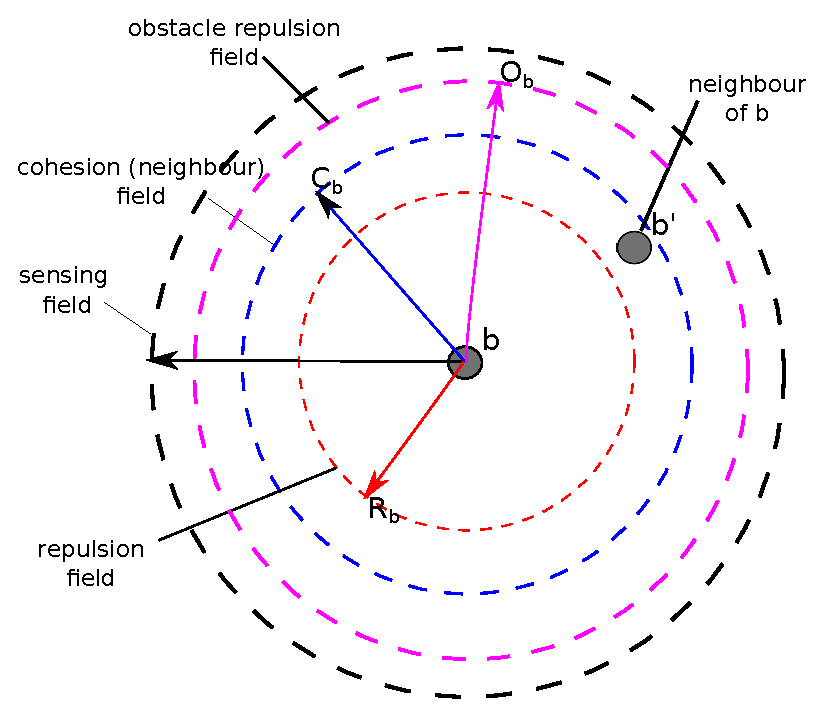
\includegraphics[width=6cm]{figures/FieldEffects}
\end{center}
\caption{Agent field effects\label{methods:FieldEffects}}
\end{figure}

Equation (\ref{eq:FlyToCentre1}) identifies the resultant cohesion effect of all the neighbours of $b$. $nbr(.)$ returns a set of all the agents in the swarm that are a neighbour of $b$. A neighbour is any agent that fails within the cohesion field.

\begin{equation}\label{eq:FlyToCentre1}
v_{c}(b) = \frac{\mathlarger{\sum_{b' \in nbr(b)}}{bb'}}{|nbr(b)|}
\end{equation}‎

Equation (\ref{eq:Repulsion1}) identifies the resultant repulsion effect of all the neighbours of $b$ where $rep(.)$ returns a set of all agents that are within the repulsion field.

\begin{equation}
\label{eq:Repulsion1}
v_{r}(b) =‎ -
\frac{1}{|R(b)|}
\left(
\mathlarger{\mathlarger{\sum_{b' \in rep(b)}}}
{\left( 1-\frac{|bb'|}{R_b} \right)}
{bb'}
\right)
\end{equation}‎

Using the cohesion and repulsion vectors generated by the relationship of $b$ to its neighbour a resultant vector can be calculated. This vector creates an agent characteristic that can be used as a metric. Summing the vectors creates a resultant vector with a magnitude that affects the agent. Summing the vectors also provides an indication of the direction an agent will move based on the relationship. This is the \textit{inter-agent vector}.

Equation (\ref{eq:InterAgentMovement1}) identifies the \textit{inter-agent vector} for agent $b$ with respect to its neighbours.

\begin{equation}\label{eq:InterAgentMovement1}
v(b) = v_{c}(b) + v_{r}(b)
\end{equation}‎

If the system is applying a weighted model then equation~\ref{eq:InterAgentMovement1} becomes:

\begin{equation}\label{eq:InterAgentMovement2}
v(b) = k_cv_{c}(b) + k_rv_{r}(b)
\end{equation}‎

To implement the boundary of an area a third component needs to be added to the model in the form of obstacles.

Obstacles, like agents, can be represented as a point in the system. As an agent moves an obstacles may enter its \textit{obstacle repulsion field} causing the agent move away.

In this thesis agents are modelled with a fixed obstacle repulsion distance $O_b$ where a repulsion vector is applied. The repulsion is then a vector of magnitude $O_b$. If more than one obstacle is within the field effect agent the total repulsion vector is the sum of the repulsion vectors due to each obstacle~(Figure~\ref{methods:Obstacle1}). The result is normalised and scaled such that the magnitude is the same as the field distance~$O_b$.

\begin{figure}
\begin{center}
\includegraphics[width=6cm]{figures/Obstacle1}
\end{center}
\caption{Obstacle repulsion \label{methods:Obstacle1}}
\end{figure}

%% $O$ is a set of $N$ obstacles.
%% 
%% \begin{center} \label{eq:Obstacle1}
%% \begin{equation}‎
%% O \buildrel \Delta \over =‎ \{o_1\ldots o_N\}
%% \end{equation}‎
%% \end{center}

%% $o' \in O:|bo'| < O_b$ the set of obstacles that are within range of agent $b$, where $O$ is the set of obstacles. 

%% \begin{center} \label{eq:Obstacle4}
%% \begin{equation}‎
%% R(b) \buildrel \Delta \over =‎ \{o' \in O:|bo'| < O_b\}
%% \end{equation}‎
%% \end{center}

Figure~\ref{eq:Obstacle2} shows the resultant repulsion vector $v_o(b)$ for an agent. $\{o\ \in O:|bo| <= O_b\}$ is the set of obstacles that are within range of agent $b$. $O$ is the set of obstacles. The obstacles are identified using the distance between an agent and an obstacle $|bo|$ and comparing the result to the fixed obstacle repulsion range~$O_b$. The result is calculated by scaling the normalised sum of the normalised vectors $(ob)\string^$ by $O_b$.

\begin{center} \label{eq:Obstacle2}
\begin{equation}‎
v_o(b) =‎ O_b\Bigg(\mathlarger{\mathlarger{\mathlarger{\sum}}}_{o \in O:|ob| <= O_b}(ob)\string^\Bigg)\string^
\end{equation}‎
\end{center}

%% \begin{center} \label{eq:Obstacle3}
%% \begin{equation}‎
%% v_o(b) =‎ |l_o(b)|O_b
%% \end{equation}‎
%% \end{center}as shown in equation~\ref{eq:InterAgentMovement3}.

The resultant swarm model is shown in~equation~\ref{eq:InterAgentMovement3}: 

\begin{equation}\label{eq:InterAgentMovement3}
v(b) = k_cv_{c}(b) + k_rv_{r}(b) + k_ov_{o}(b)
\end{equation}‎

\section{Area flooding}\label{chapter:flooding}
The concept of using a swarm to provide coverage over unknown areas is a current area of research. Alvissalim et al. (2012) discuss the application of commercially available drones to provide a communication infrastructure across an unknown disaster areas~\cite{AZHMJJM:12}. Scheutz and Bauer (2006) use both cohesion and repulsion as a mechanism to create coverage of an area that requires protection in an adversarial environment~\cite{SB:06}. In their paper they do not use cohesion to ensure the swarm remains a cohesive unit, rather they have all the agents using a \textit{destination vector} to cause agents to converge on a target and the repulsion vector prevents collisions. The cohesive effect is not required due to all agents having a common goal with no requirement for the agents to remain in close proximity during the terrain traversal. Ramaithitima et al. in 2015 and 2016, working as part of Vijay Kumar's research group at the University of Pennsylvania, use the idea of filling an area through a deployment strategy that requires the swarm to identify the placement of agents in a given space. The agents are then `shuffled' into an identified position. The technique applied in 2015~\cite{RWBK:15} is based upon coverage path planning and involves adding agents when required and does not require a global positioning reference. In their 2016 paper~\cite{RWBK:16} they use Voronoi graphs to achieve the same effect. Yang et al. (2015)~\cite{YDH:15} also use Voronoi graphs to achieve their swarm coverage goal. The use of Voronoi graphs requires inter-agent communications. Schroeder and M. Kumar (2016) use the bio-inspired swarming technique of creating chemical trails (pheromones) combined with a foraging approach which they refer to as a `food foraging' technique~\cite{SK:16}.

The techniques used in this paper are similar to Schroeder and M. Kumar in that the agents do not require a global positioning system and differ from Alvissalim et al., Scheutz and Bauer, and Ramaithitima et al. in that the space filling is achieved with a fixed sized swarm. 

The expansion fill is implemented using two techniques. The main principle behind both techniques is to increase the repulsion field effect of the agents over time to increase the area coverage of the agents. The expansion fill can use both the cohesion and repulsion field effects in a similar manner to a static swarm in free space. This technique ensures all the agents remain in close proximity and as far as possible the agents form a single entity. Alternatively the expansion fill can be implemented using only a repulsion field effect. Cohesion can be eliminated in an enclosed space as the agents have a limited range of movement (bounded by a perimeter). When agents move to a repulsion boundary, either an area perimeter or an obstacle, they are repelled. As the space is finite the repulsion `pushes' the agents back into the swarm countering the expansion that is induced by the \textit{interaction vectors}. If the repulsion field effect creates a swarm that reaches all the boundaries the repulsion imposes a compression effect as the \textit{interaction-vector} `pushes' the agents into the boundaries. 

\section{Field effect modification with cohesion and repulsion}
The concept behind the field effect expansion is to increase both the repulsion and cohesion fields over a period of time. This increase in the field effects makes the agents increase the distance between each other expanding the swarm as a whole. The expansion increases until, due to boundary compression, the swarm is unable to expand further. In an extreme case the expansion will result in a set of field effects that create a mesh based swarm structure rather than the desired hexagonal structure that the field effects should create. Identifying either the change in modality or the inability to expand, which can be identified by the \textit{inter-agent vector magnitude} increase or a reduction in the inter-agent distance stability indicates area saturation has occured.

To test this hypothesis a swarm is modelled in the simulator. The model consists of an obstacle-based enclosed space and a swarm consisting of 60 agents. The experiments parameters for the simulation are shown in~Table~\ref{tab:FillParameters}

\begin{table}
\begin{center}
\begin{tabular}{| p{1.5cm} | p{1.5cm} | p{4.0cm} |}
\hline
\bf Parameter & \bf Value  & \bf Description \\ \hline
$k_c$         & 5          & weight adjuster for cohesion bias\\ \hline
$k_r$         & 60         & weight adjuster for repulsion bias\\ \hline
Sample rate   & 100ms      & proximity sensor rate\\ \hline
Speed         & 20 units/s & agent speed\\ \hline
\end{tabular}\caption{Swarm parameters} \label{tab:FillParameters}
\end{center}
\end{table}

The field effects are incremented in turn, neighbour range followed by repulsion range. After each repulsion field change the swarm is allowed to redistribute itself and stabilise. Table~\ref{tab:BaselineConcaveReduction} shows the field settings that are used for the simulation. The field effect are selected so as to ensure the swarm parameters have the potential to create a hexagonal swarm. 

\begin{table}
\begin{center}
\begin{tabular}{| p{1.5cm} | p{0.3cm} | p{0.3cm} | p{0.3cm} | p{0.3cm} | p{0.3cm} | p{0.3cm} | p{0.3cm} | p{0.5cm} |}
\hline
\bf Weight \bf component & \bf 1 & \bf 2 & \bf 3 & \bf 4 & \bf 5 & \bf 6 & \bf 7 & \\ \hline
Repulsion Boundary & 50 & -  & 60 & -  & 70 & -  & 80 & units\\  \hline
Neighbour Distance & 60 & 70 & -  & 80 & -  & 90 & -  & units\\  \hline
\end{tabular}\caption{field effect expansion sequence} \label{tab:FillSequence}
\end{center}
\end{table}

Figures~\ref{emerge:Expand1}, \ref{emerge:Expand2}, \ref{emerge:Expand3}, \ref{emerge:Expand4}, \ref{emerge:Expand5} and \ref{emerge:Expand6} show the stages that the swarm progresses through during the simulation. Figure~\ref{emerge:Expand1} shows the initial deployment of the 60 agents within the enclosed environment. Figure~\ref{emerge:Expand6} shows the stage at which the experiment terminates due to area saturation.

\begin{figure}
\begin{center}
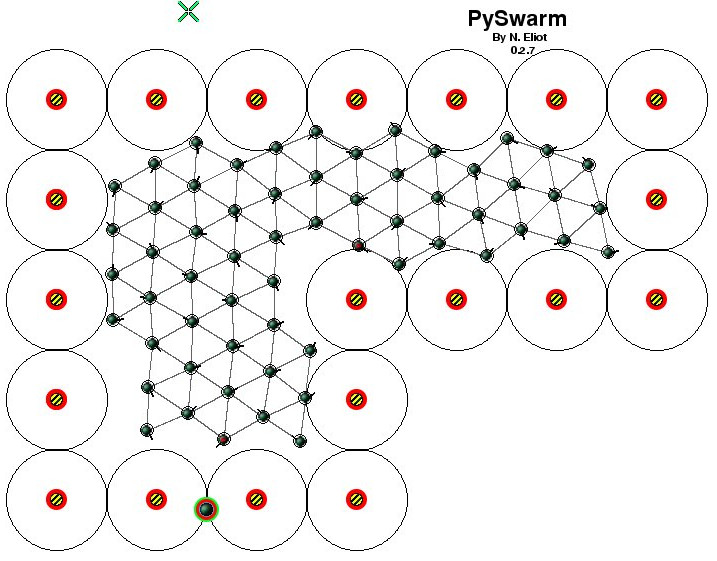
\includegraphics[width=5.5cm]{figures/EXPAND1}
\end{center}
\caption{Stage 1\label{emerge:Expand1}}
\end{figure}

\begin{figure}
\begin{center}
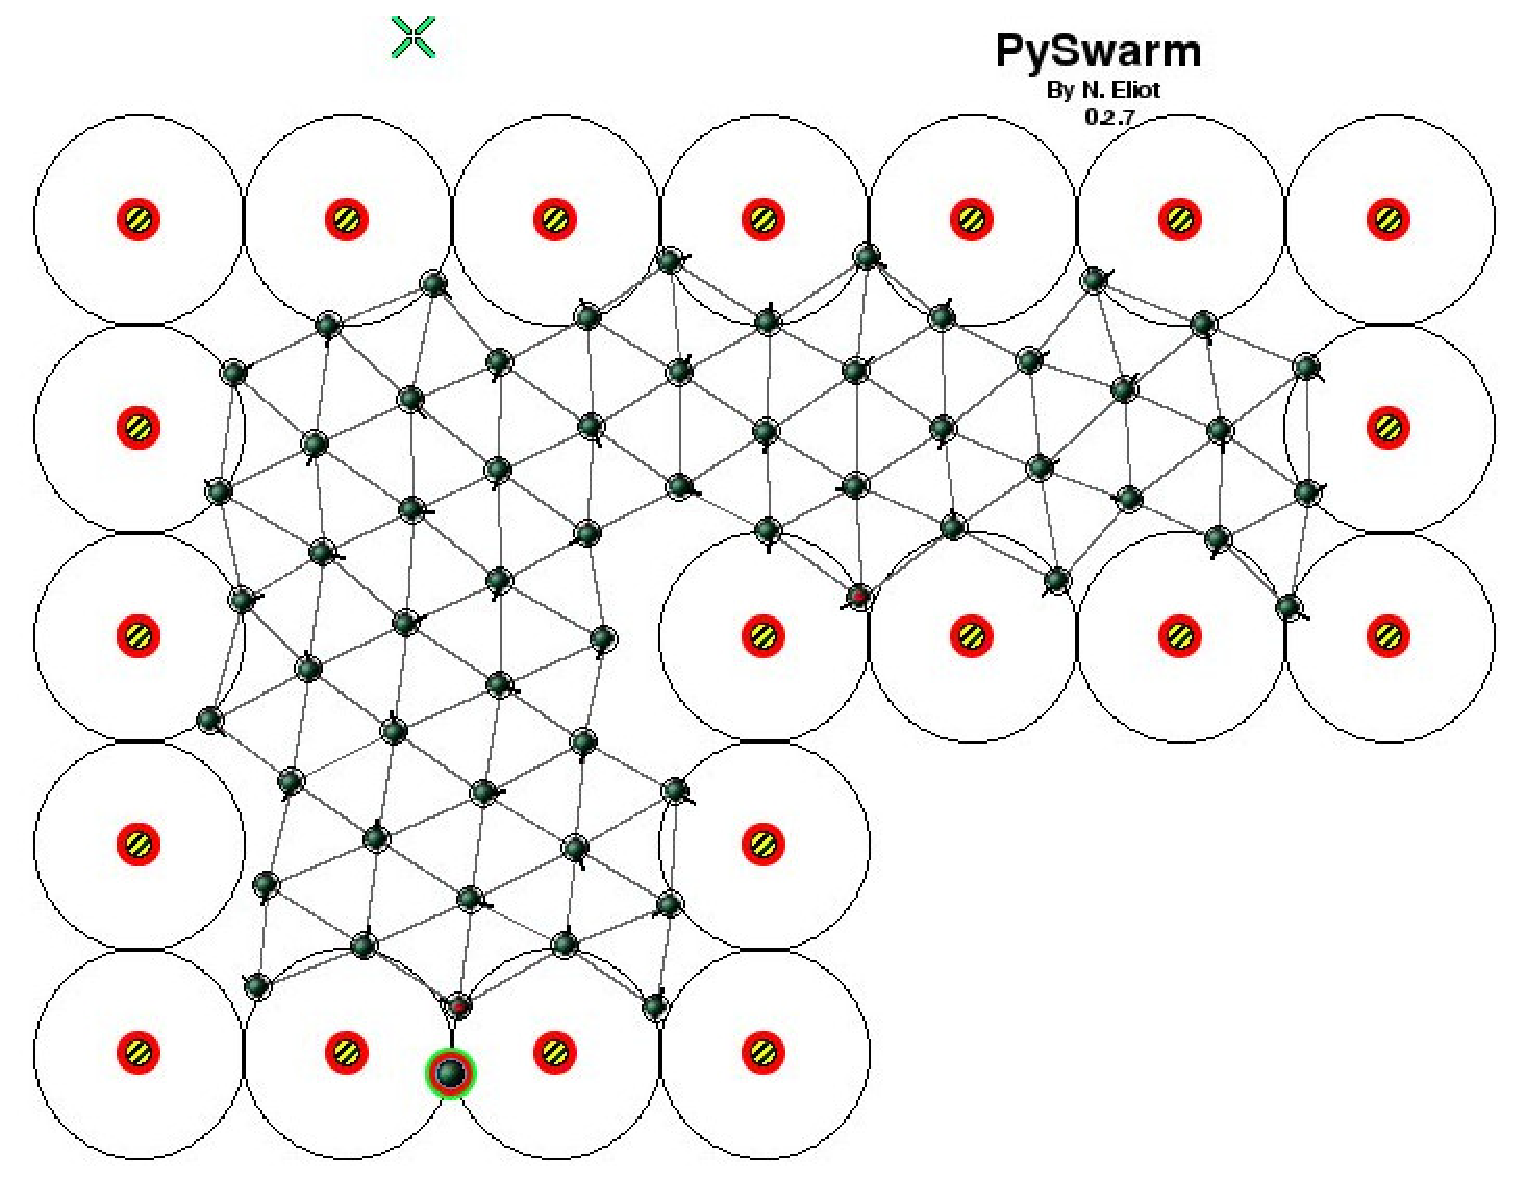
\includegraphics[width=5.5cm]{figures/EXPAND2}
\end{center}
\caption{Stage 2\label{emerge:Expand2}}
\end{figure}

\begin{figure}
\begin{center}
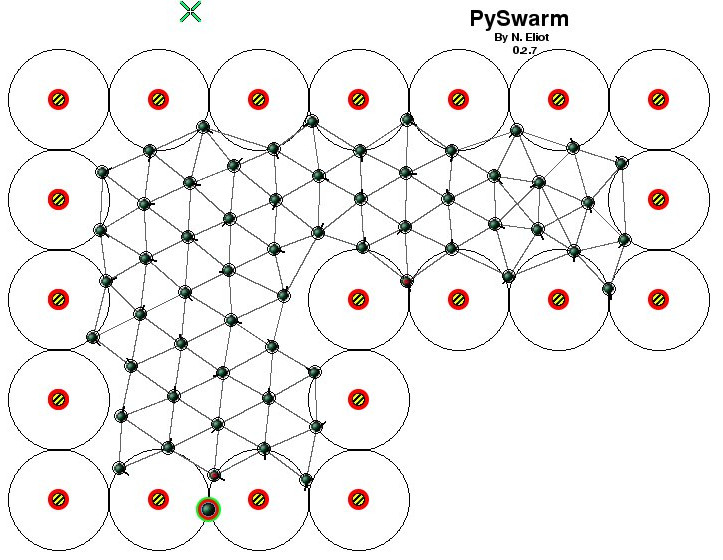
\includegraphics[width=5.5cm]{figures/EXPAND3}
\end{center}
\caption{Stage 3\label{emerge:Expand3}}
\end{figure}

\begin{figure}
\begin{center}
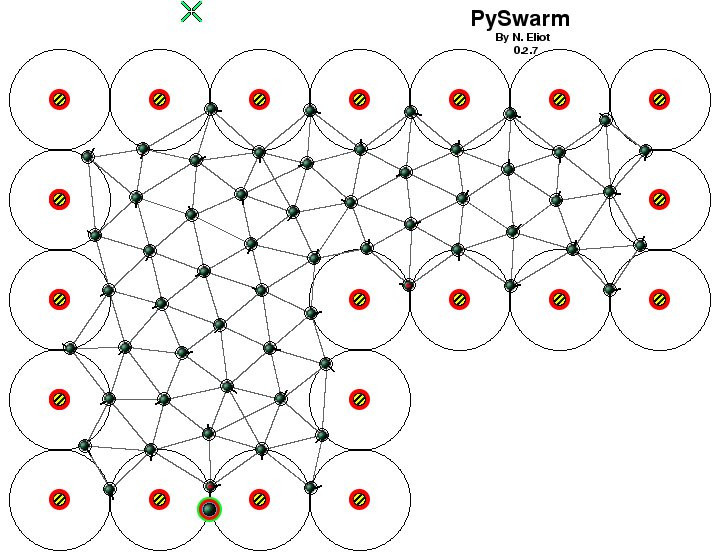
\includegraphics[width=5.5cm]{figures/EXPAND4}
\end{center}
\caption{Stage 4\label{emerge:Expand4}}
\end{figure}

\begin{figure}
\begin{center}
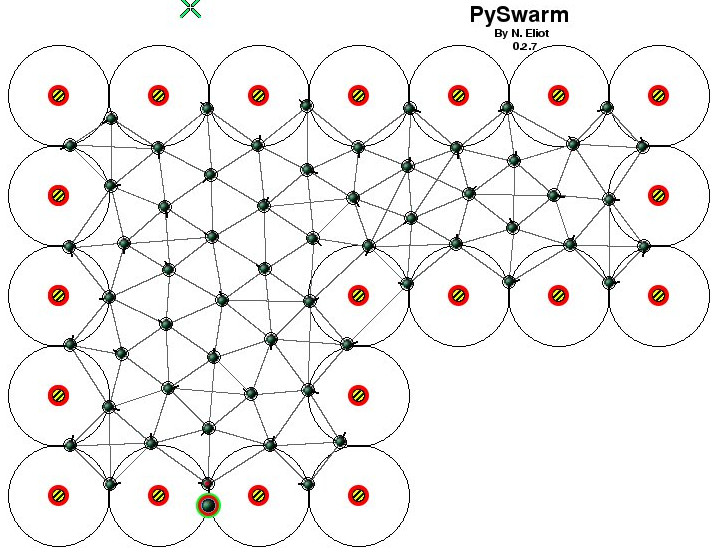
\includegraphics[width=5.5cm]{figures/EXPAND5}
\end{center}
\caption{Stage 5\label{emerge:Expand5}}
\end{figure}

\begin{figure}
\begin{center}
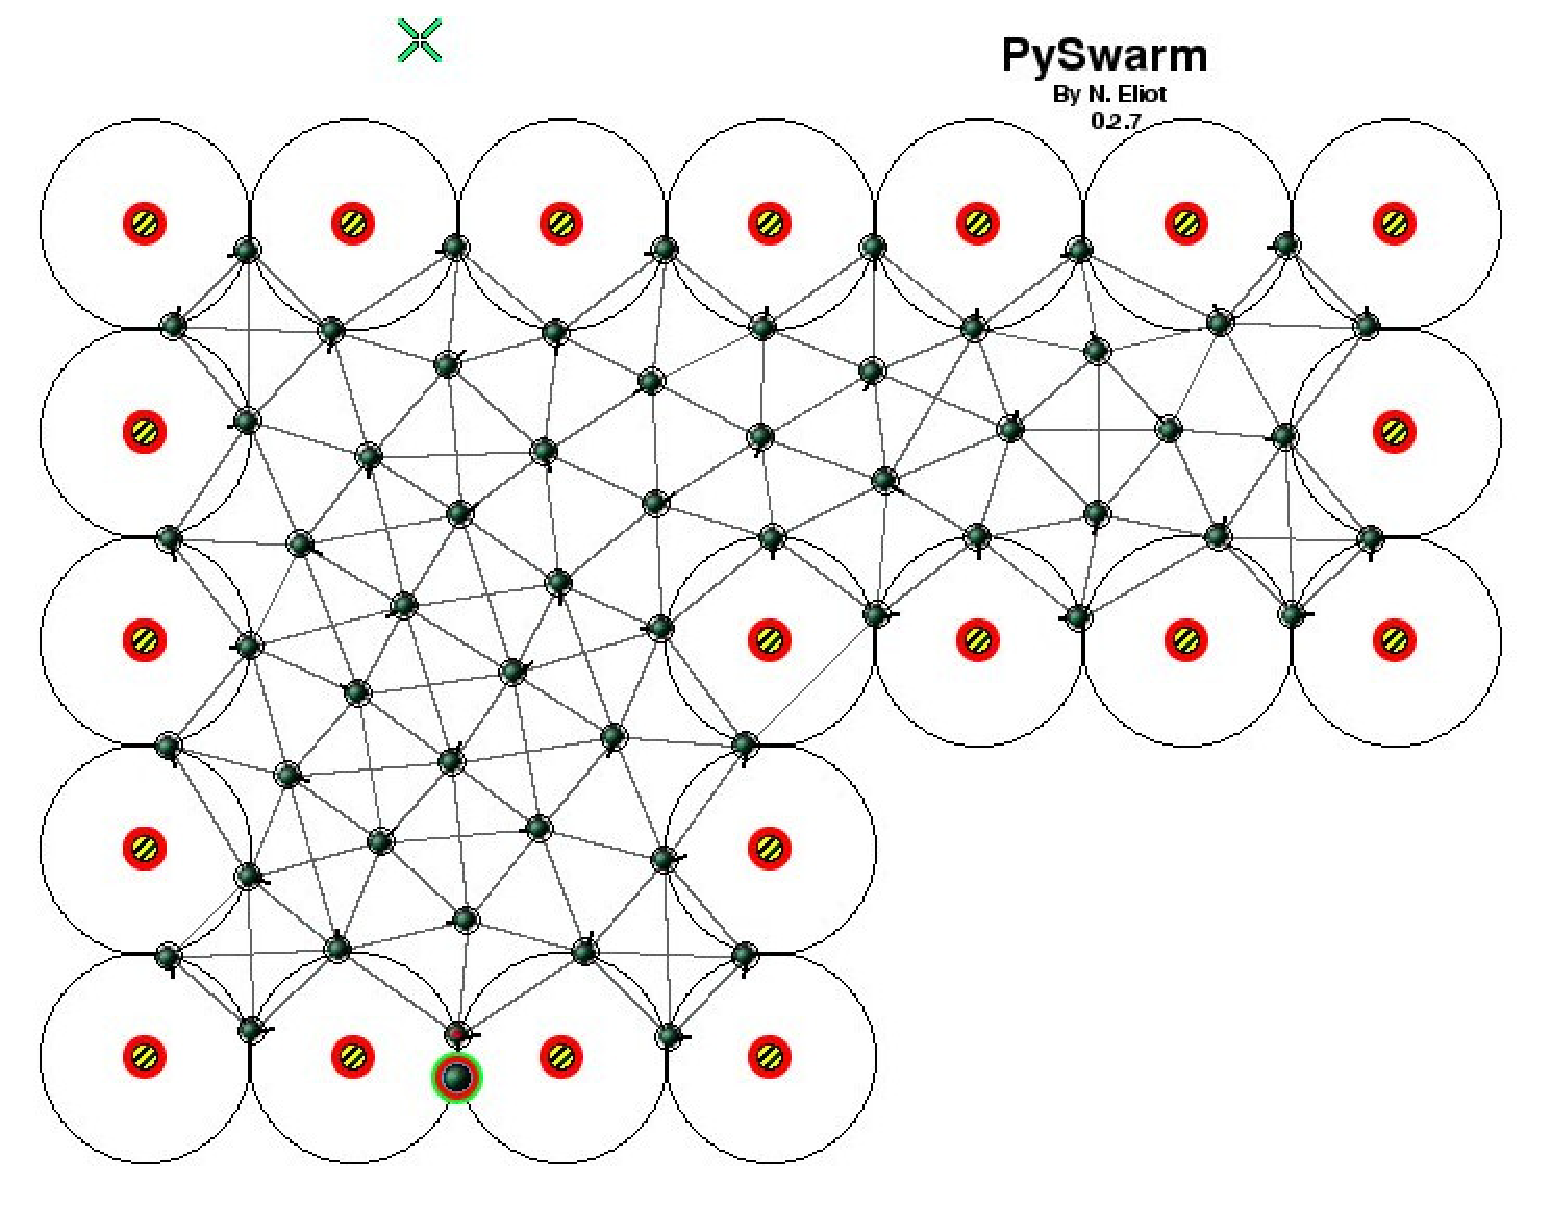
\includegraphics[width=5.5cm]{figures/EXPAND6}
\end{center}
\caption{Stage 6\label{emerge:Expand6}}
\end{figure}

%% \begin{figure}
%% \centering
%% \subfigure[Stage 1]{
%% 	 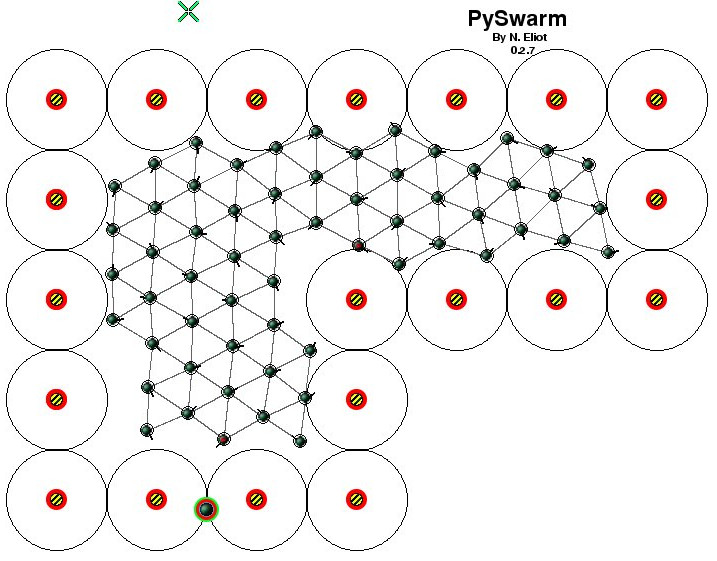
\includegraphics[width=5.5cm]{figures/EXPAND1}
%% 	 \label{emerge:Expand1}
%% }
%% \subfigure[Stage 2]{
%% 	 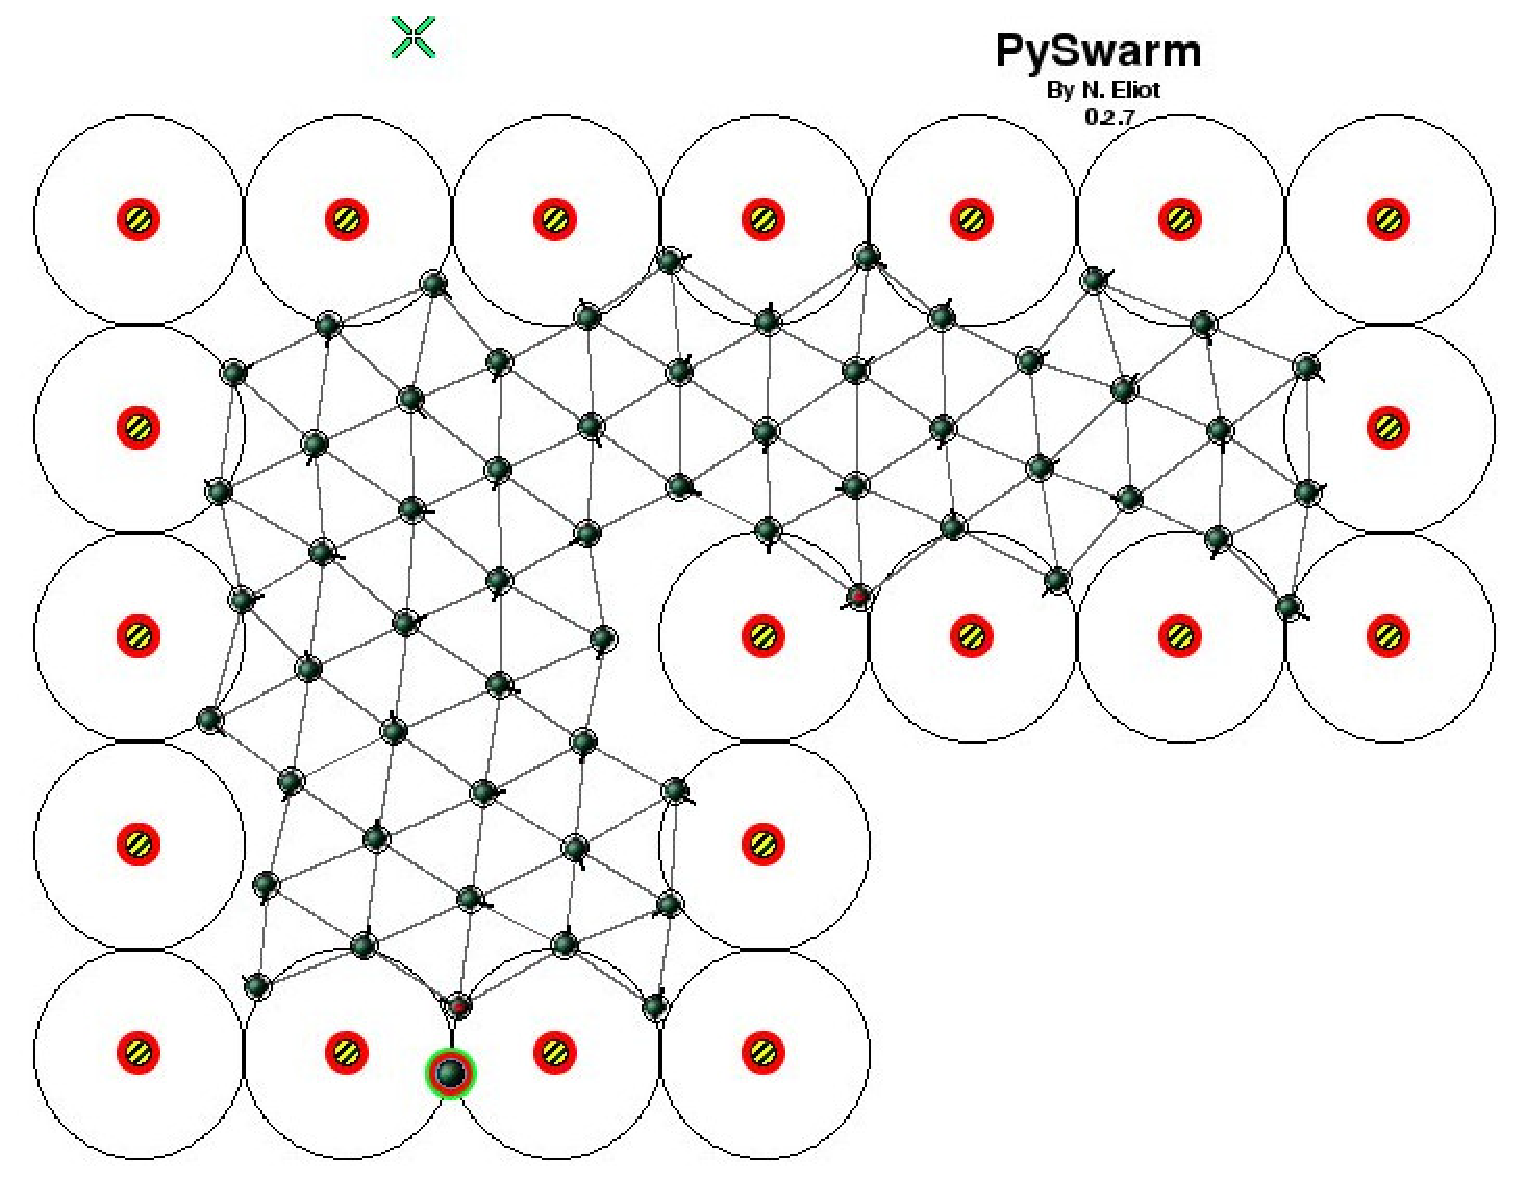
\includegraphics[width=5.5cm]{figures/EXPAND2}
%% 	 \label{emerge:Expand2}
%% }
%% \subfigure[Stage 3]{
%% 	 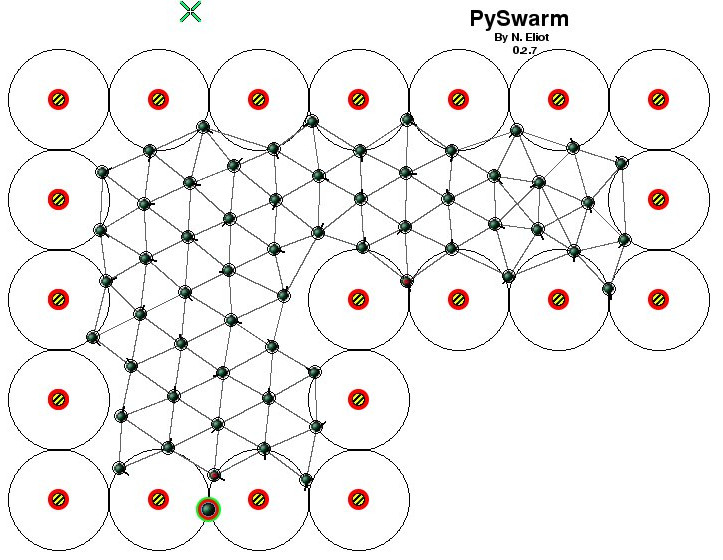
\includegraphics[width=5.5cm]{figures/EXPAND3}
%% 	 \label{emerge:Expand3}
%% }
%% \subfigure[Stage 4]{
%% 	 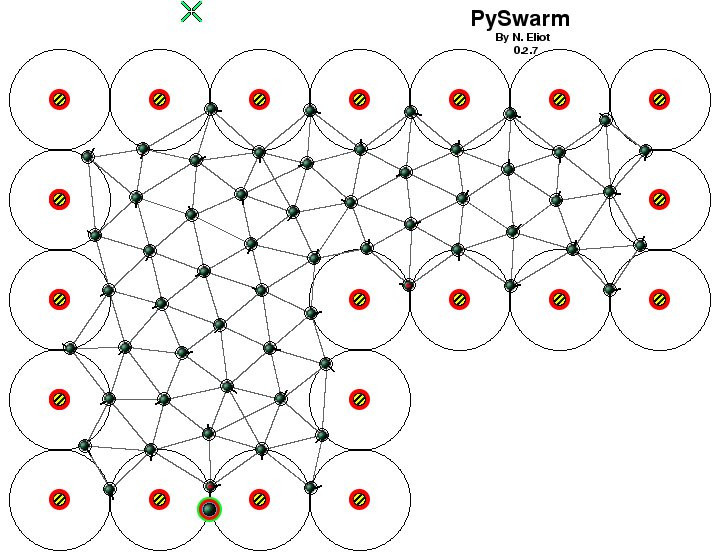
\includegraphics[width=5.5cm]{figures/EXPAND4}
%% 	 \label{emerge:Expand4}
%% }
%% \subfigure[Stage 5]{
%% 	 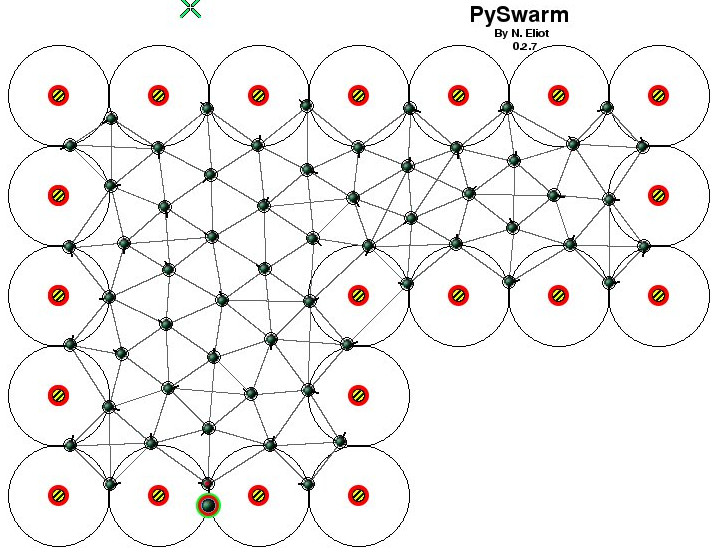
\includegraphics[width=5.5cm]{figures/EXPAND5}
%% 	 \label{emerge:Expand5}
%% }
%% \subfigure[Stage 6]{
%% 	 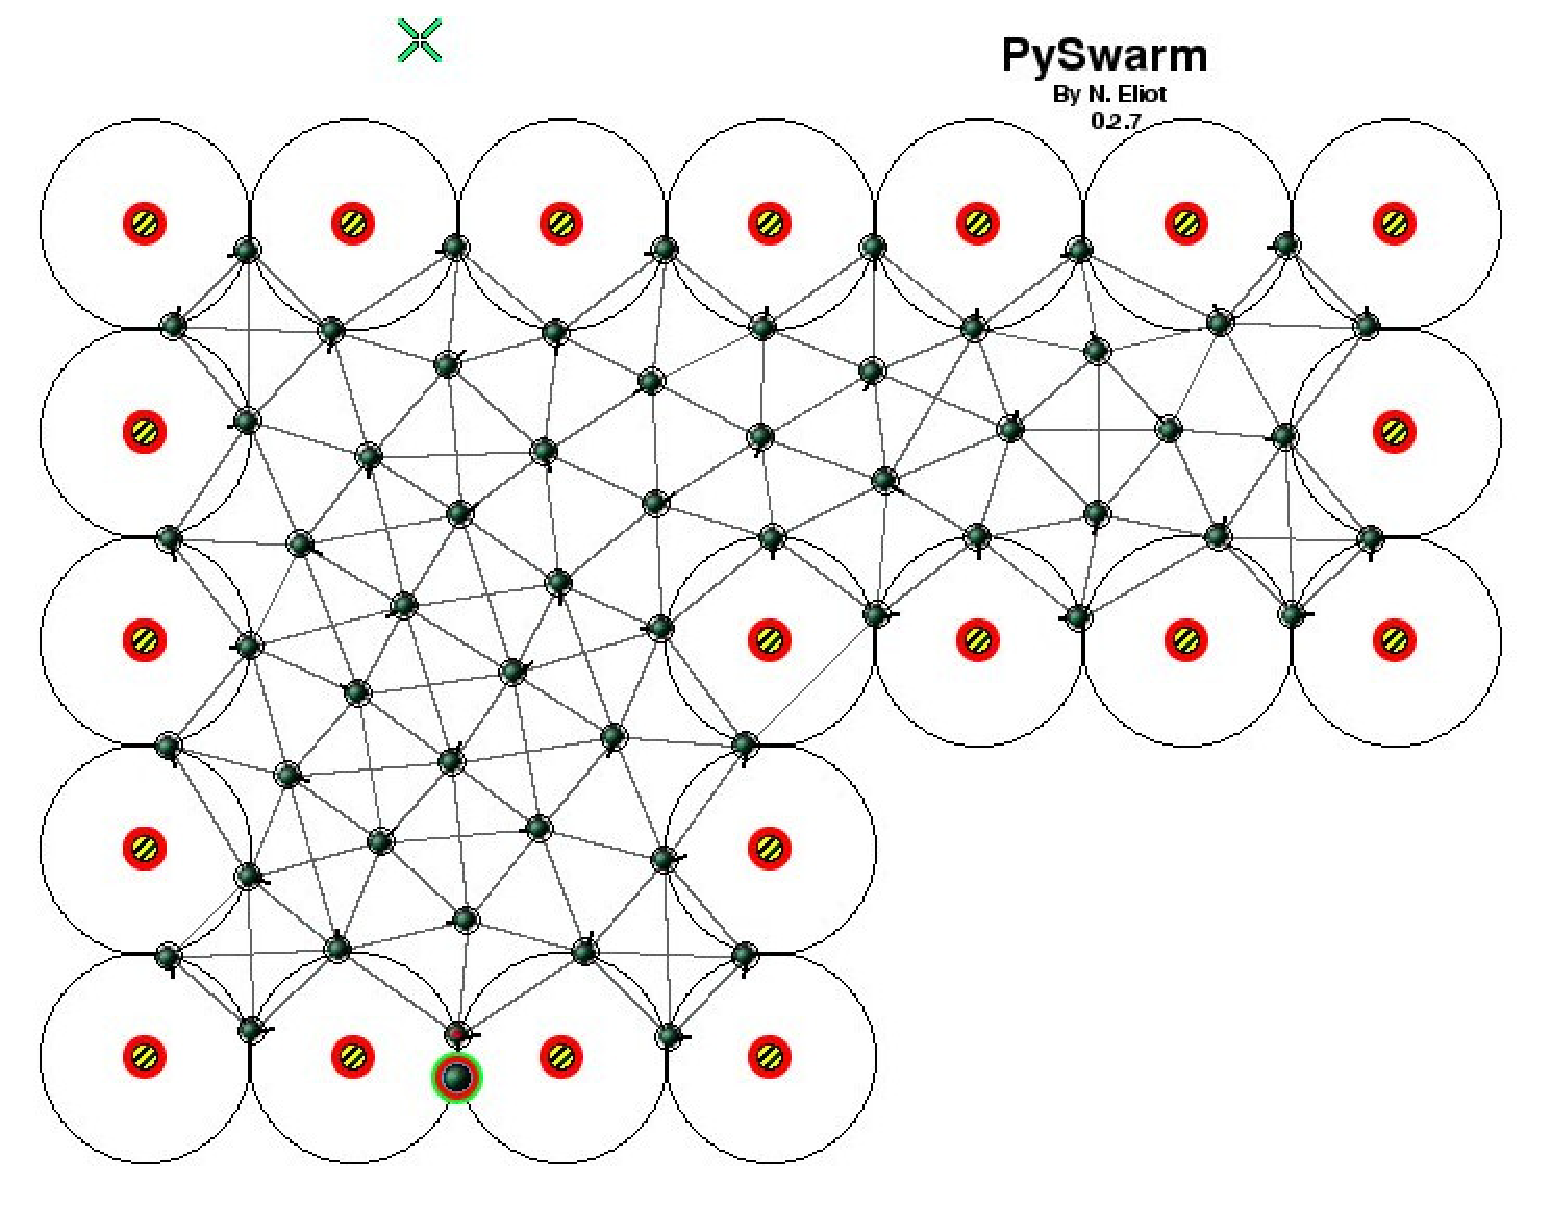
\includegraphics[width=5.5cm]{figures/EXPAND6}
%% 	 \label{emerge:Expand6}
%% }
%% \caption{Space filling via field effect expansion}
%% \label{methods:ExpansionFill}
%% \end{figure}

After the initial deployment the system is allowed to settle~Figure~(\ref{emerge:Expand2}) following the settling period the parameters are increased and the swarm settles again. Figure~\ref{emerge:Expand3}~shows how the change in parameters can cause the system to become unstable, the top right section of the swarm has became multi-modal yet there is still a section of the swarm that has not expanded to the boundary perimeter. As the swarm stabilises this compressed section of the swarm `pushes' through the swarm and the swarm increases in volume filling more of the space~(Figure~\ref{emerge:Expand4}). This process continues until changes in the parameters are unable to increase the distribution of the agents and the distances remain almost constant. Increasing the field effects further causes the swarm to become multi-modal as shown in~Figures~\ref{emerge:Expand5} and~\ref{emerge:Expand6}.

These effects can be identified through a combination of the \textit{inter-agent magnitude metric} and the distance metric.

\subsection{Magnitude analysis}
Figure~\ref{emerge:FIELDFILL-MAG} shows the resultant magnitude for the swarm for the entire simulation. Between 100 seconds and 105 seconds there is a significant change in the magnitude where the value becomes negative. This indicates there is a compression effect on the swarm and it is unable to expand the inter-agent distances.

\begin{figure}
\begin{center}
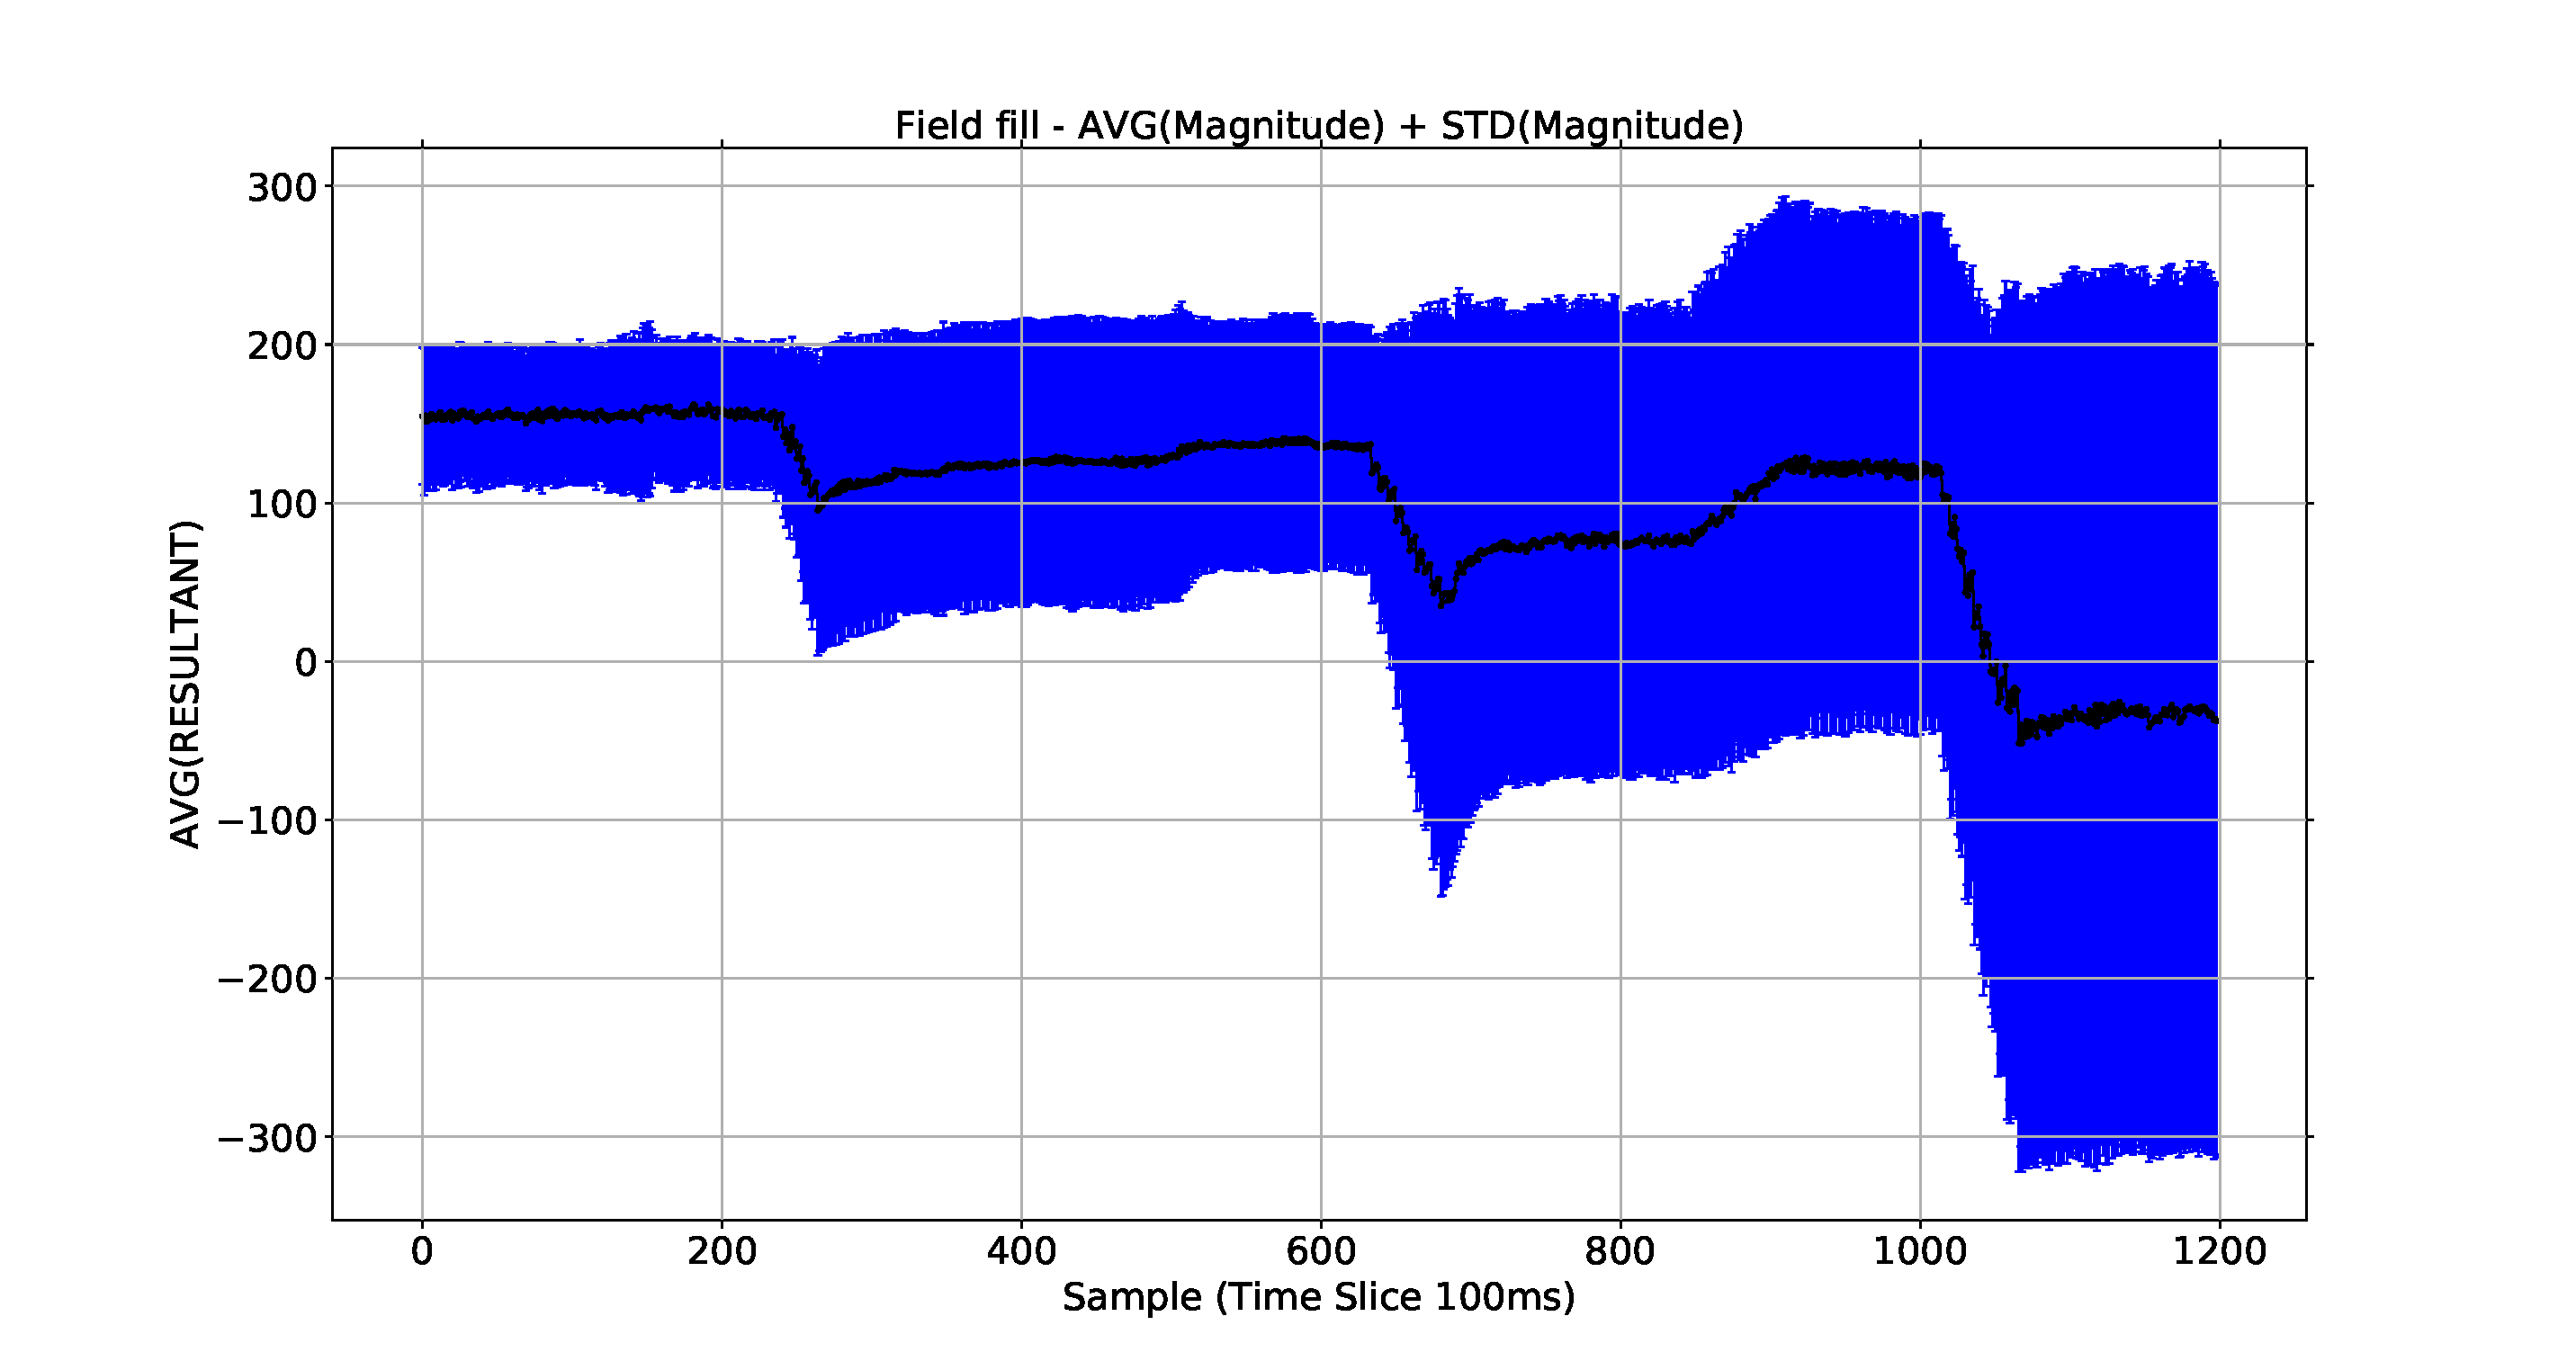
\includegraphics[width=8.5cm]{figures/FIELDFILL-MAG}
\end{center}
\caption{Magnitude metric 0-120 seconds\label{emerge:FIELDFILL-MAG}}
\end{figure}

Figure~\ref{emerge:FIELDFILL-MAG-1} shows the initial deployment status of the swarm and the first repulsion increase at 25 seconds. When the repulsion field is increased, the average \textit{inter-agent magnitude} falls and the variation increases. The agents redistribute themselves which takes until approximately 65 seconds and a new baseline is established for the field effects.

\begin{figure}
\begin{center}
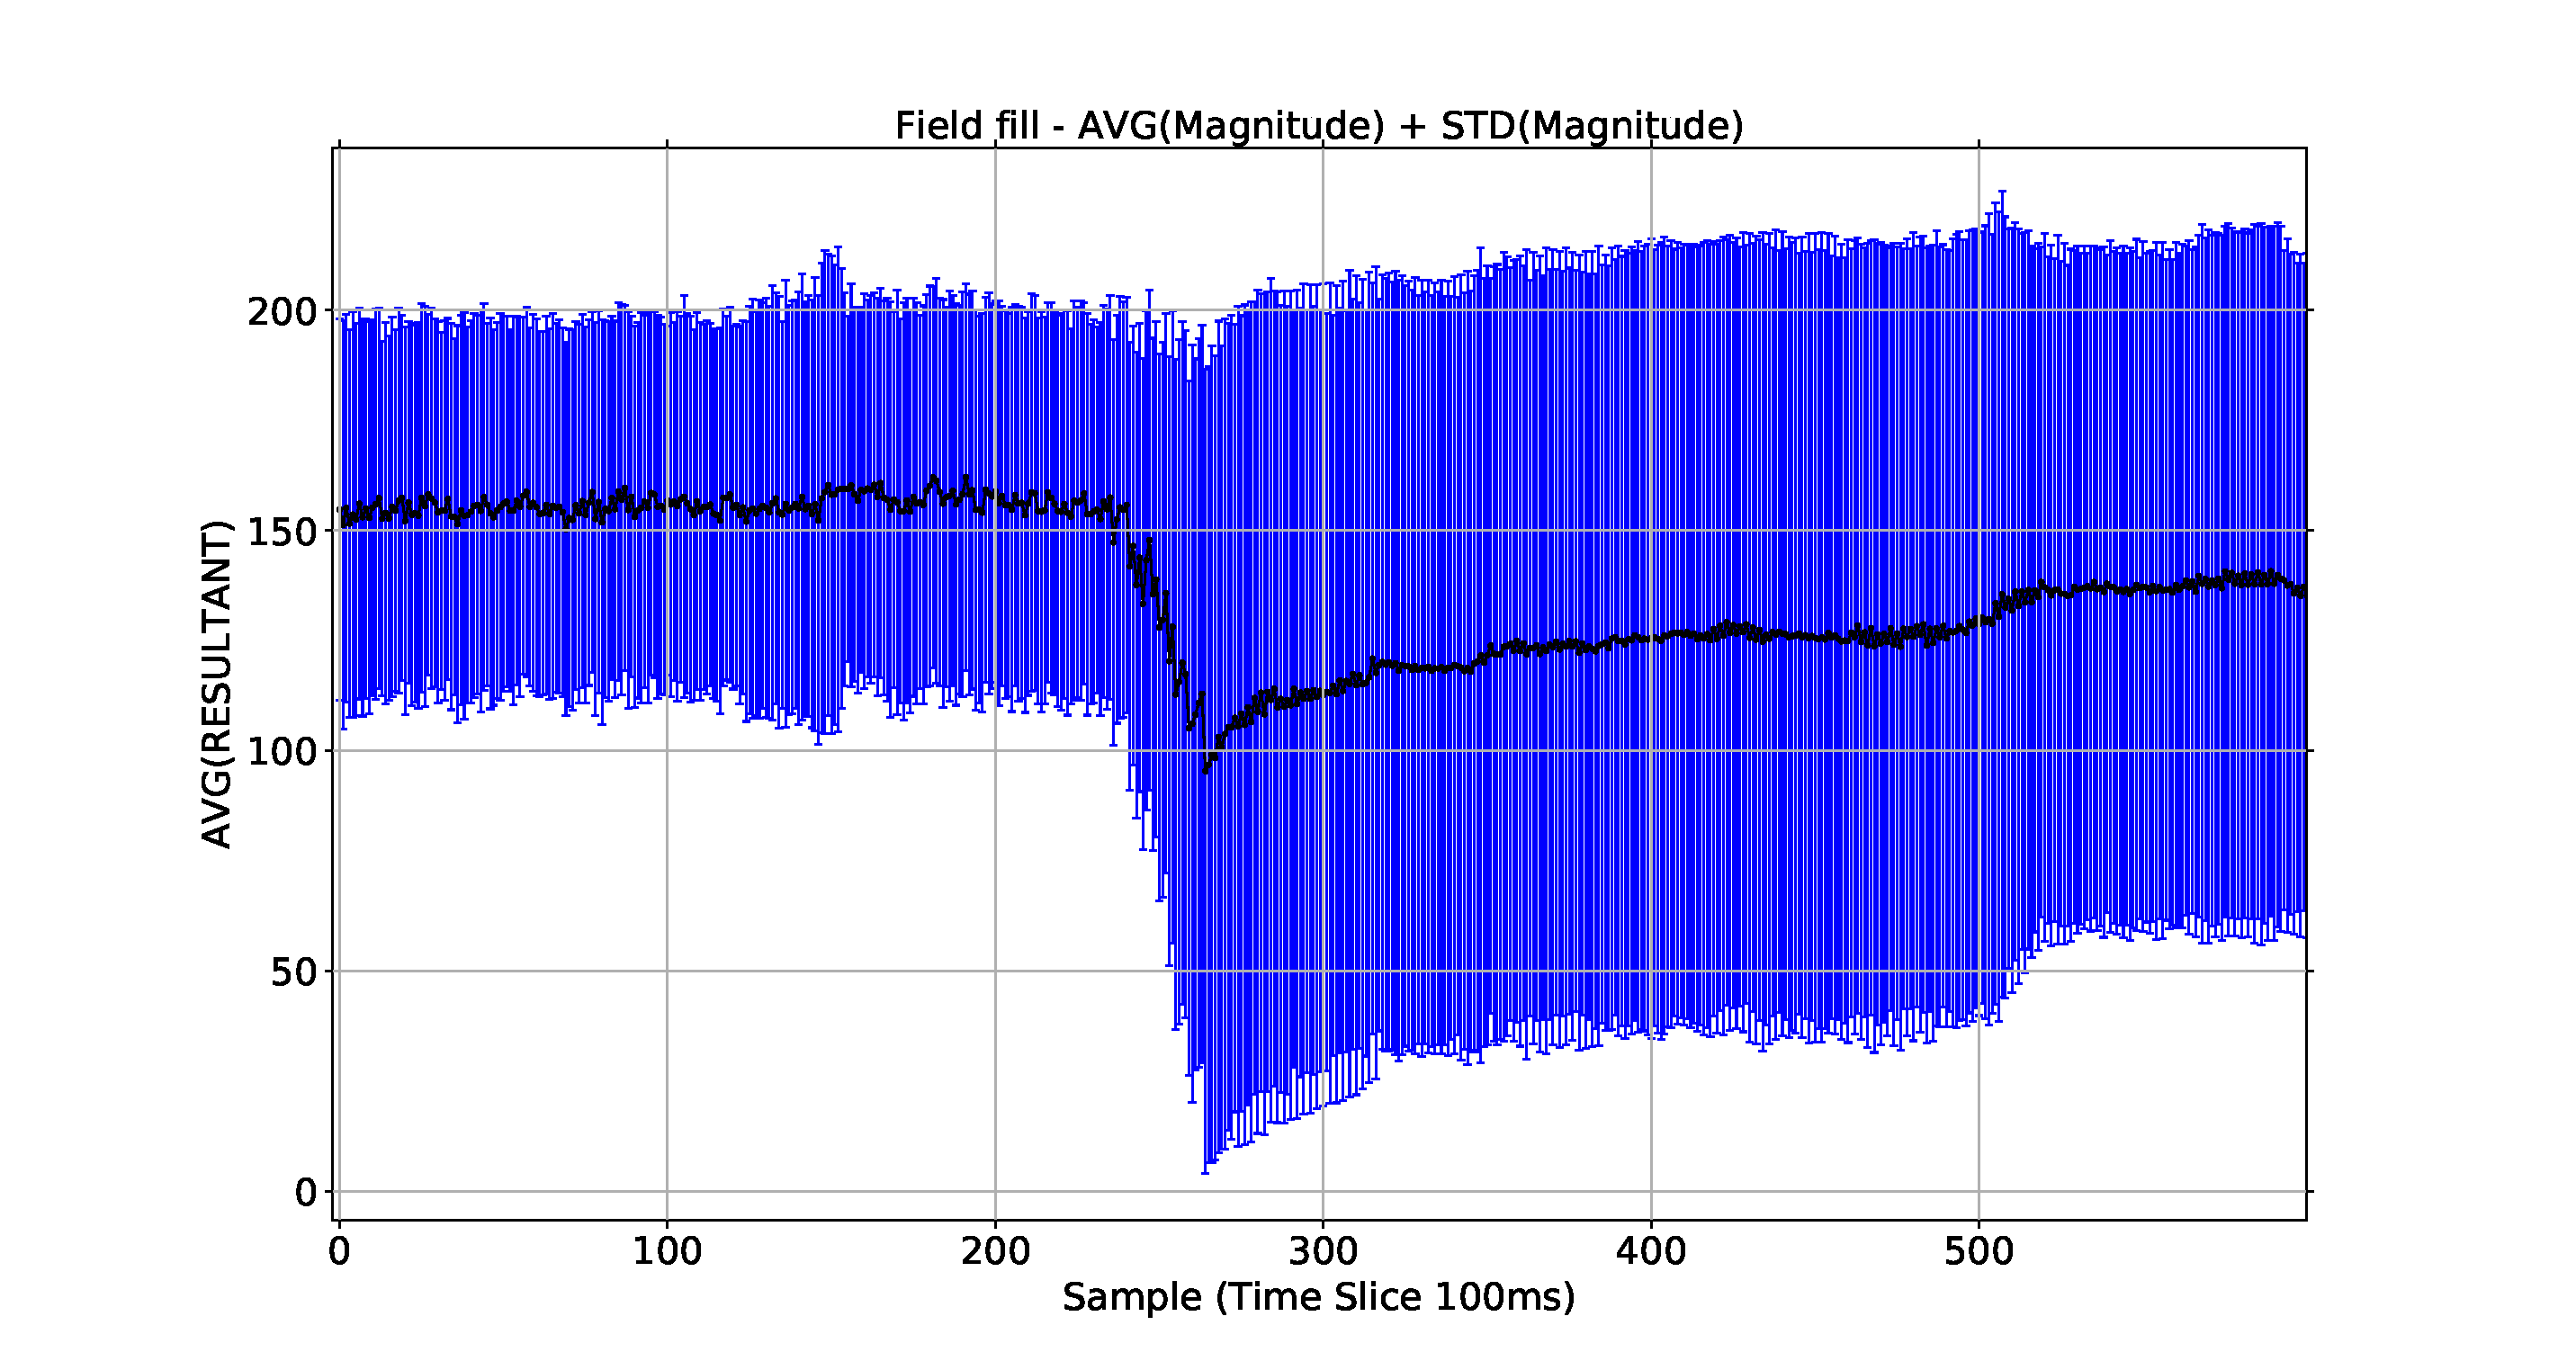
\includegraphics[width=8.5cm]{figures/FIELDFILL-MAG-1}
\end{center}
\caption{Magnitude metric 0-60 seconds\label{emerge:FIELDFILL-MAG-1}}
\end{figure}

The next increment at 65 seconds creates a similar reaction to the magnitude and variance and the swarm settles to another baseline, however, the new baseline has a variance which drops the rseultant magnitude to below zero. This indicates that some of the swarm is experiencing a compression effect which will result in the swarm body moving towards an uncompressed area. At 85 seconds the next repulsion increase is made and the reaction of the swarm metrics indicates something has changed in how the swarm is reacting. The average \textit{inter-agent magnitude} rises and the variance increases. This change is the effect of an increase in the modality of the swarm which indicates that the swarm is fully distributed within the environment as the neighbour field effect is detecting additional neighbour agents. The final increment at 108 seconds creates an even greater increase in the variance, this is caused by a further increase in the modal distribution of the agents and the swarm is being compressed by the boundary of the space.

\begin{figure}
\begin{center}
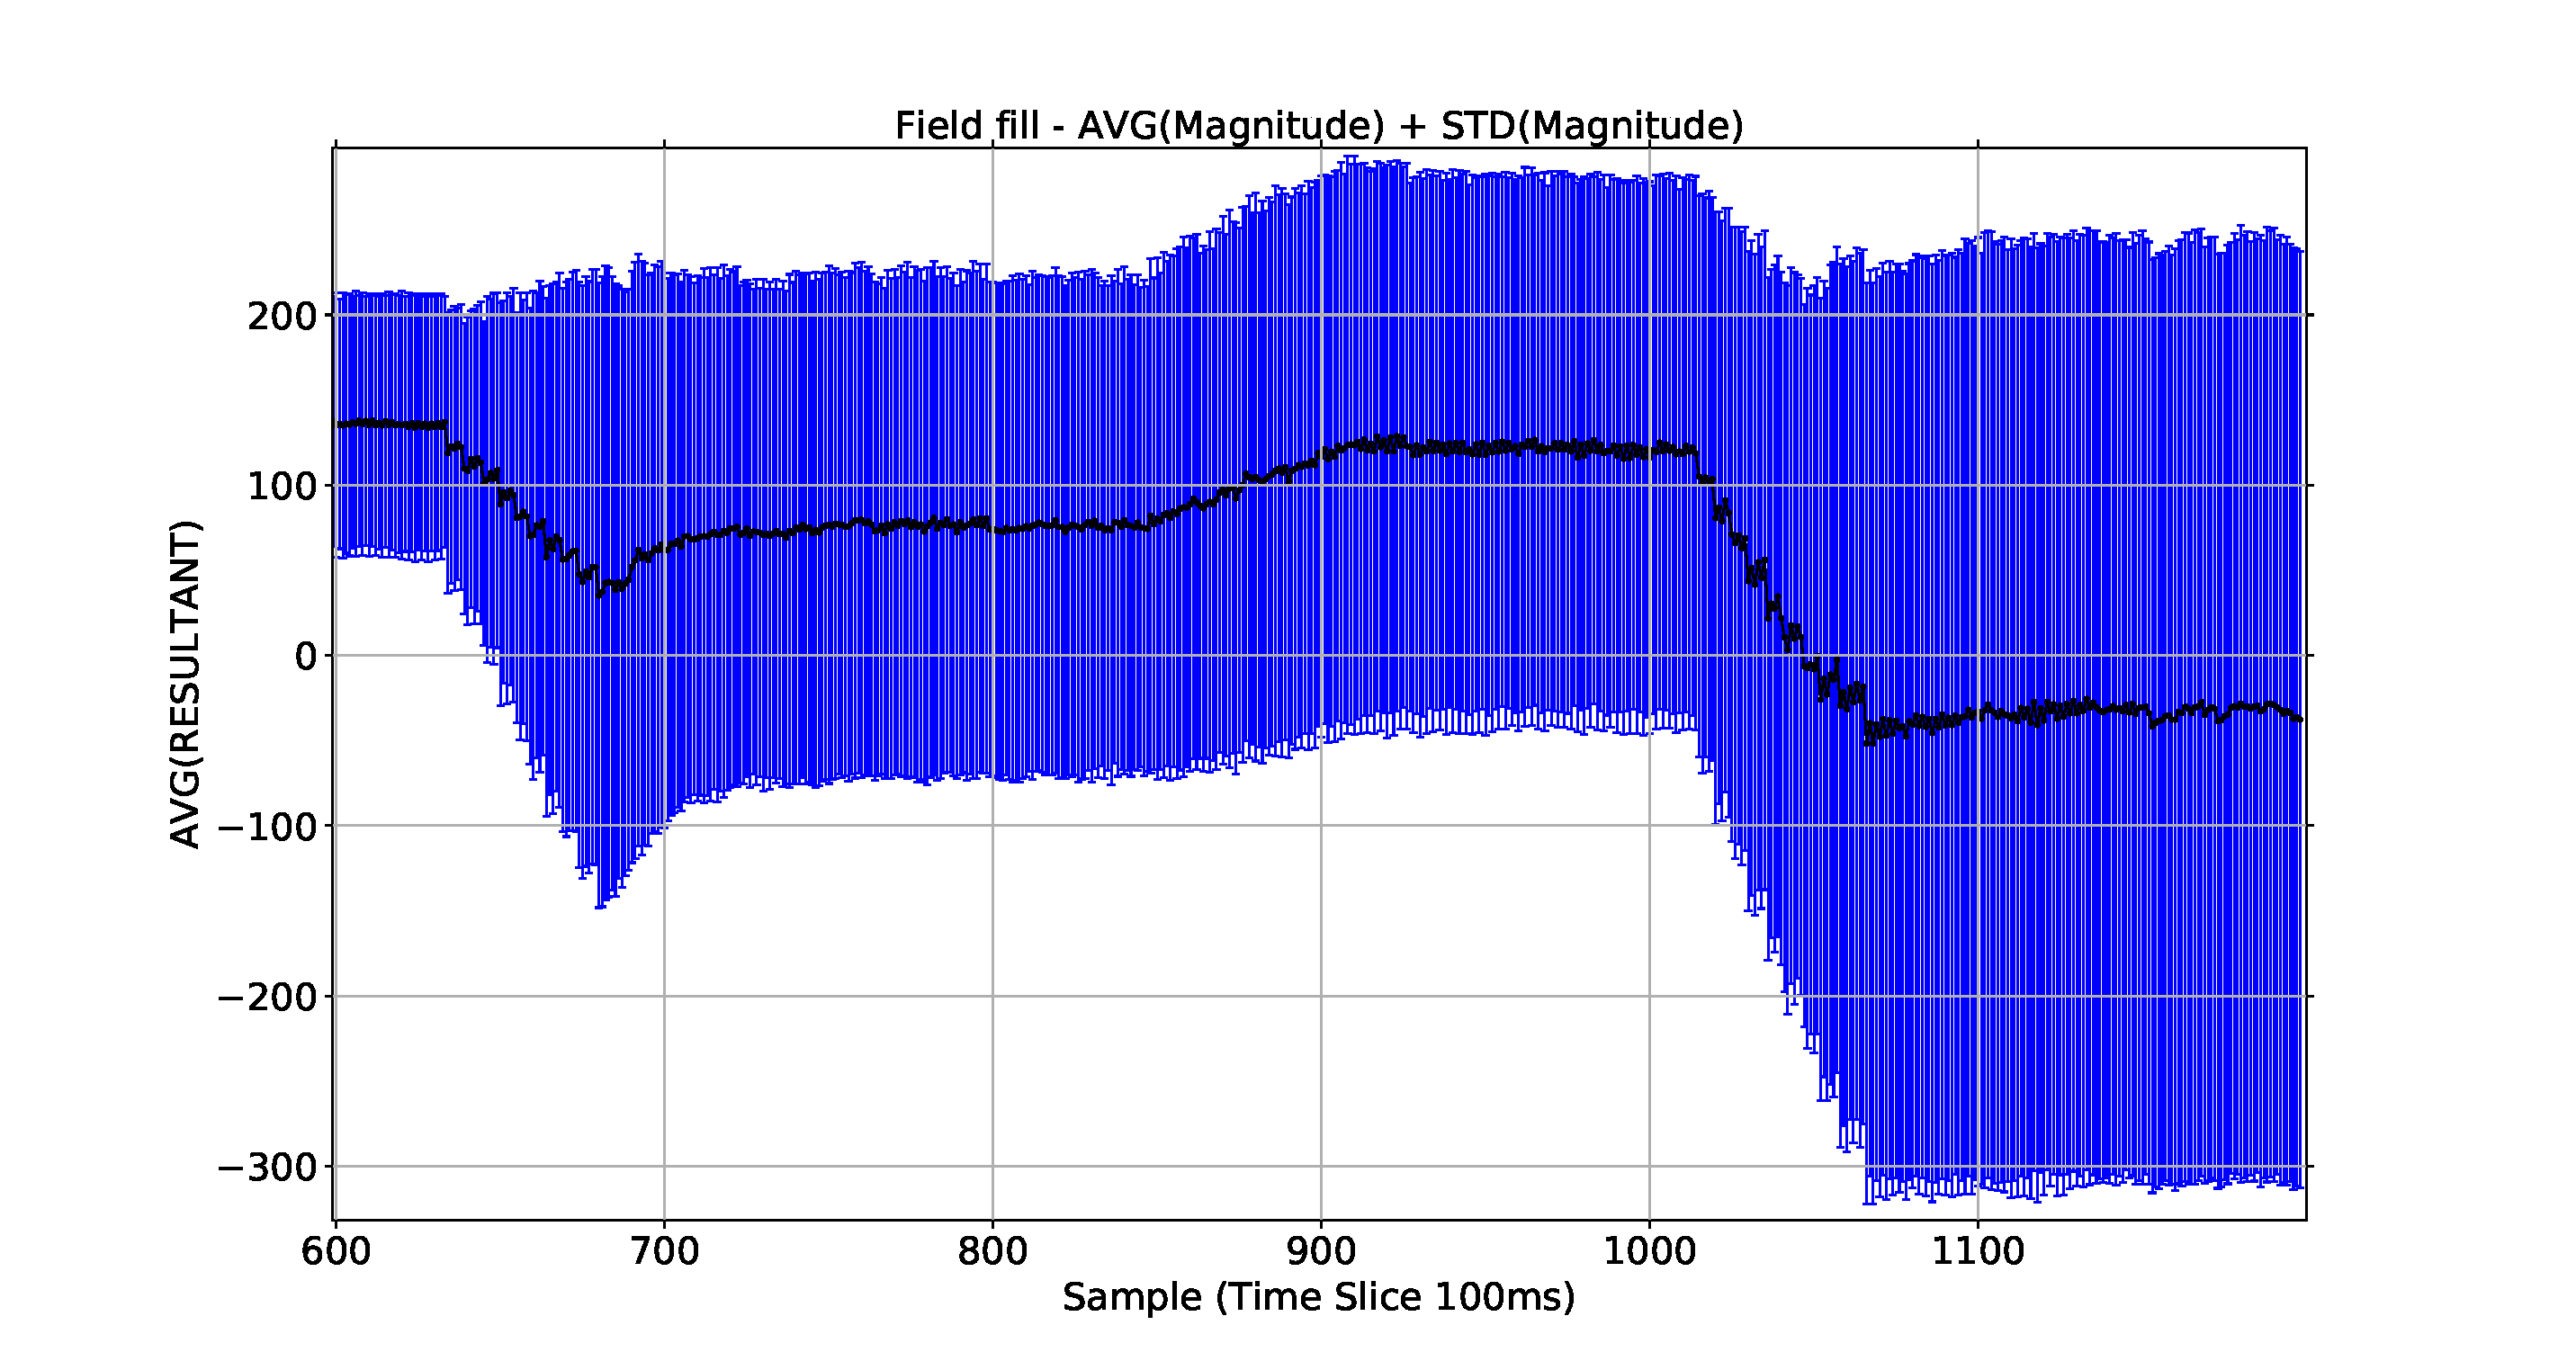
\includegraphics[width=8.5cm]{figures/FIELDFILL-MAG-2}
\end{center}
\caption{Magnitude metric 60-120 seconds\label{emerge:FIELDFILL-MAG-2}}
\end{figure}

\subsection{Distance analysis}
Figure~\ref{emerge:FIELDFILL-DIST}~shows the distance metric for the simulation. The initial deployment is shown at 0 seconds followed by incremental changes in the distances and variance of the distances as each increment is made in the field effects. The simulation terminates after 12 seconds.

\begin{figure}
\begin{center}
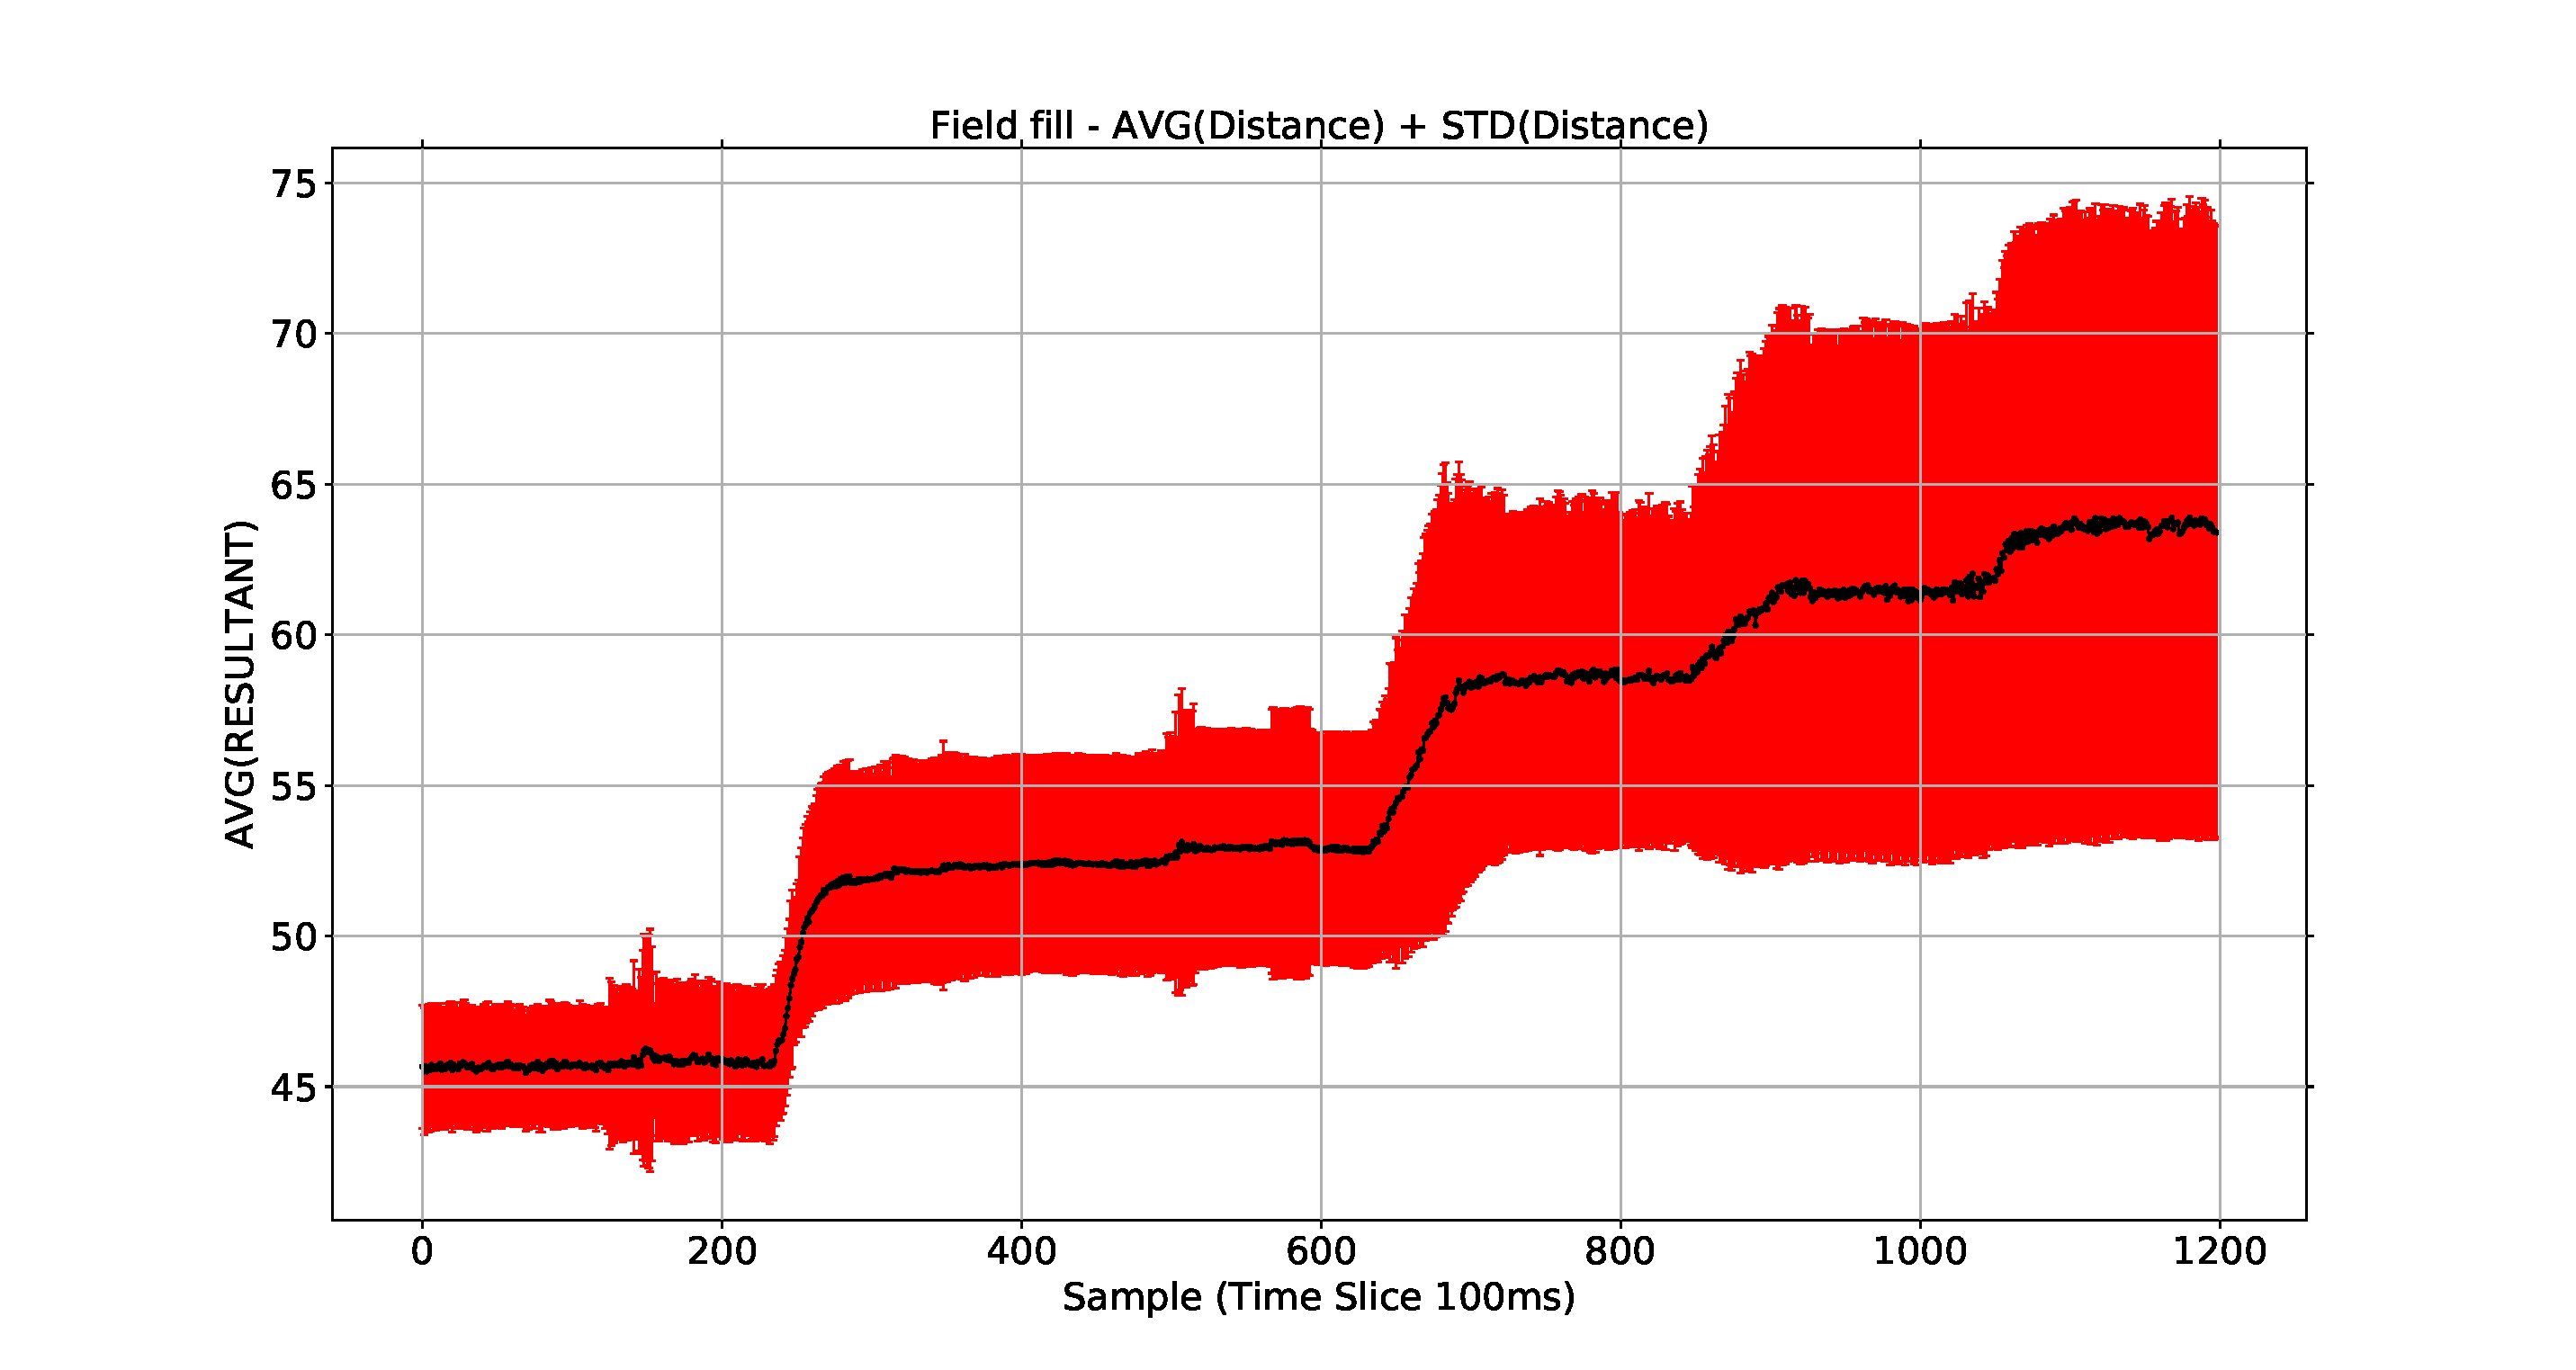
\includegraphics[width=8.5cm]{figures/FIELDFILL-DIST}
\end{center}
\caption{Distance metric 0-120 seconds\label{emerge:FIELDFILL-DIST}}
\end{figure}

Figure~\ref{emerge:FIELDFILL-DIST-1} shows the initial expansion increasing the field distance causing the agents to `spread' throughout the space. each increment having a settling period as the swarm expands.

\begin{figure}
\begin{center}
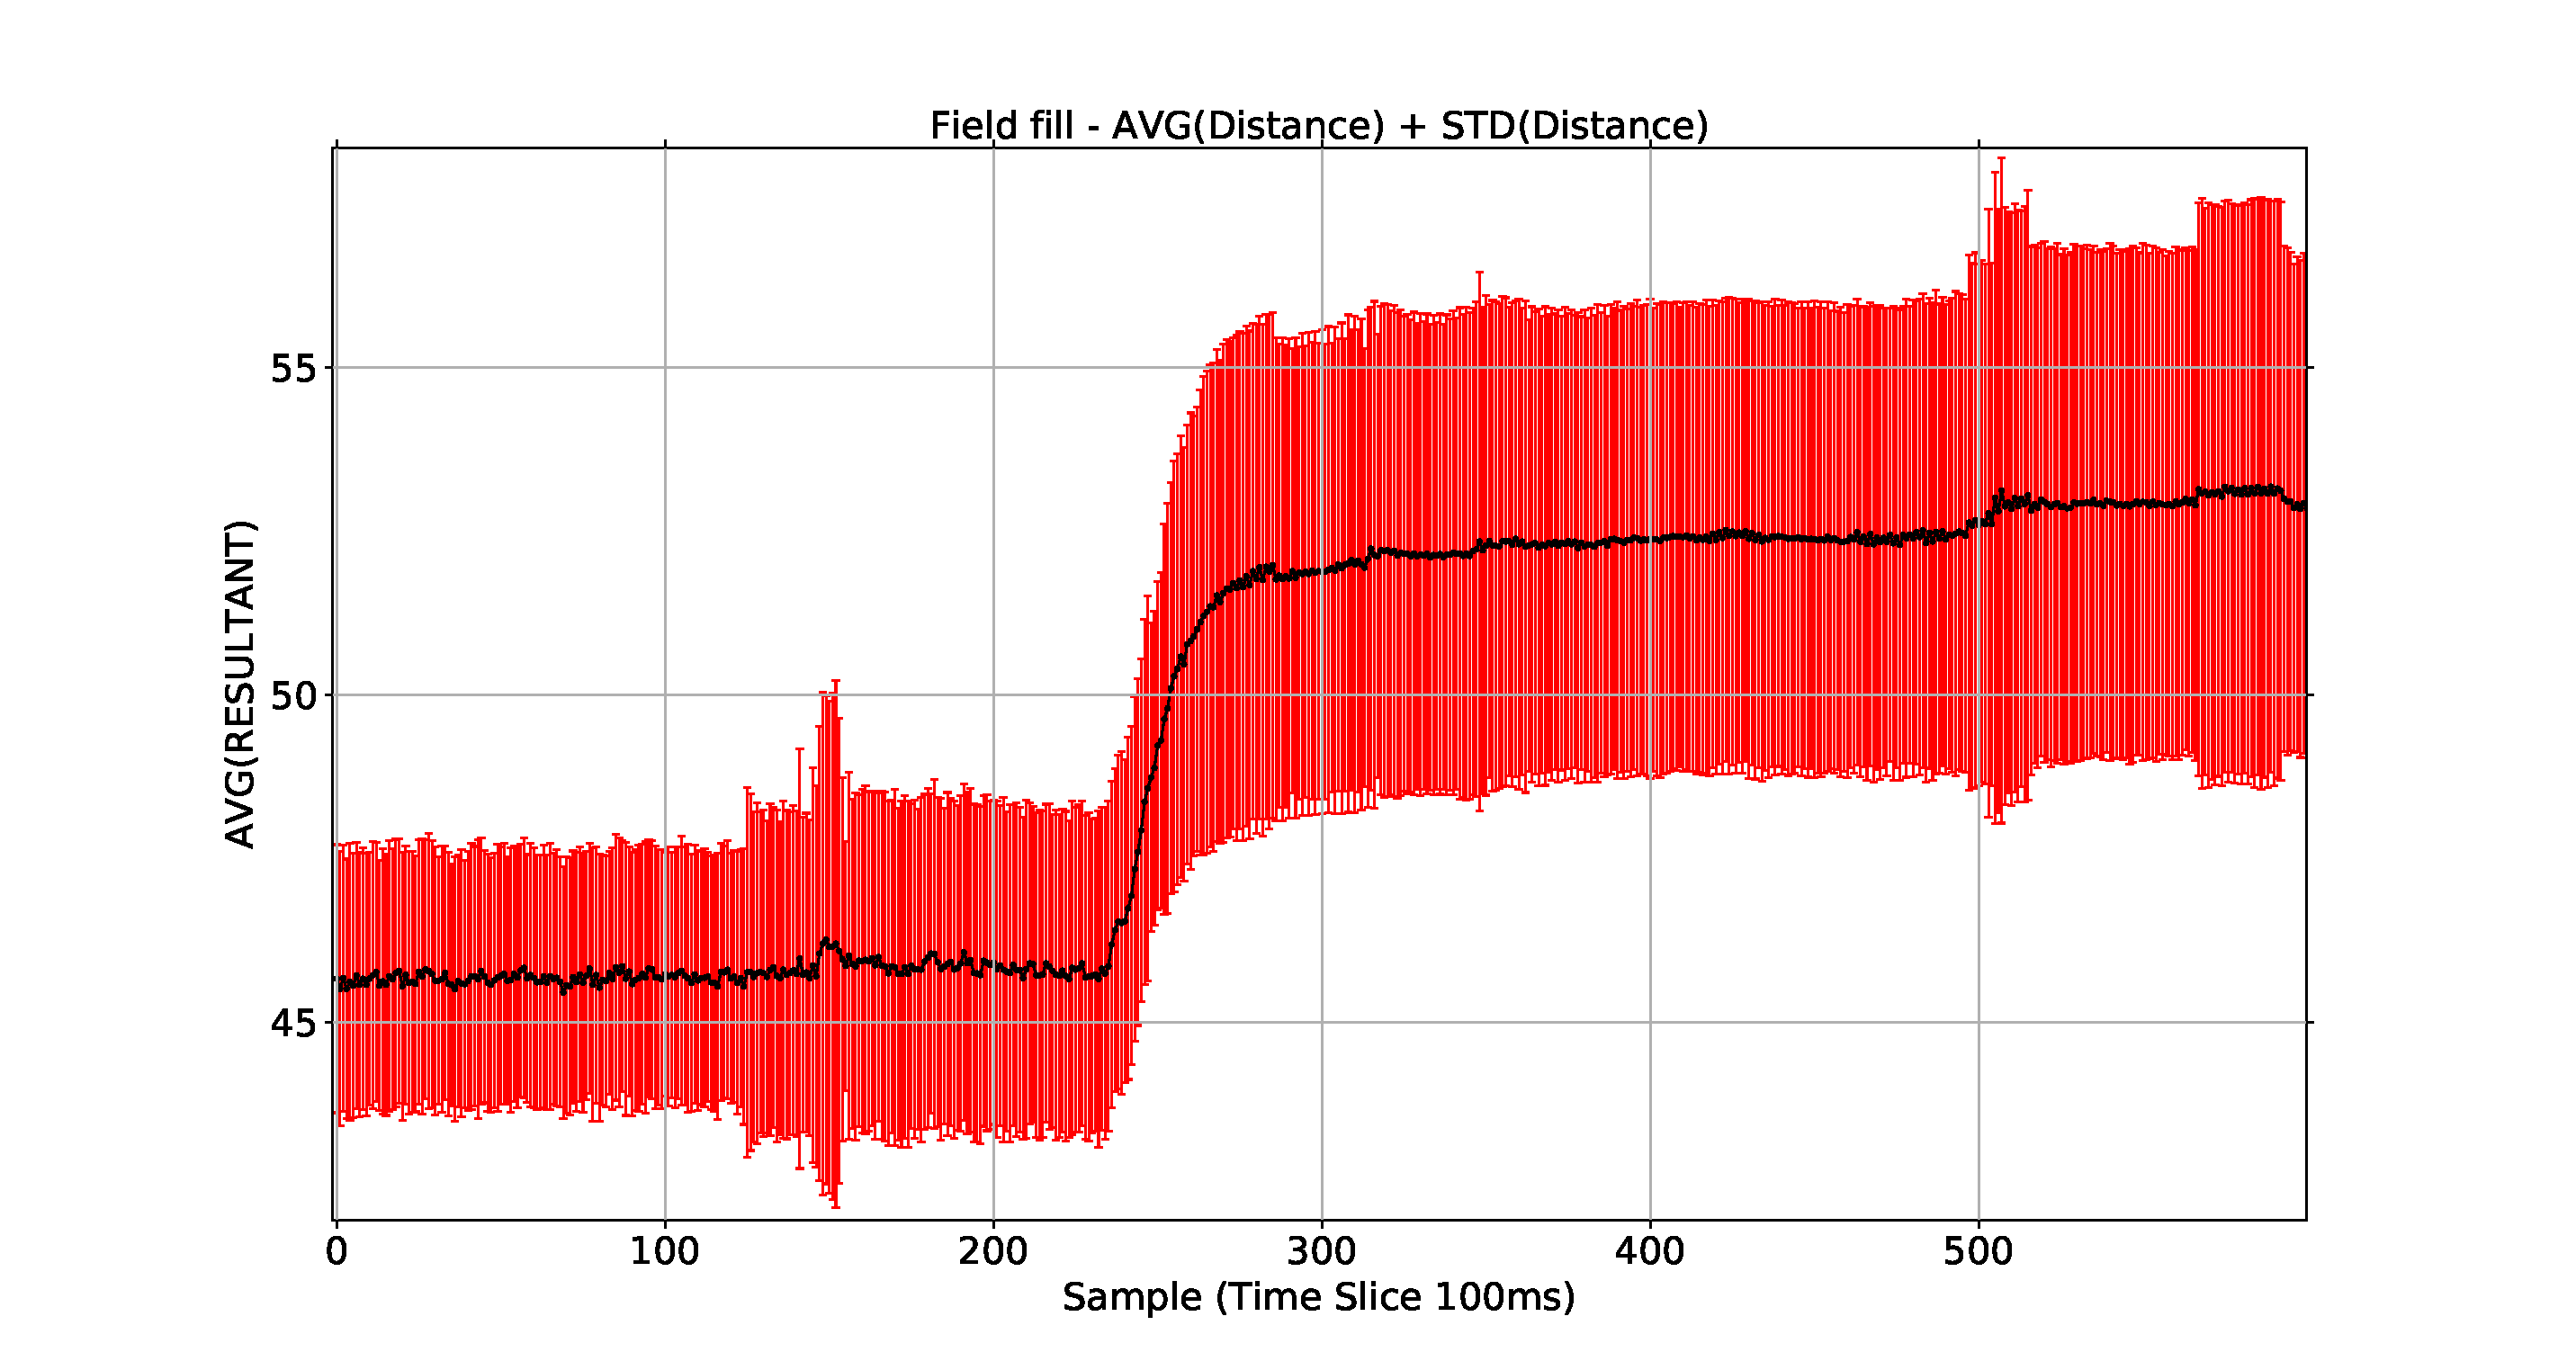
\includegraphics[width=8.5cm]{figures/FIELDFILL-DIST-1}
\end{center}
\caption{Distance metric 0-60 seconds\label{emerge:FIELDFILL-DIST-1}}
\end{figure}

Figure~\ref{emerge:FIELDFILL-DIST-2}~shows the simulation from 60-120 seconds. between 60 and 85 seconds an increment is made in the feild effects and the swarm expands. At 85 seconds there is further increment, however the effect on the distribution is different. The distribution of the agents has changed due to the modality of the swarm. The average distance has increased and there is an increase in the variance. This would indicate that the swam has fully expanded and is unable to expand further. The final increment at 105 seconds can be seen to further impact on the modality indicating the area is saturated.

\begin{figure}
\begin{center}
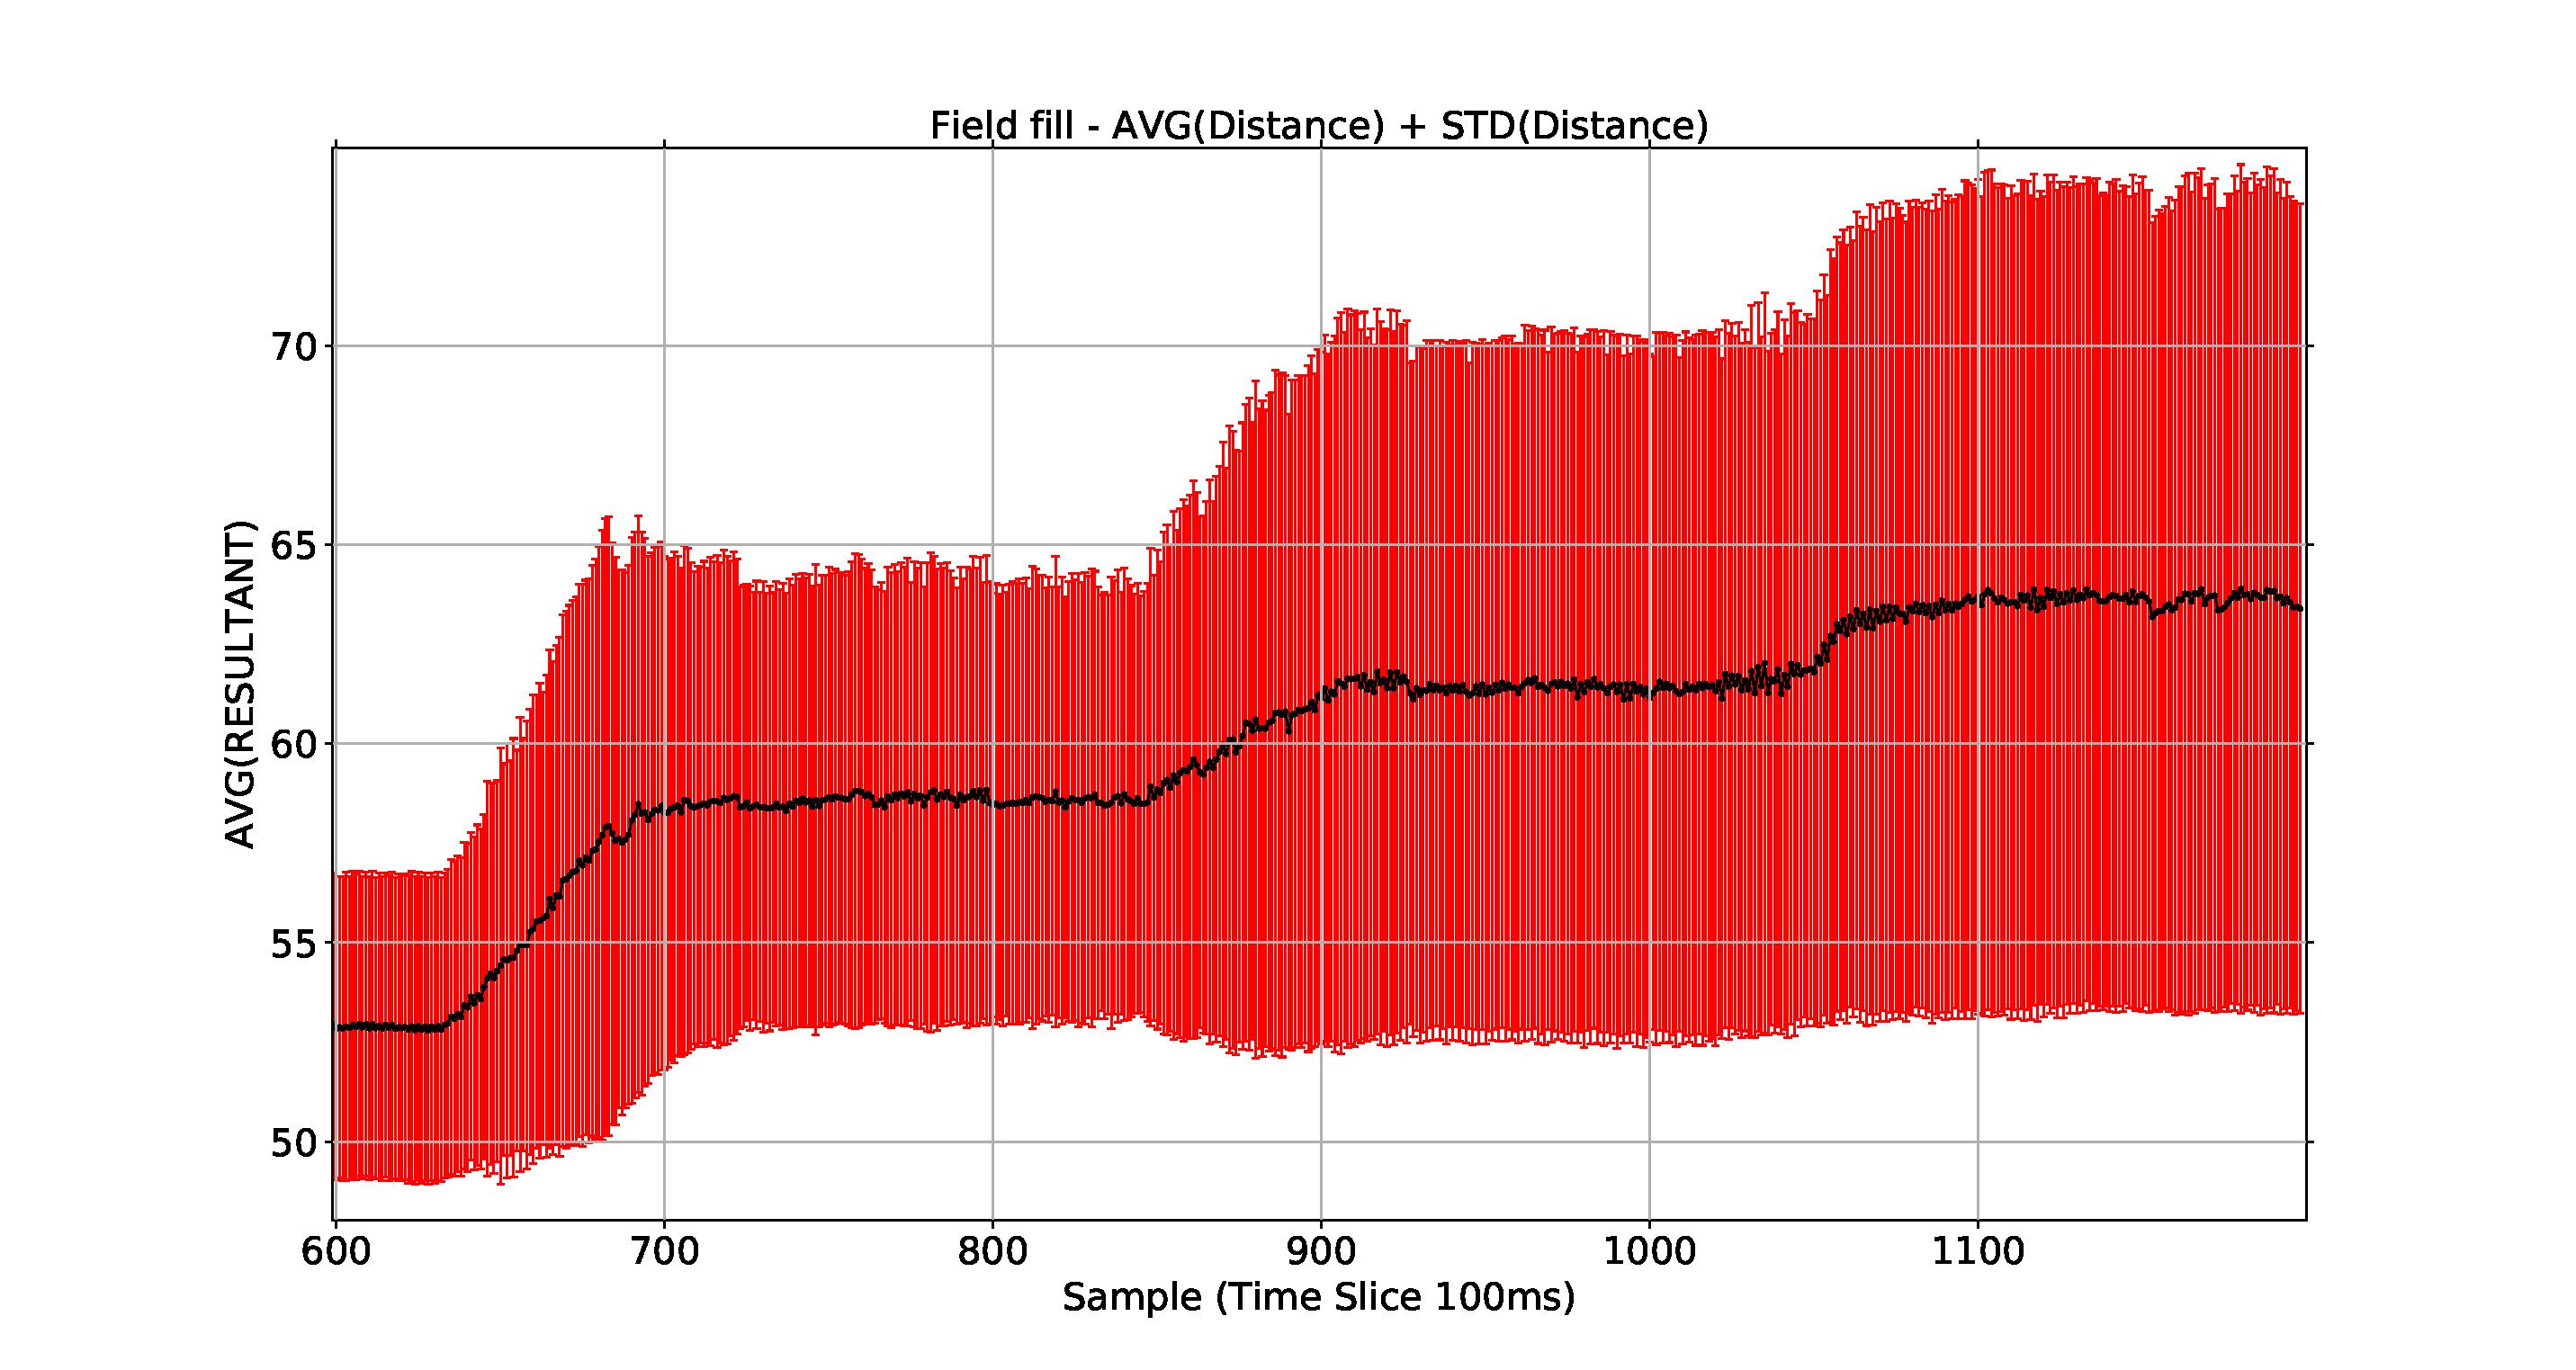
\includegraphics[width=8.5cm]{figures/FIELDFILL-DIST-2}
\end{center}
\caption{Distance metric 60-120 seconds\label{emerge:FIELDFILL-DIST-2}}
\end{figure}

\subsection{Combined magnitude and distance analysis}
Combining the results of the distance and \textit{inter-agent magnitude} metrics provides a more indepth view of the effects changing the field effects has upon the swarms structure.

There is a significant change in the \textit{inter-agent magnitude} when the field effects are incremented to 70 units for repulsion and 80 units for neighbour distance~(Figures \ref{emerge:FIELDFILL-MAG-3} and \ref{emerge:FIELDFILL-MAG-3b}). There is no significant change in the inter-agent distances~(Figures \ref{emerge:FIELDFILL-DIST-3} and \ref{emerge:FIELDFILL-DIST-3b}). Until this point the average \textit{inter-agent magnitude} is positive which indicates an aggregate cohesion in the swarm. After the increment there is an aggregate repulsion in the swarm indicating the swarm is being compressed and the repulsion field effect vector magnitude is greater than the cohesion field effect vector magnitude. A positive cohesion does not indicate the space is not filled only that the swarm still shows a tendency to remain a cohesive entity.

\begin{figure}
\begin{center}
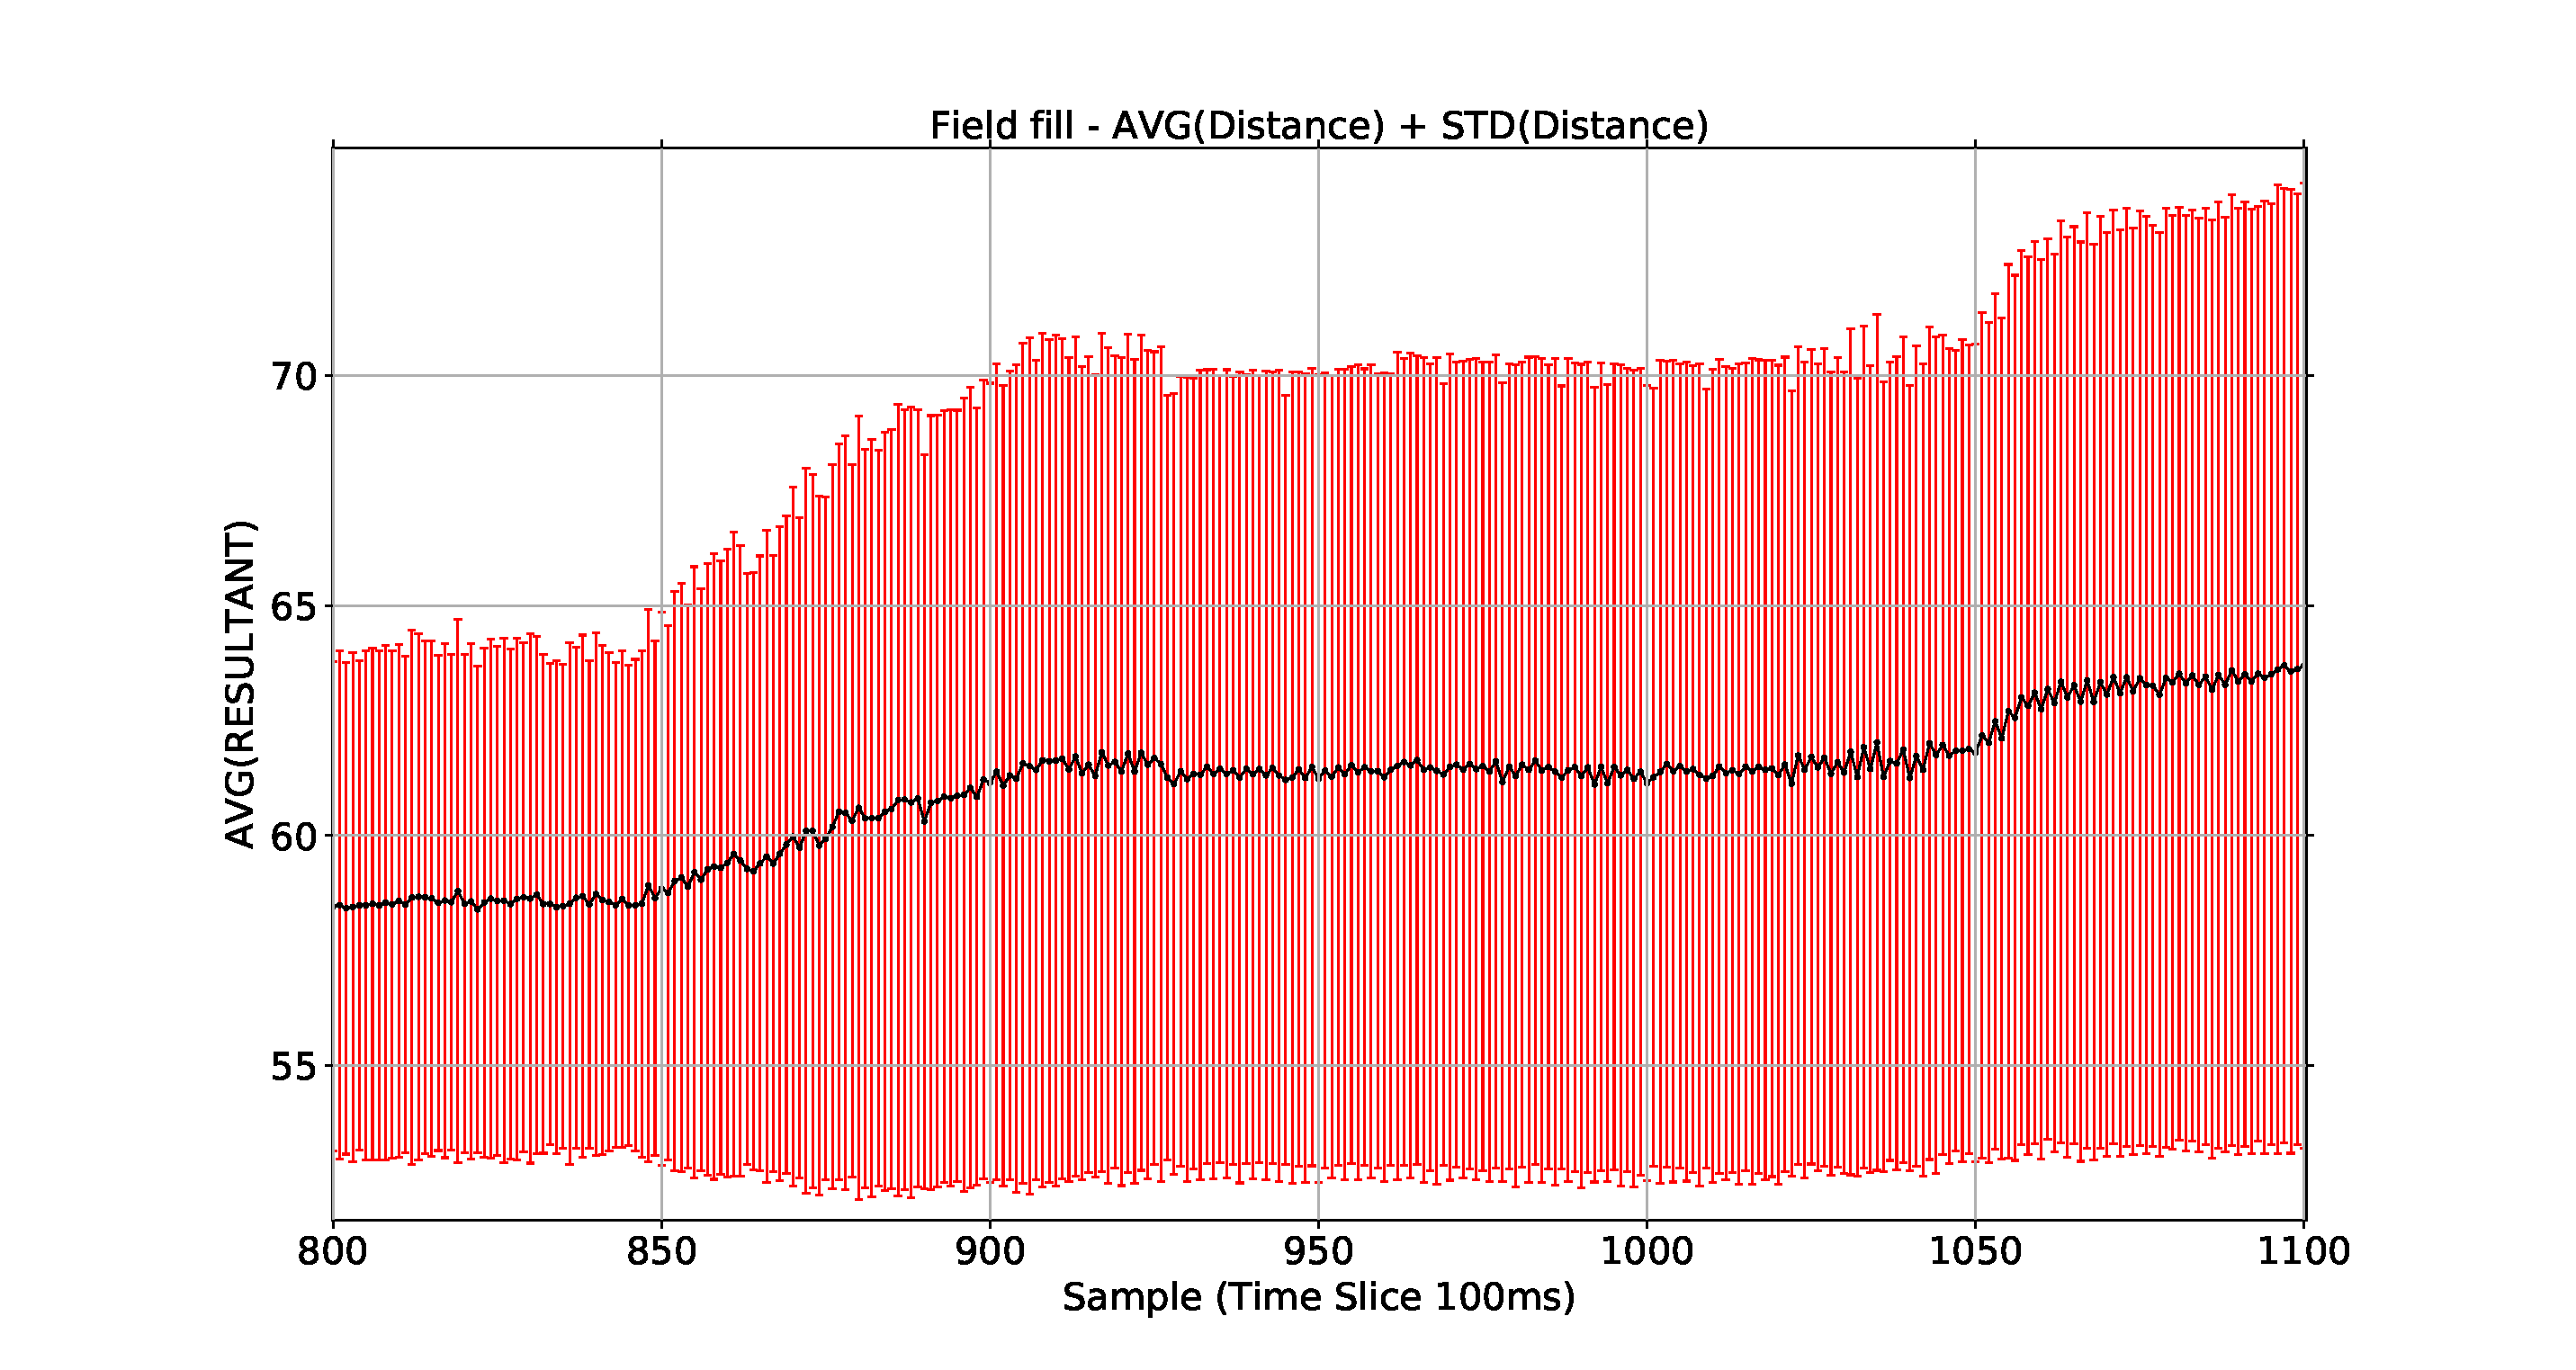
\includegraphics[width=8.5cm]{figures/FIELDFILL-DIST-3}
\end{center}
\caption{Distance metric 80-110 seconds\label{emerge:FIELDFILL-DIST-3}}
\end{figure}

\begin{figure}
\begin{center}
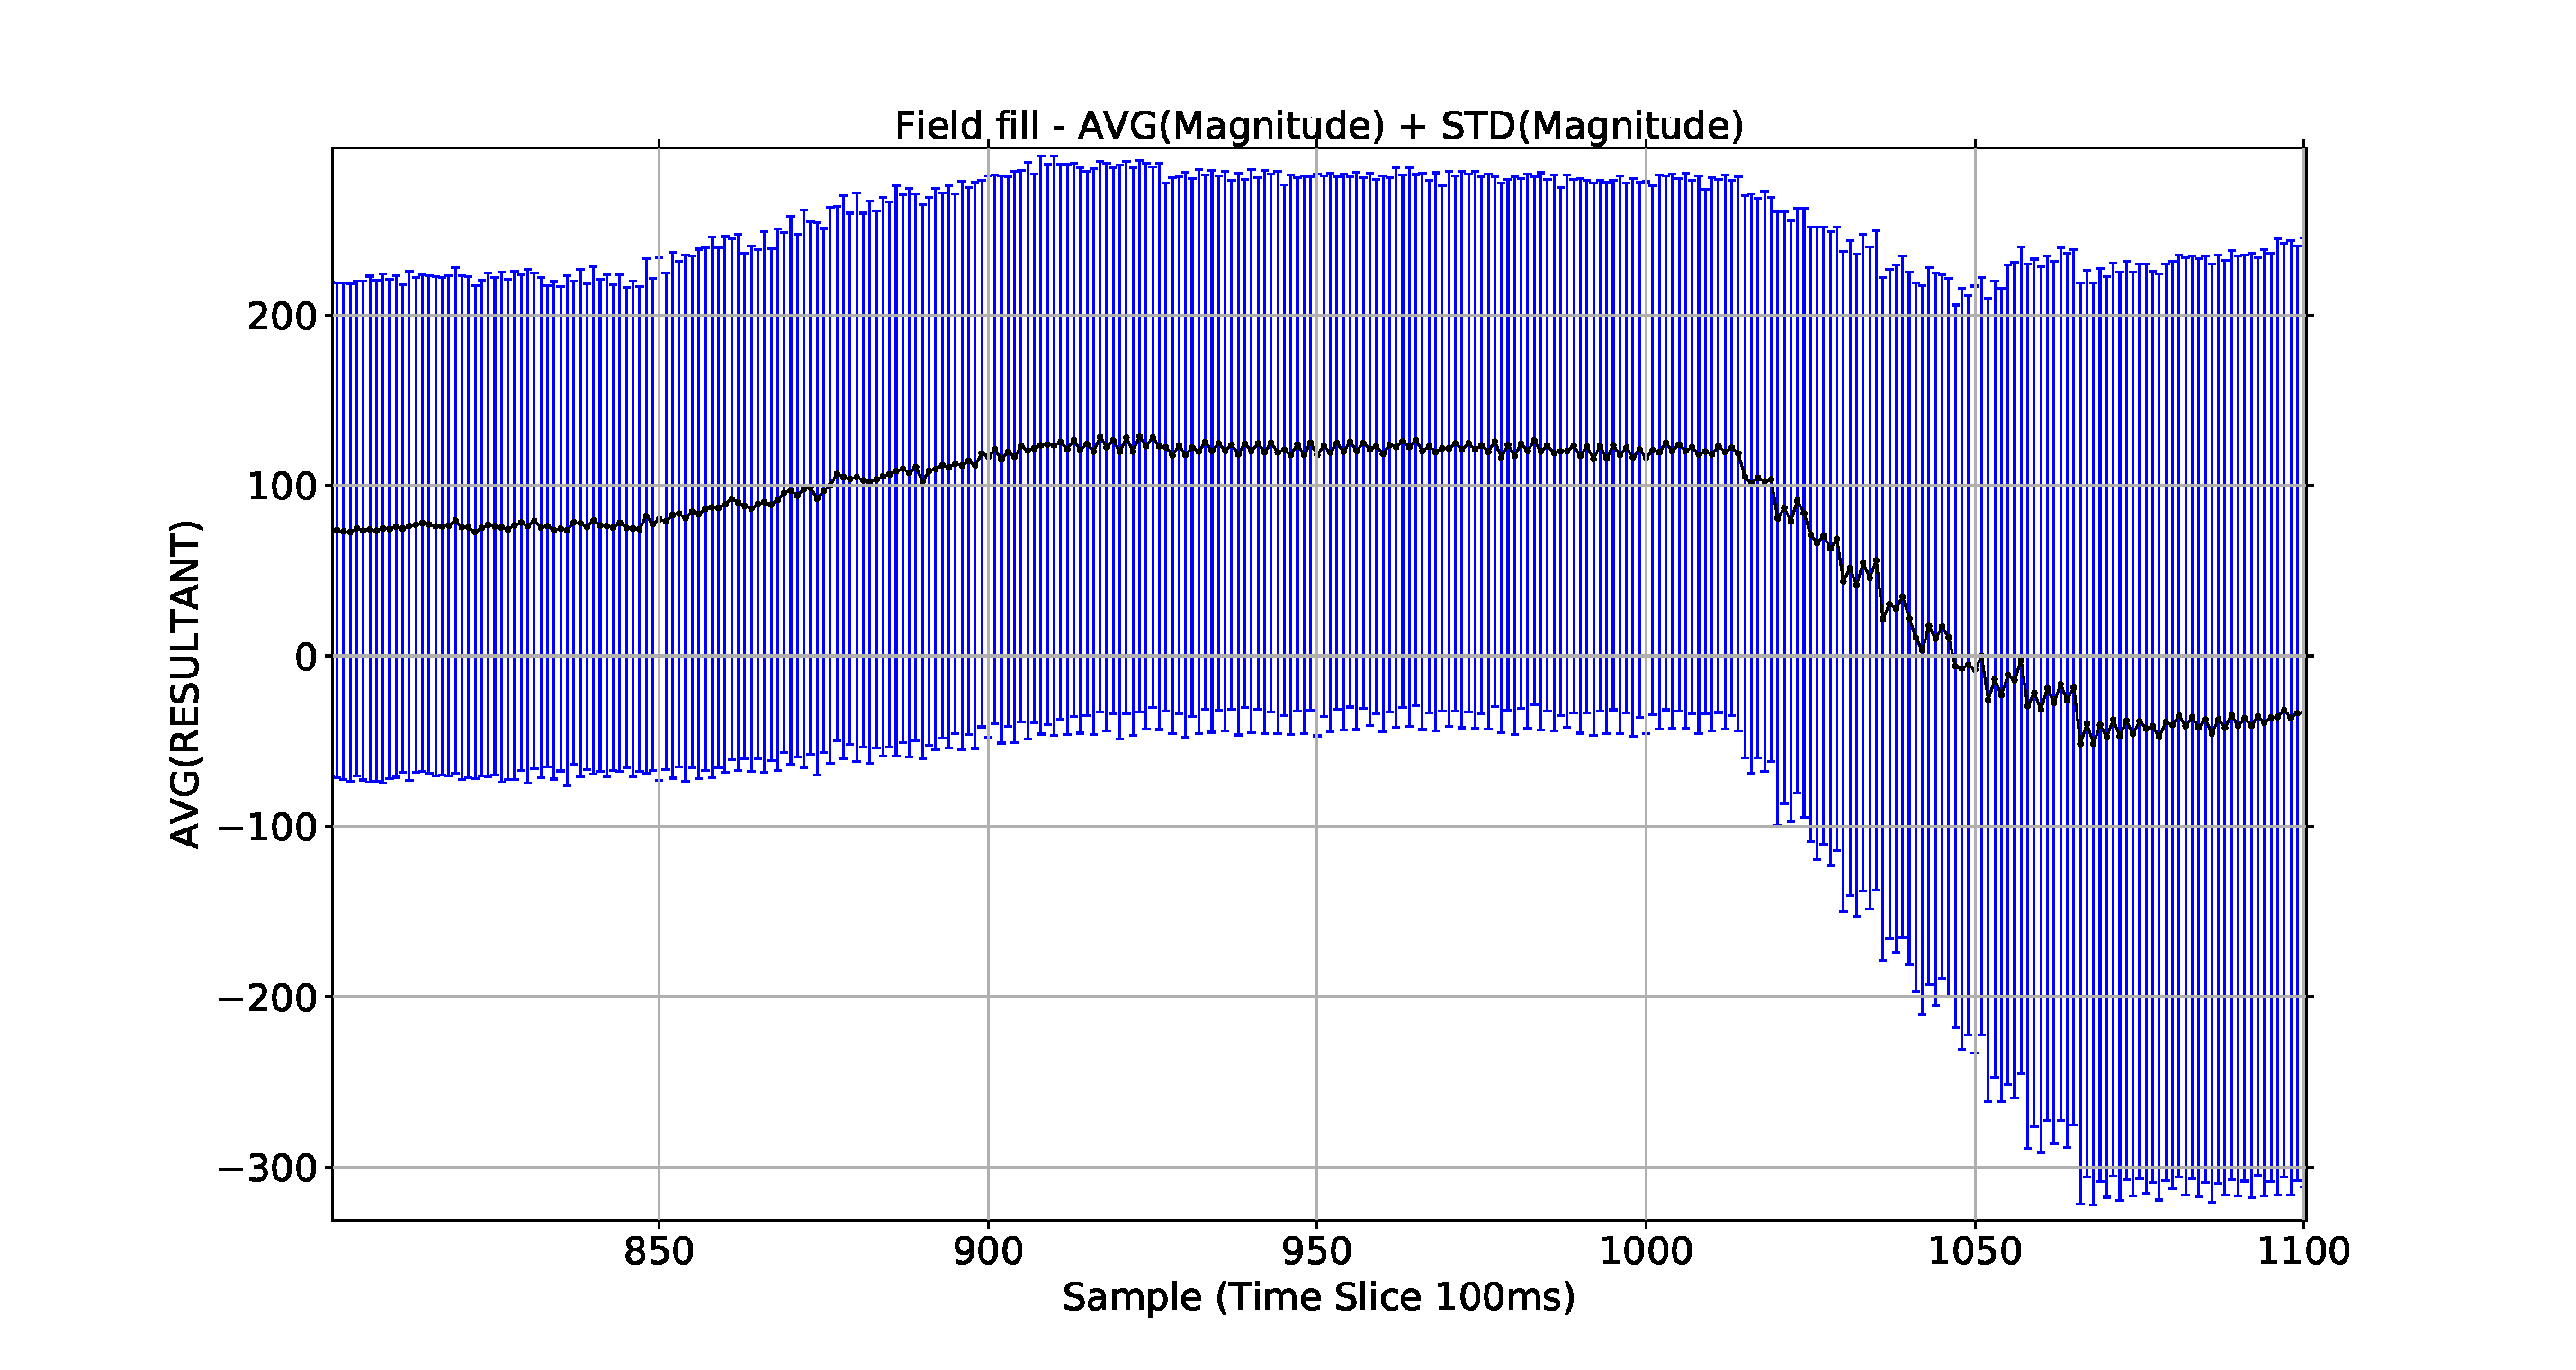
\includegraphics[width=8.5cm]{figures/FIELDFILL-MAG-3}
\end{center}
\caption{Magnitude metric 80-110 seconds\label{emerge:FIELDFILL-MAG-3}}
\end{figure}

\begin{figure}
\begin{center}
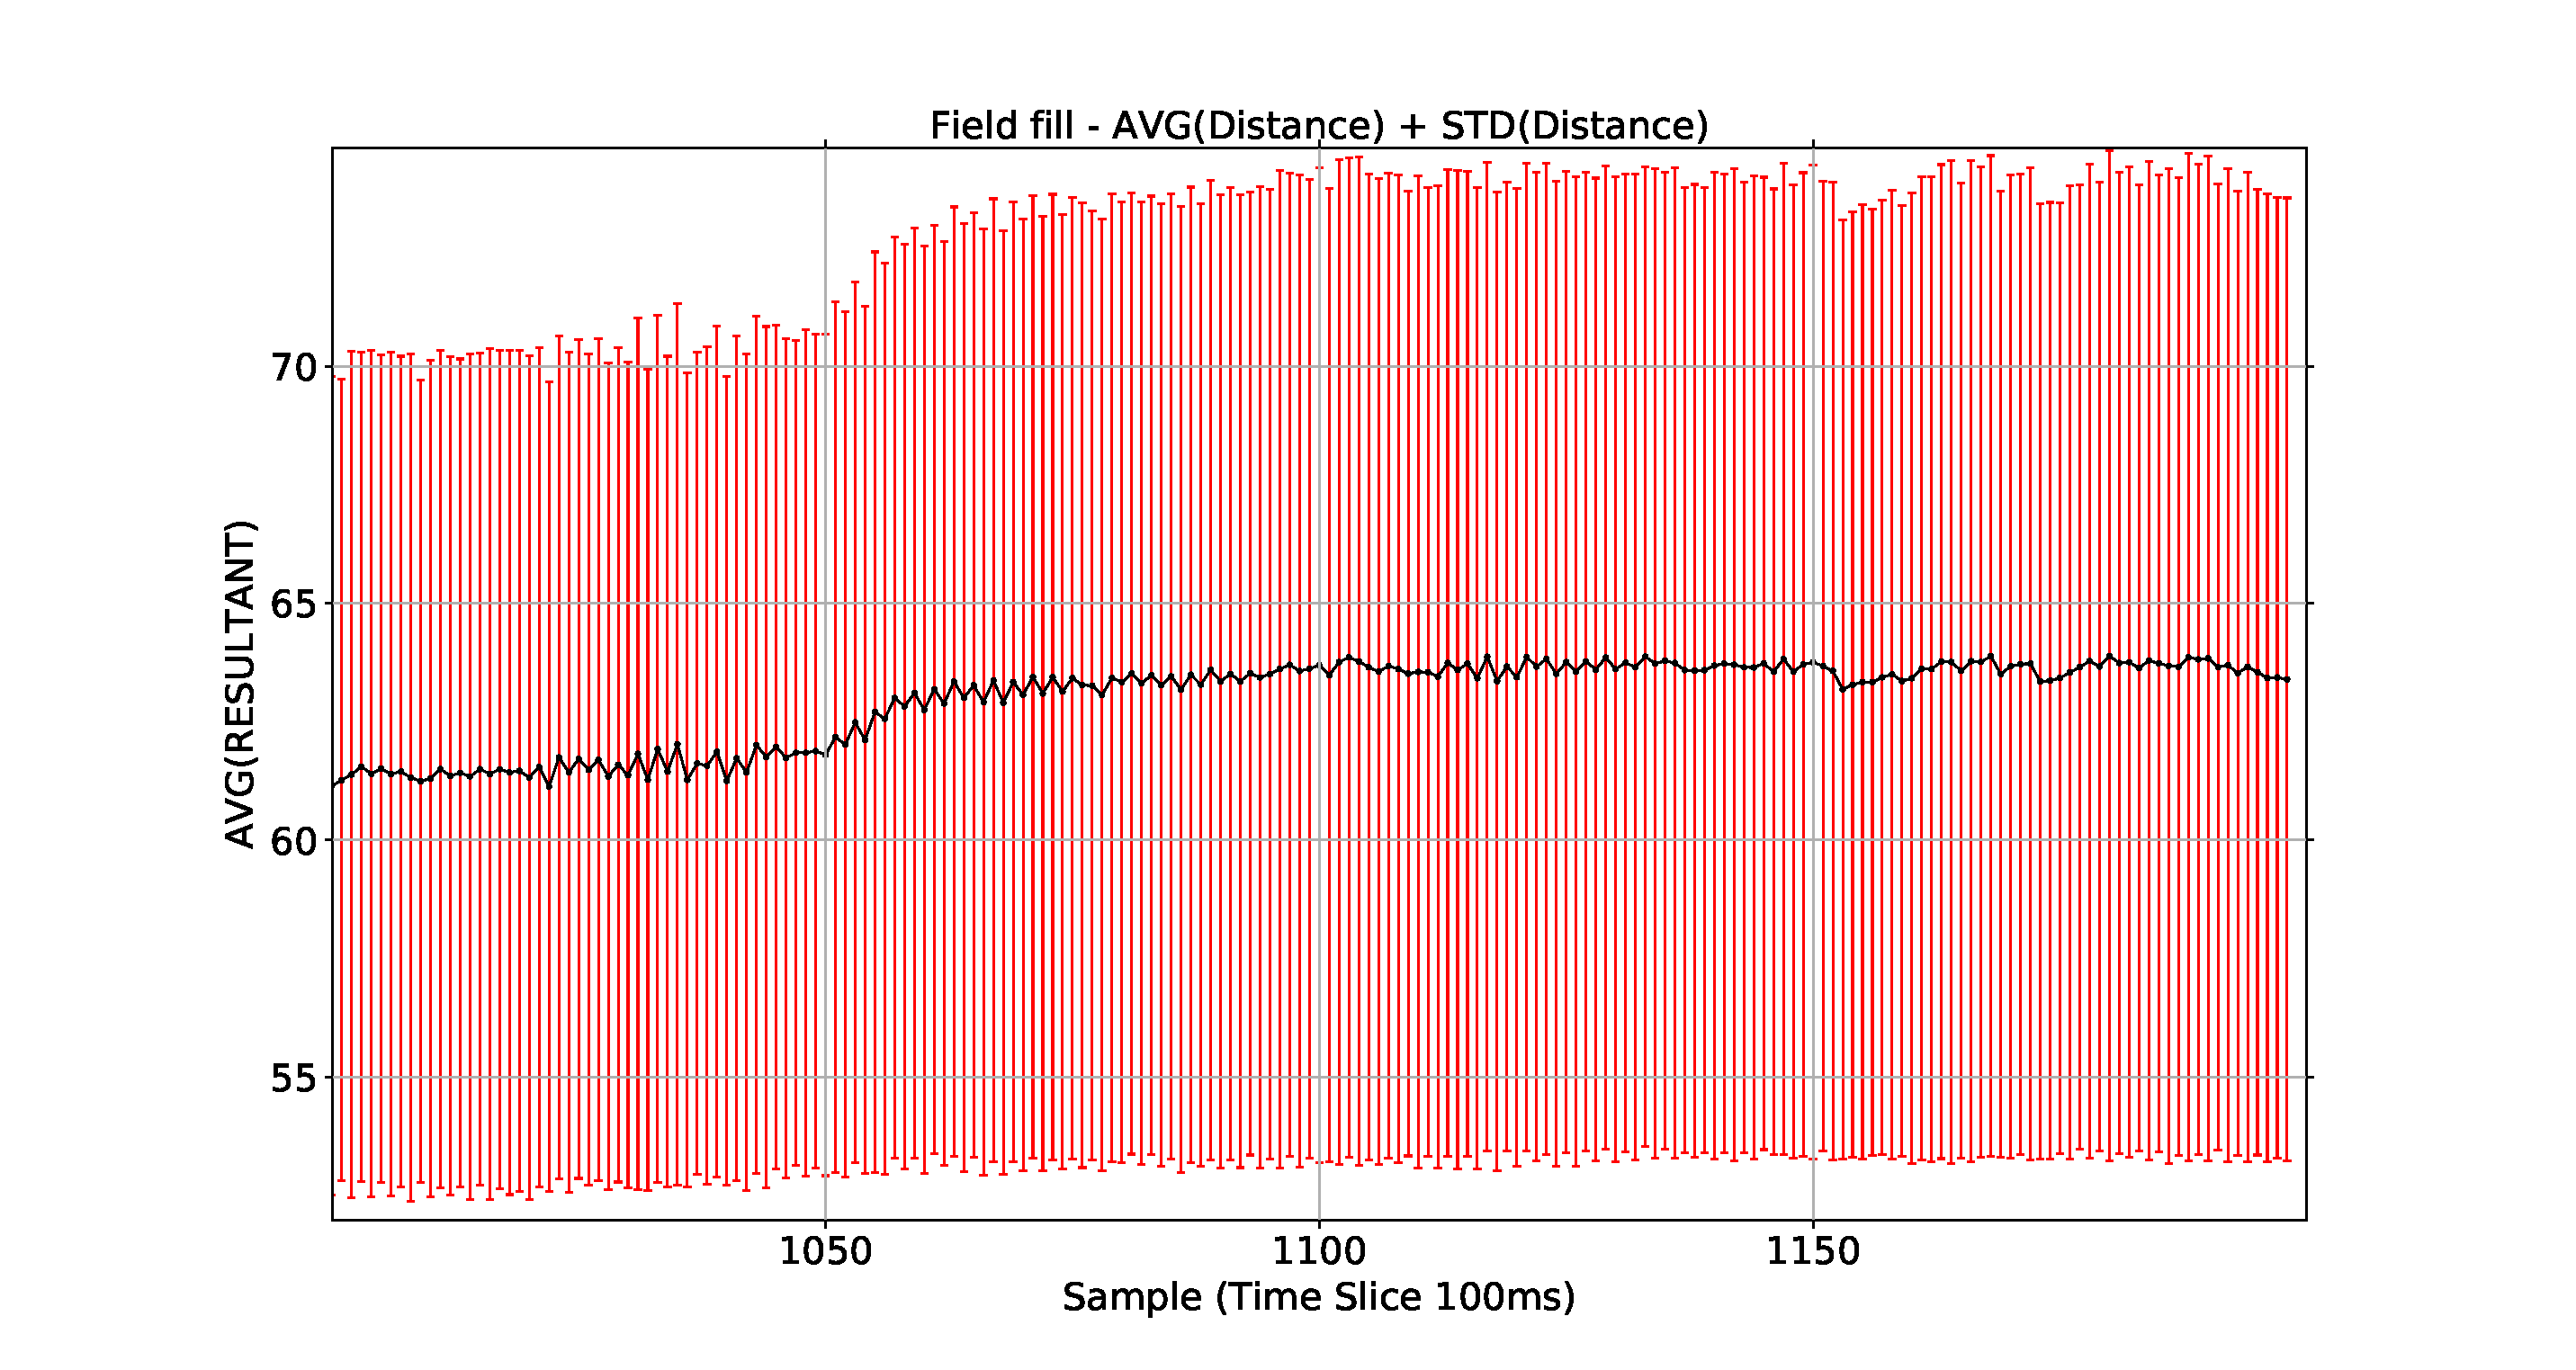
\includegraphics[width=8.5cm]{figures/FIELDFILL-DIST-3b}
\end{center}
\caption{Distance metric 100-120 seconds\label{emerge:FIELDFILL-DIST-3b}}
\end{figure}

\begin{figure}
\begin{center}
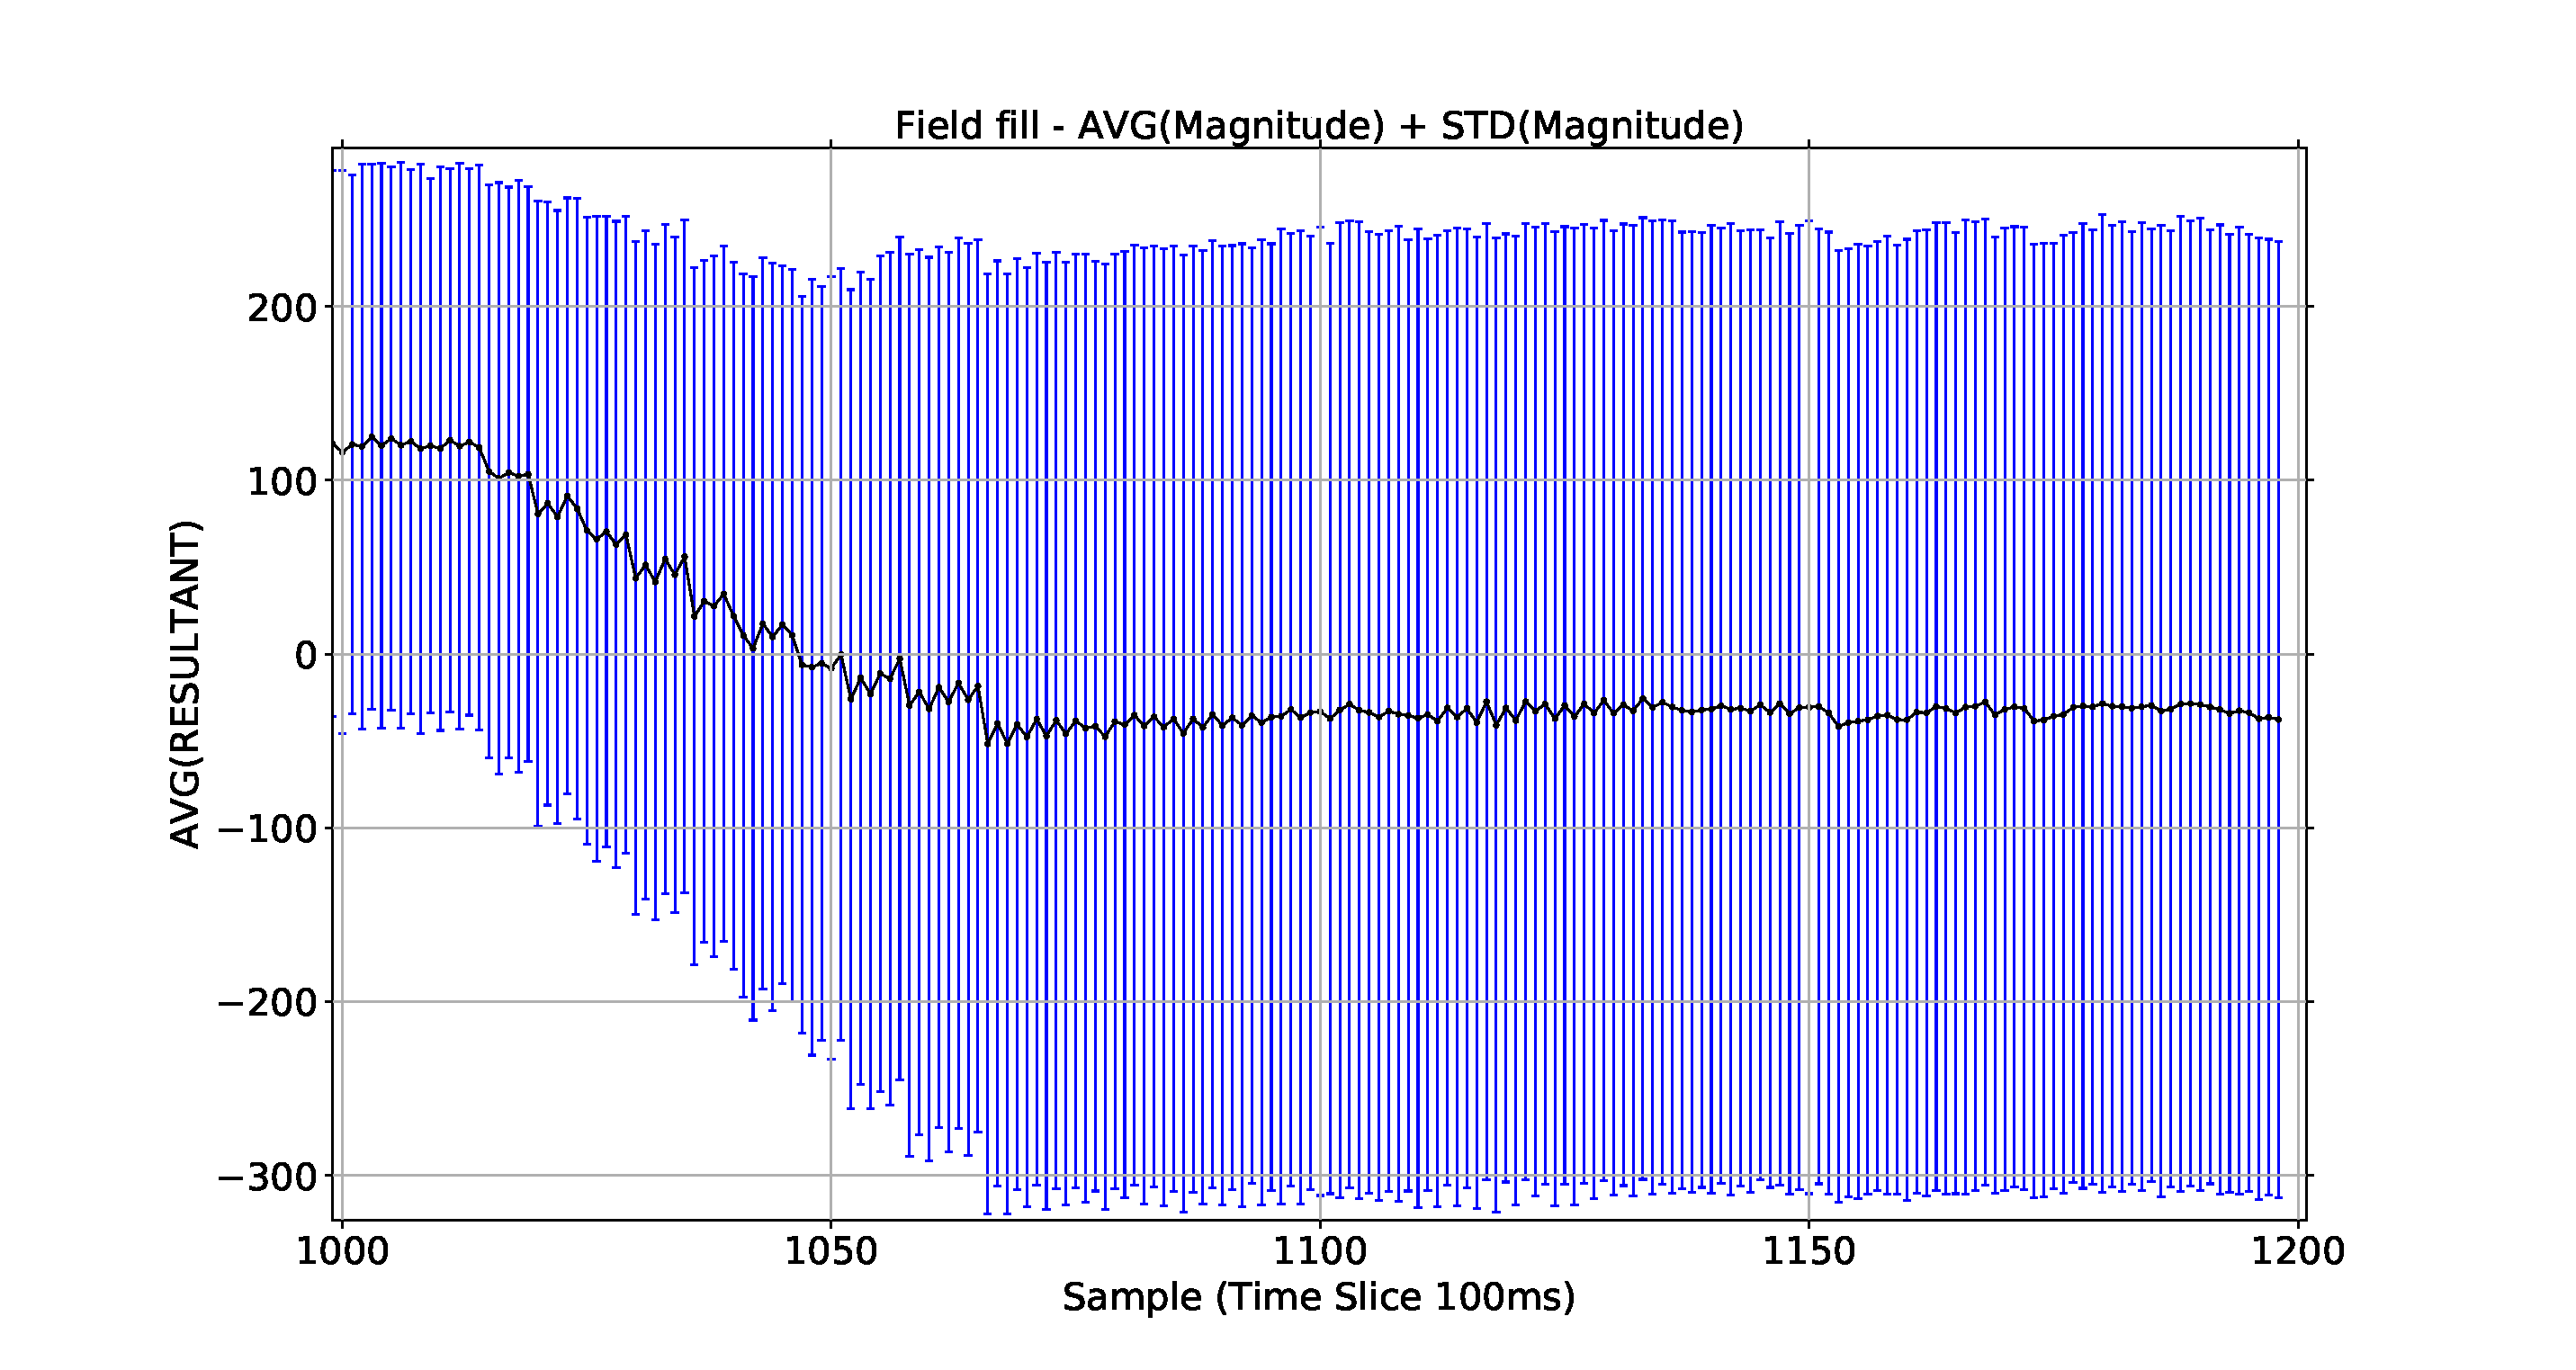
\includegraphics[width=8.5cm]{figures/FIELDFILL-MAG-3b}
\end{center}
\caption{Magnitude metric 100-120 seconds\label{emerge:FIELDFILL-MAG-3b}}
\end{figure}

\section{Field effect modification with repulsion only}
The previous mechanism for area filling uses a swarm that utilising both repulsion and cohesion to ensure the swarm remains, as far as is possible, a single entity. When using repulsion only it is accepted that the agents are in a restricted area and not being cohesive is not and issue as the field effects can be expanded until the agents interact with each other and the boundary. A similar approach was used by Scheutz and Bauer in 2006~\cite{SB:06}. The repulsion field effect in this paper is used with a fixed sized swarm and the repulsion field is increase over time. The simulation for this experiment uses 52 agents in the same confined space as the previous experiment. The parameters are shown below: 

\begin{table}
\begin{center}
\begin{tabular}{| p{1.5cm} | p{1.5cm} | p{4.0cm} |}
\hline
\bf Parameter & \bf Value  & \bf Description \\ \hline
$k_c$         & 0          & weight adjuster for cohesion vector\\ \hline
$k_r$         & 15         & weight adjuster for repulsion vector\\ \hline
Sample rate   & 100 ms      & proximity sensor rate\\ \hline
Speed         & 20 units/s & agent speed\\ \hline
\end{tabular}\caption{Swarm parameters repulsion only} \label{tab:FillParameters}
\end{center}
\end{table}

\begin{table}
\begin{center}
%\begin{tabular}{| p{2cm} | p{0.5cm} | p{0.5cm} | p{0.5cm} | p{0.5cm} | p{0.5cm} | p{0.5cm} | p{1cm} |}
\begin{tabular}{| p{1.5cm} | p{0.3cm} | p{0.3cm} | p{0.3cm} | p{0.3cm} | p{0.3cm} | p{0.3cm} | p{0.5cm} |}
\hline
\bf Weight \bf component & \bf 1 & \bf 2 & \bf 3 & \bf 4 & \bf 5 & \bf 6 & \\ \hline
Repulsion Boundary & 50 & 51 & 52 & 53 & 54 & 55 & units\\  \hline
Neighbour Distance & 70 & 70 & 70 & 70 & 70 & 70 & units\\  \hline
\end{tabular}\caption{field effect expansion sequence} \label{tab:BaselineConcaveReduction}
\end{center}
\end{table}

The theory behind this type of flood filling is as follows; Cohesion and repulsion acting against each other causes jitter, removing the cohesion allows the swarm to expand to its maximum volume with all agents distributed so they no longer interact at which point jitter will cease. The boundary created by the enclosed space will effect the expanding swarm by repelling the agents back into the swarm preventing expansion therefore the swarm movement will propogate to fill vacant areas. Jitter will initially be seen as the swarm equalises and it will decrease to zero when the swarm is fully expanded. There will be a point in the swarms expansion when the agents will not be able to extend to a zero repulsion point and there will be a permanent interaction between the perimeter and agents. This condition is the exit point for the repulsion flood fill.

Figures~\ref{emerge:Repel52-1}, \ref{emerge:Repel52-2}, \ref{emerge:Repel52-3}, \ref{emerge:Repel52-4}, \ref{emerge:Repel52-5} and \ref{emerge:Repel52-6} show the stages that a field-repulsion-area-fill propagates through. The initial deployment is shown in~Figure~\ref{emerge:Repel52-1}. When the simulation starts the swarm immediately expands~(Figure~\ref{emerge:Repel52-2}) and all the agents stabilise to a position where thier movement stops. The field effect is increased and the swarm distribution movement commences. This cycle continues until the swarm is unable to resolve to a neutral expansion point.

\begin{figure}
\begin{center}
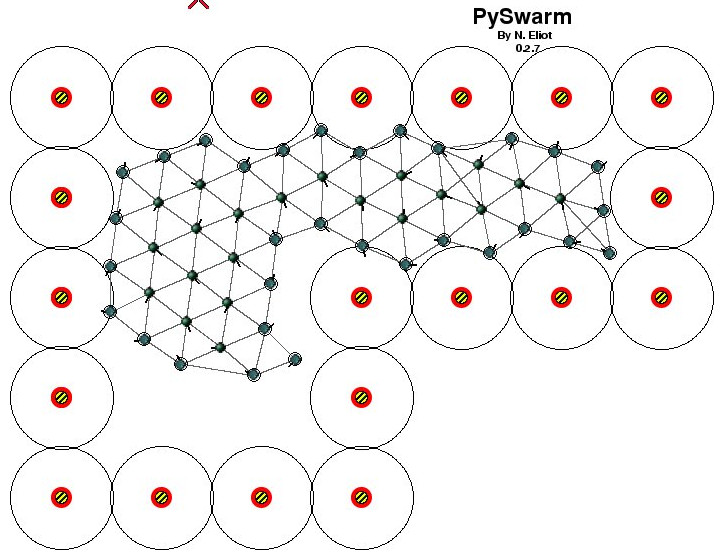
\includegraphics[width=5.5cm]{figures/REPEL52-1}
\end{center}
\caption{Stage 1\label{emerge:Repel52-1}}
\end{figure}

\begin{figure}
\begin{center}
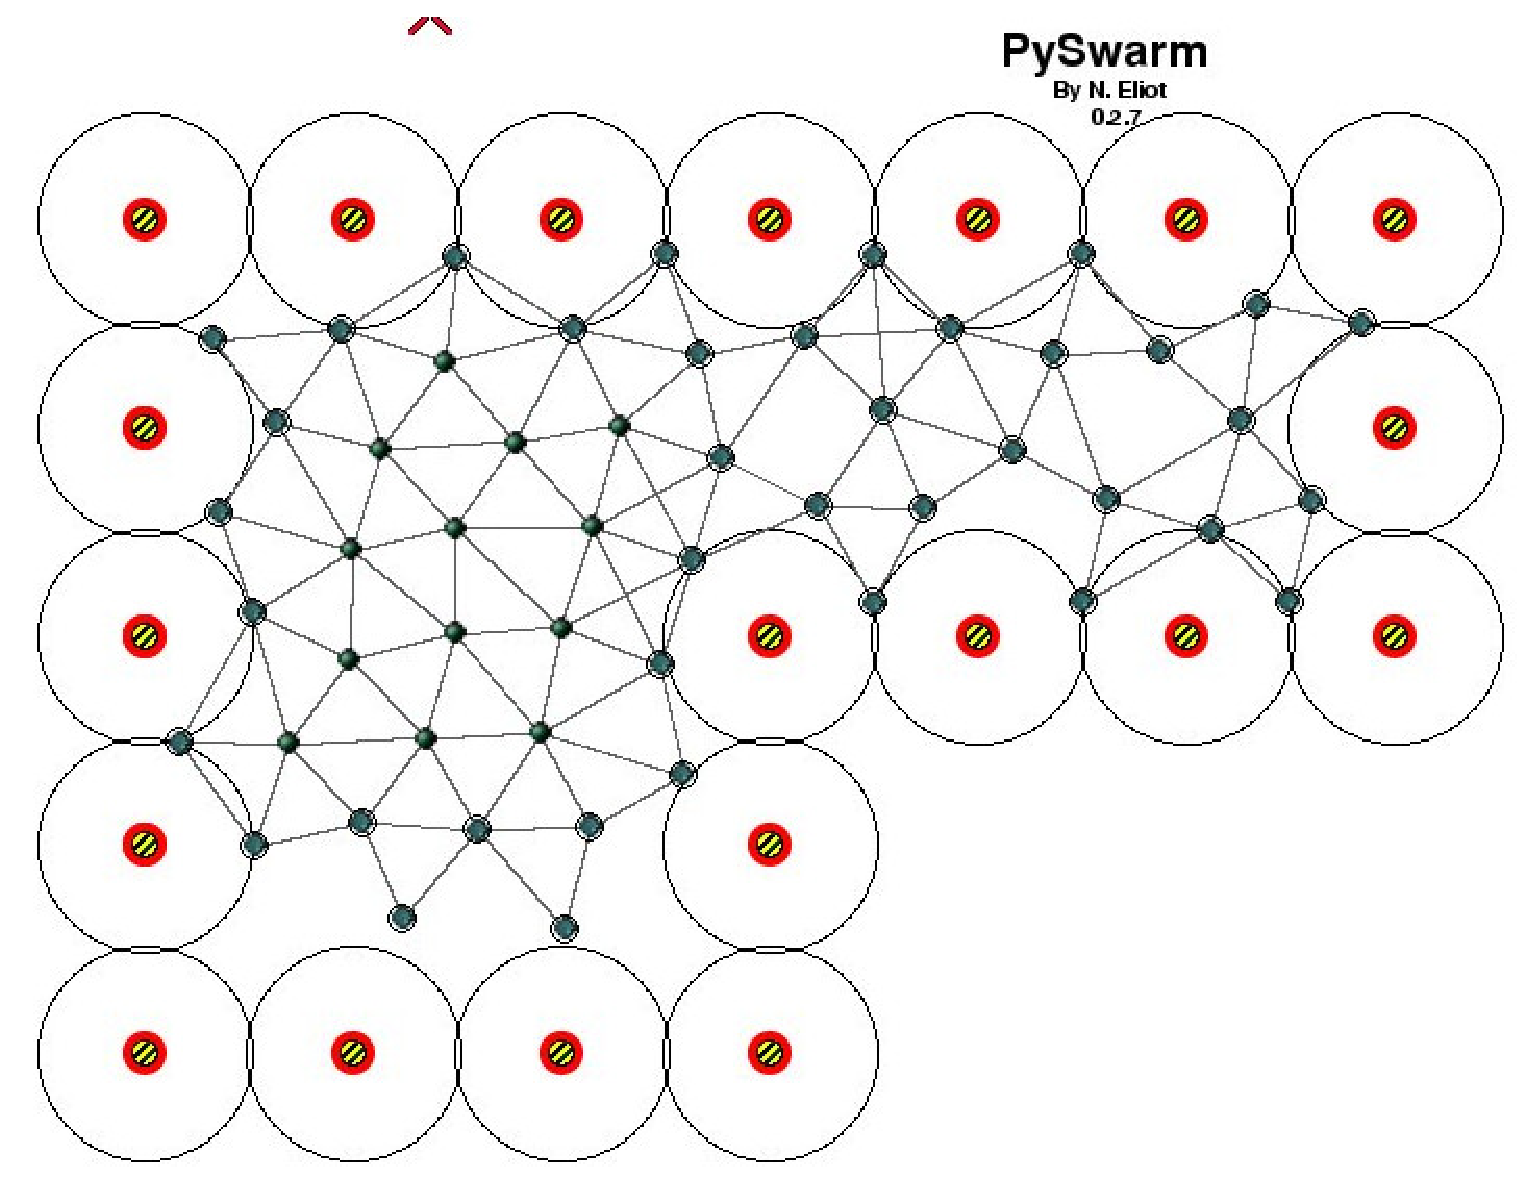
\includegraphics[width=5.5cm]{figures/REPEL52-2}
\end{center}
\caption{Stage 2\label{emerge:Repel52-2}}
\end{figure}

\begin{figure}
\begin{center}
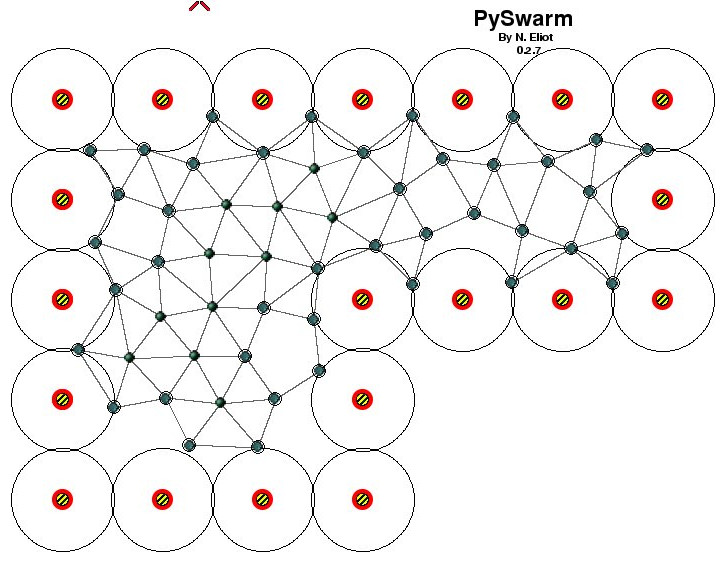
\includegraphics[width=5.5cm]{figures/REPEL52-3}
\end{center}
\caption{Stage 3\label{emerge:Repel52-3}}
\end{figure}

\begin{figure}
\begin{center}
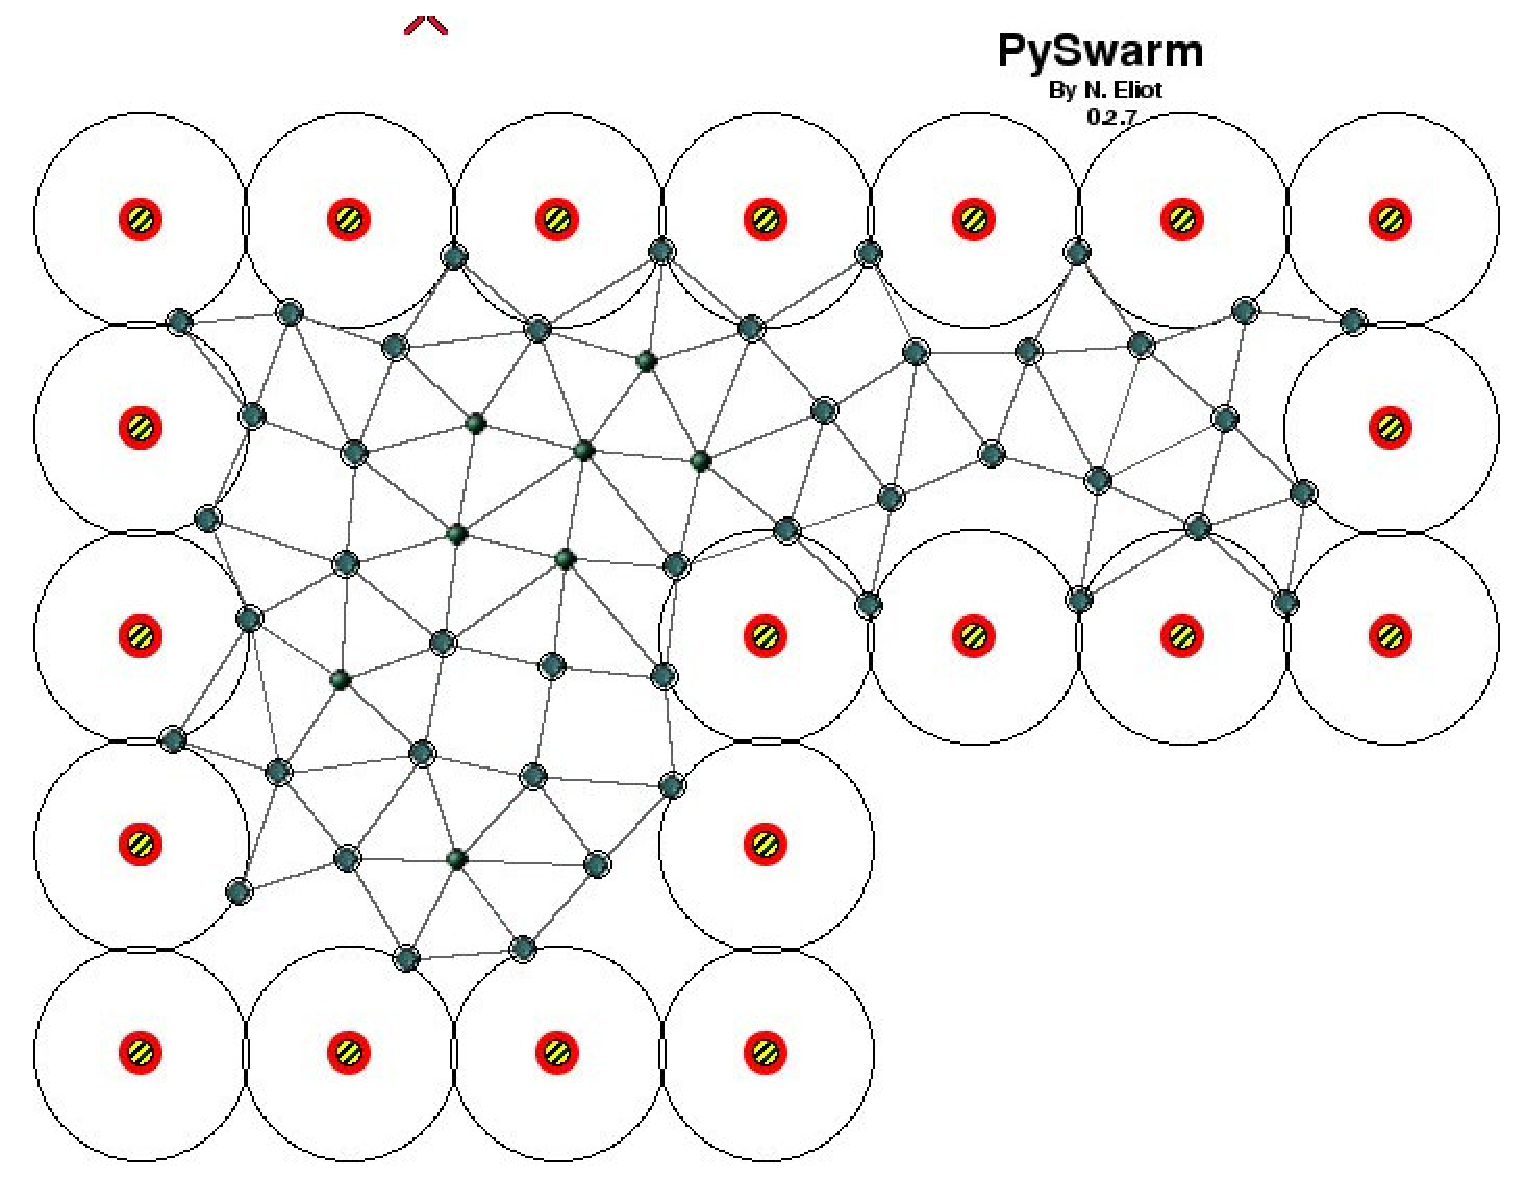
\includegraphics[width=5.5cm]{figures/REPEL52-4}
\end{center}
\caption{Stage 4\label{emerge:Repel52-4}}
\end{figure}

\begin{figure}
\begin{center}
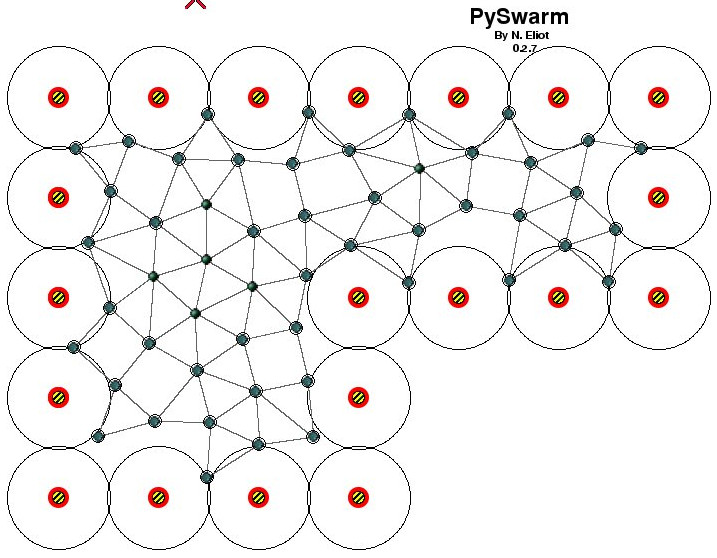
\includegraphics[width=5.5cm]{figures/REPEL52-5}
\end{center}
\caption{Stage 5\label{emerge:Repel52-5}}
\end{figure}

\begin{figure}
\begin{center}
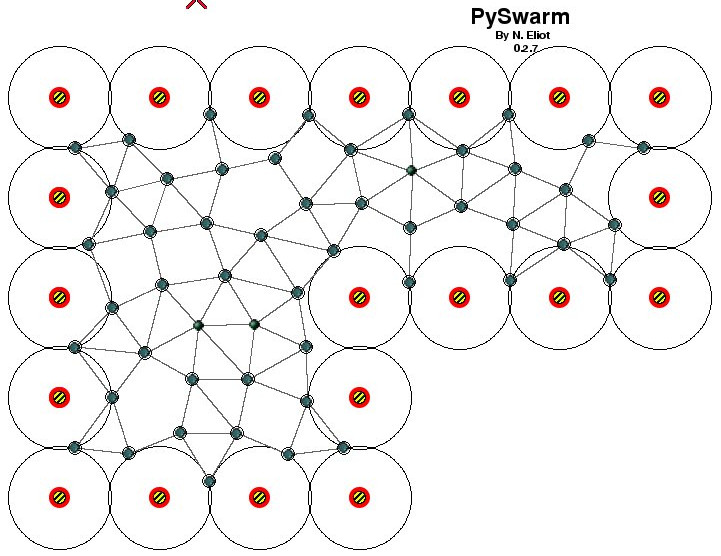
\includegraphics[width=5.5cm]{figures/REPEL52-6}
\end{center}
\caption{Stage 6\label{emerge:Repel52-6}}
\end{figure}


%% \begin{figure}
%% \centering
%% \subfigure[Stage 1]{
%% 	 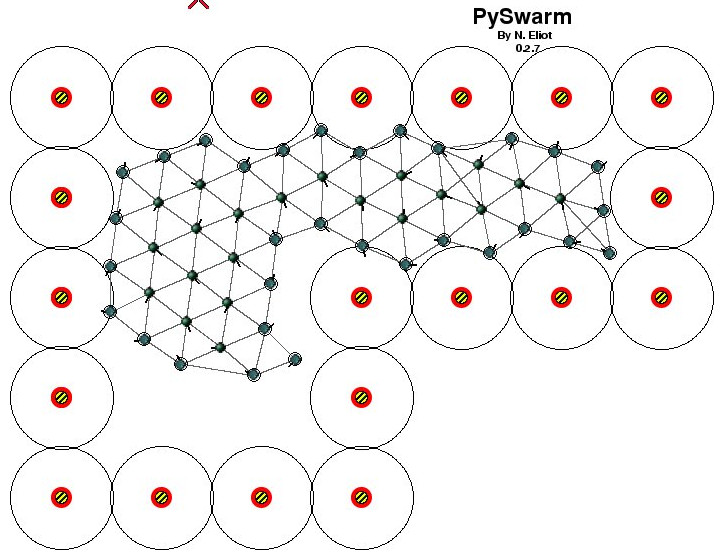
\includegraphics[width=5.5cm]{figures/REPEL52-1}
%% 	 \label{emerge:Repel52-1}
%% }
%% \subfigure[Stage 2]{
%% 	 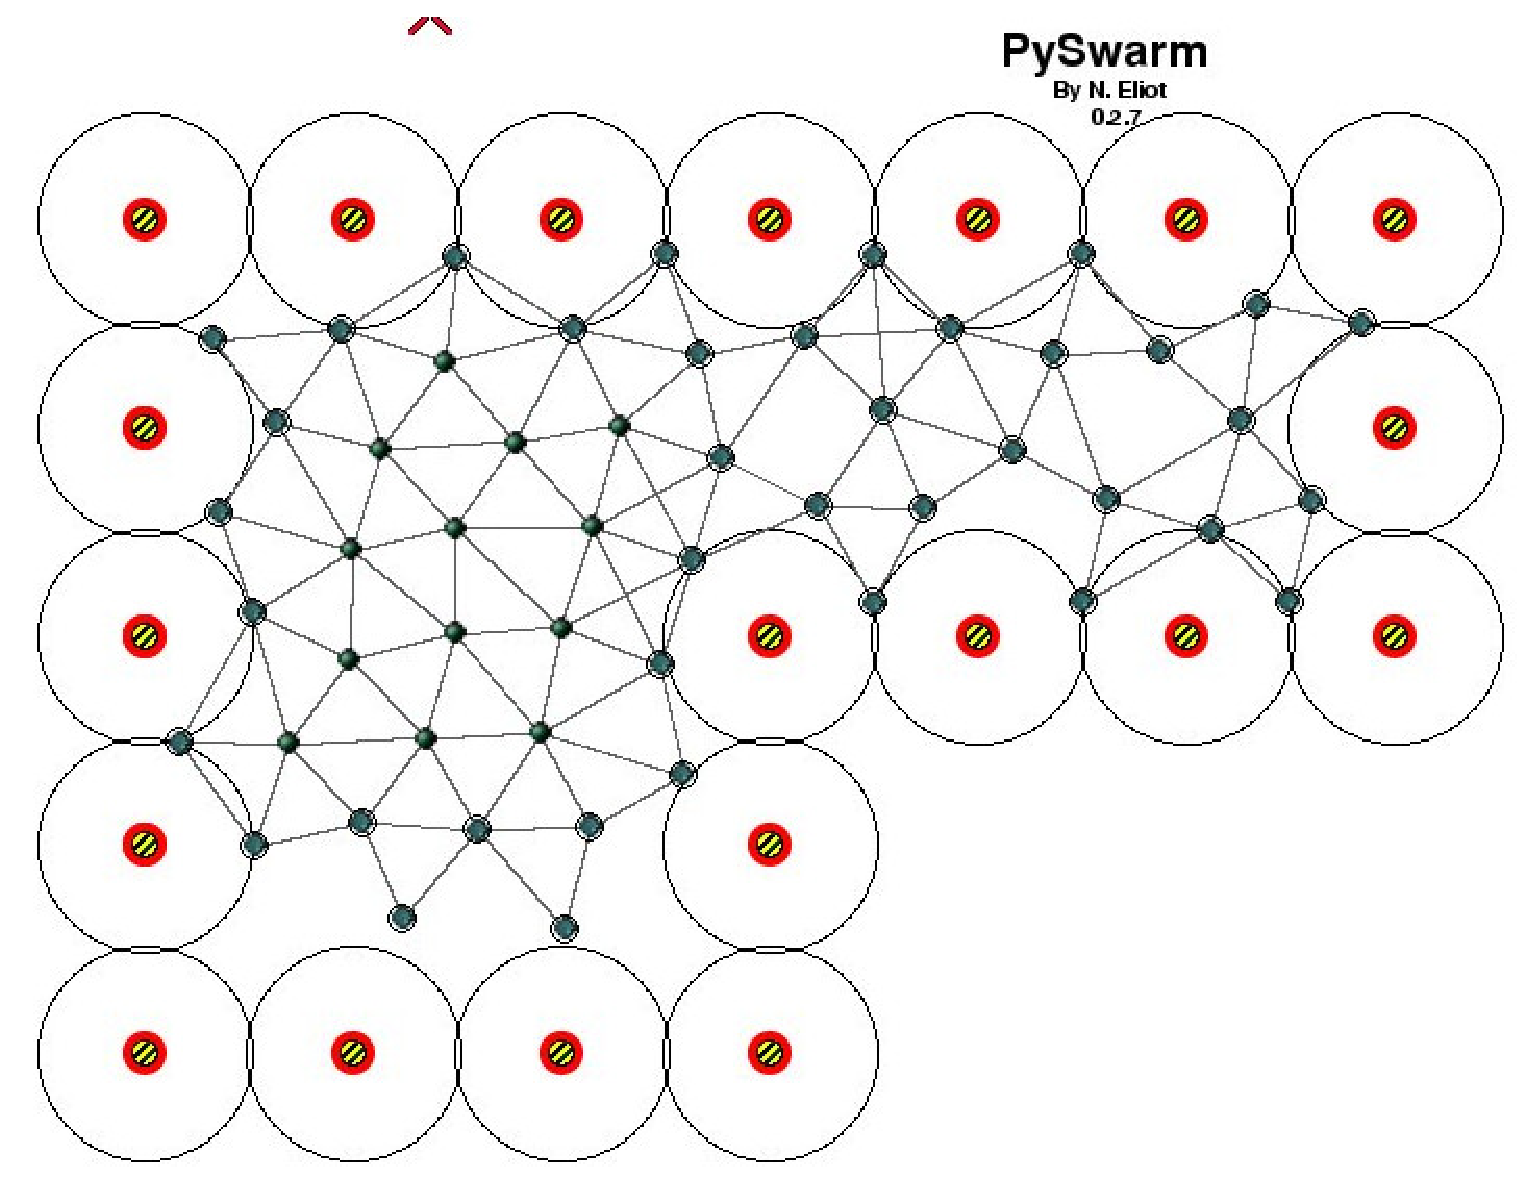
\includegraphics[width=5.5cm]{figures/REPEL52-2}
%% 	 \label{emerge:Repel52-2}
%% }
%% \subfigure[Stage 3]{
%% 	 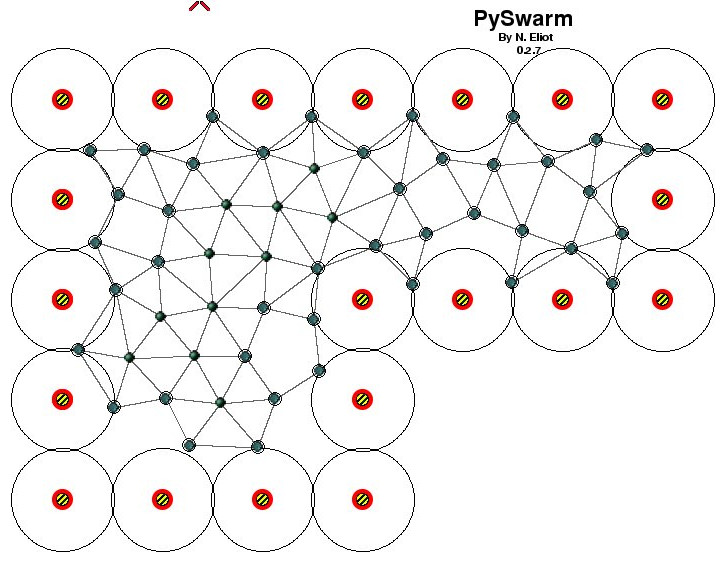
\includegraphics[width=5.5cm]{figures/REPEL52-3}
%% 	 \label{emerge:Repel52-3}
%% }
%% \subfigure[Stage 4]{
%% 	 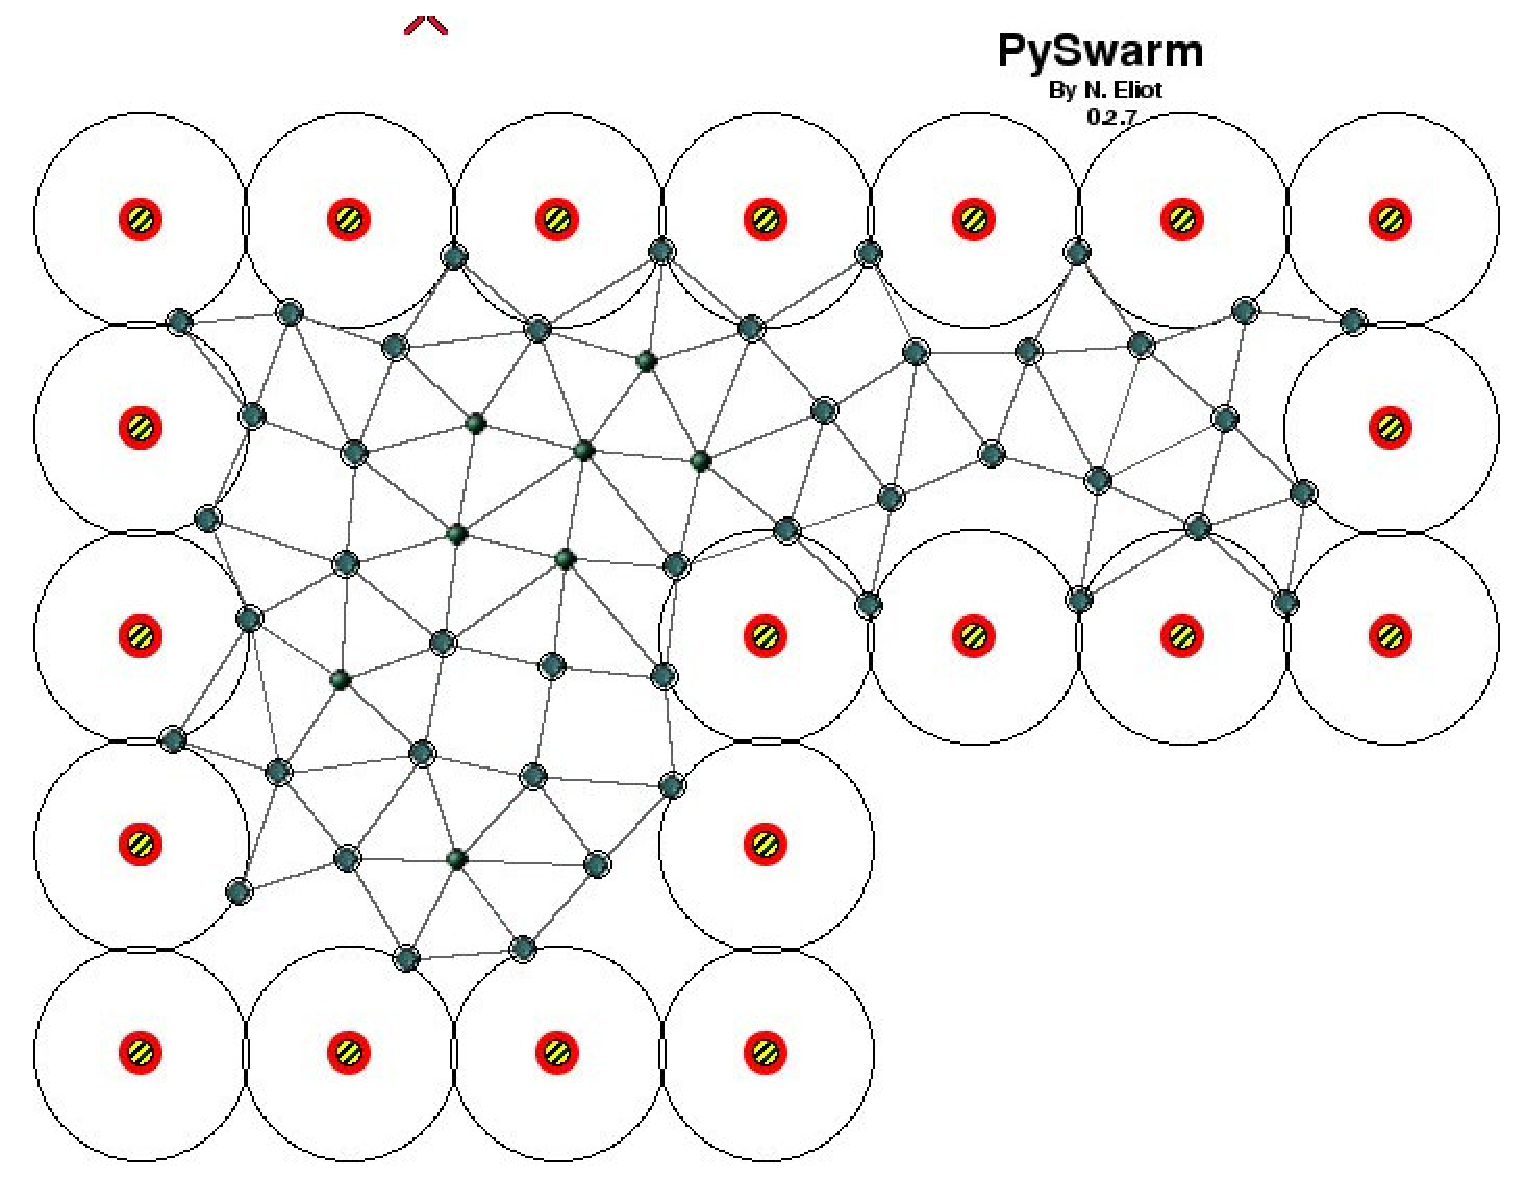
\includegraphics[width=5.5cm]{figures/REPEL52-4}
%% 	 \label{emerge:Repel52-4}
%% }
%% \subfigure[Stage 5]{
%% 	 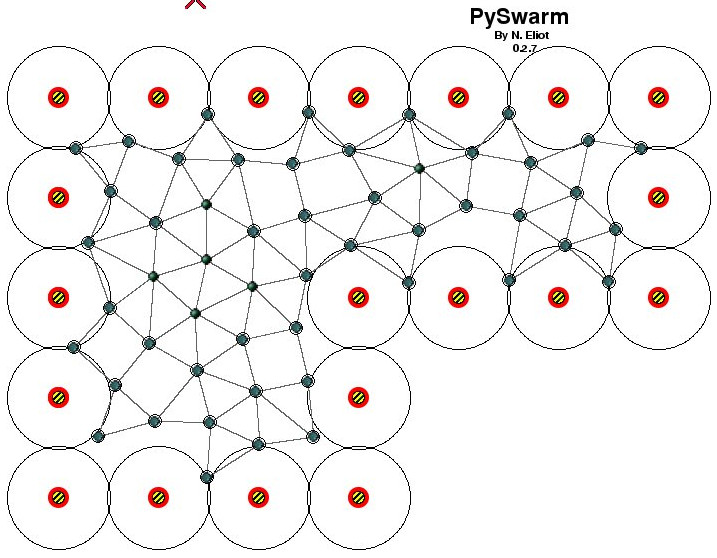
\includegraphics[width=5.5cm]{figures/REPEL52-5}
%% 	 \label{emerge:Repel52-5}
%% }
%% \subfigure[Stage 6]{
%% 	 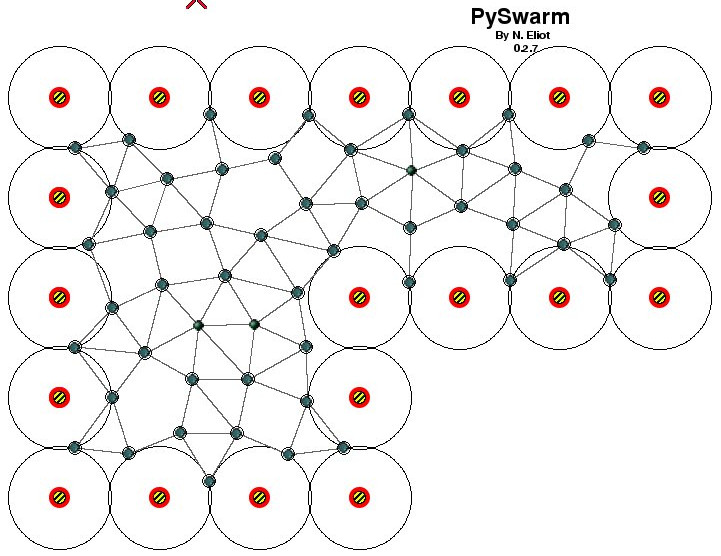
\includegraphics[width=5.5cm]{figures/REPEL52-6}
%% 	 \label{emerge:Repel52-6}
%% }
%% \subfigure[Stage 7]{
%% 	 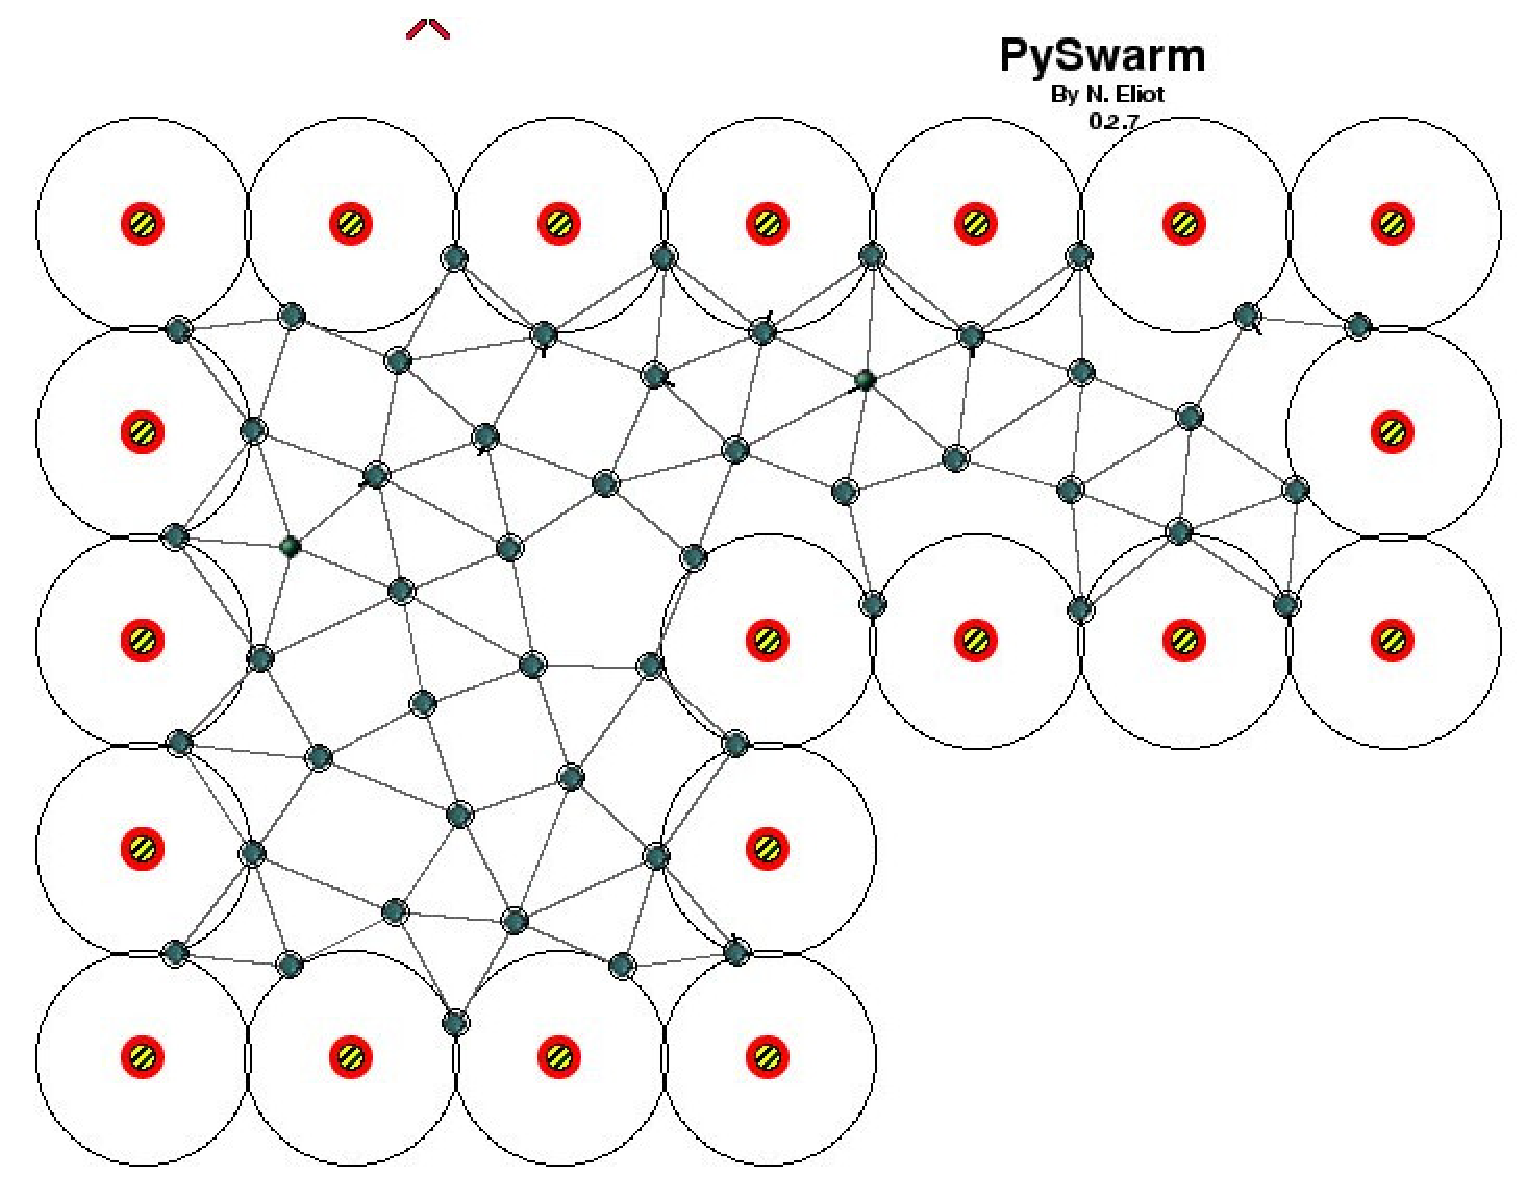
\includegraphics[width=5.5cm]{figures/REPEL52-7}
%% 	 \label{emerge:Repel52-7}
%% }
%% \subfigure[Stage 8]{
%% 	 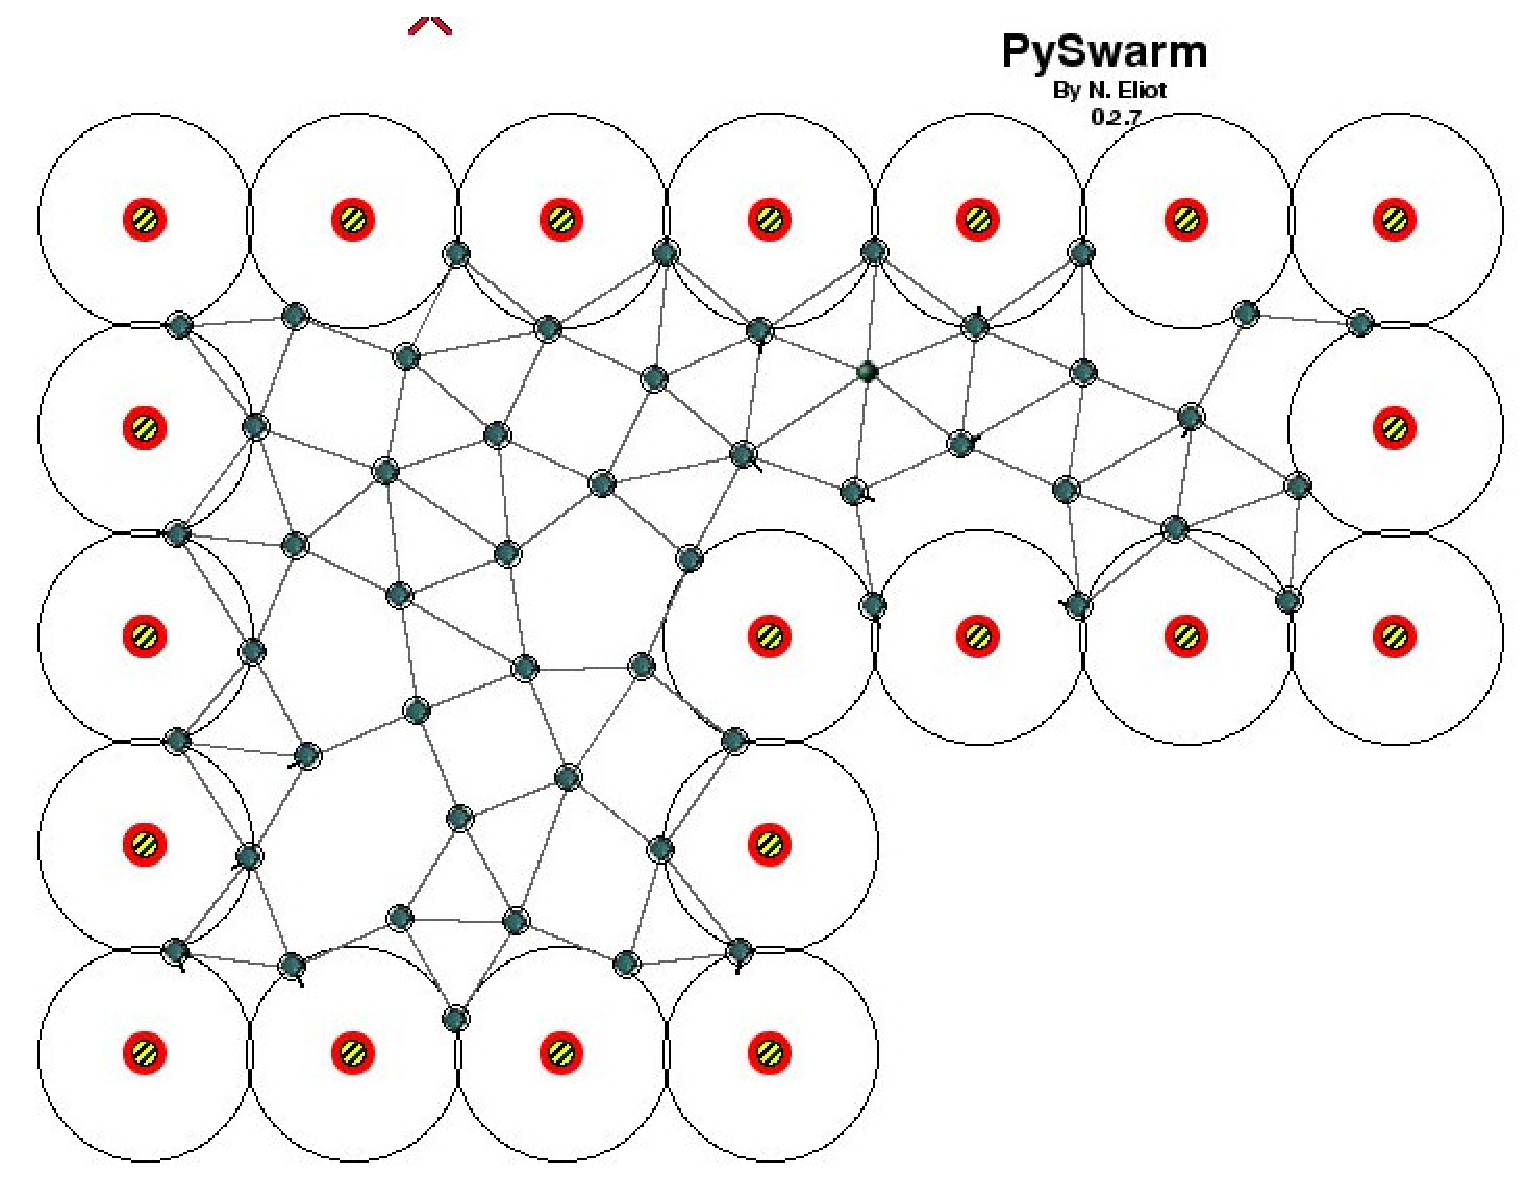
\includegraphics[width=5.5cm]{figures/REPEL52-8}
%% 	 \label{emerge:Repel52-8}
%% }
%% \caption{Space filling via repulsion}
%% \label{emerge:SwarmFloodRepel}
%% \end{figure}

\subsection{\textit{Inter-agent magnitude} analysis}
Figure~\ref{emerge:REPELFILL5055-MAG} shows the \textit{inter-agent vector magnitude} produced between the agents. The initial deployment of the swarm shows a large negative value due to the swarm being in a highly compressed state. This causes the swarm to expand rapidly. Following the initial expansion the agents enter a phase of very close adjustment as their positions move towards a maximum expansion point. Eventually the agents are distributed to their maximum positions with the \textit{inter-agent vector magnitude} stabilises to zero with no variation. At this stage the swarm has stopped moving. This effect cannot be detected by using the distance metric which will simply show a distribution distance with a fixed variance. Having a fixed variance does not indicate the agents have stopped moving as agents could be moving in sympathy to each other creating a net change of zero.

\begin{figure}
\begin{center}
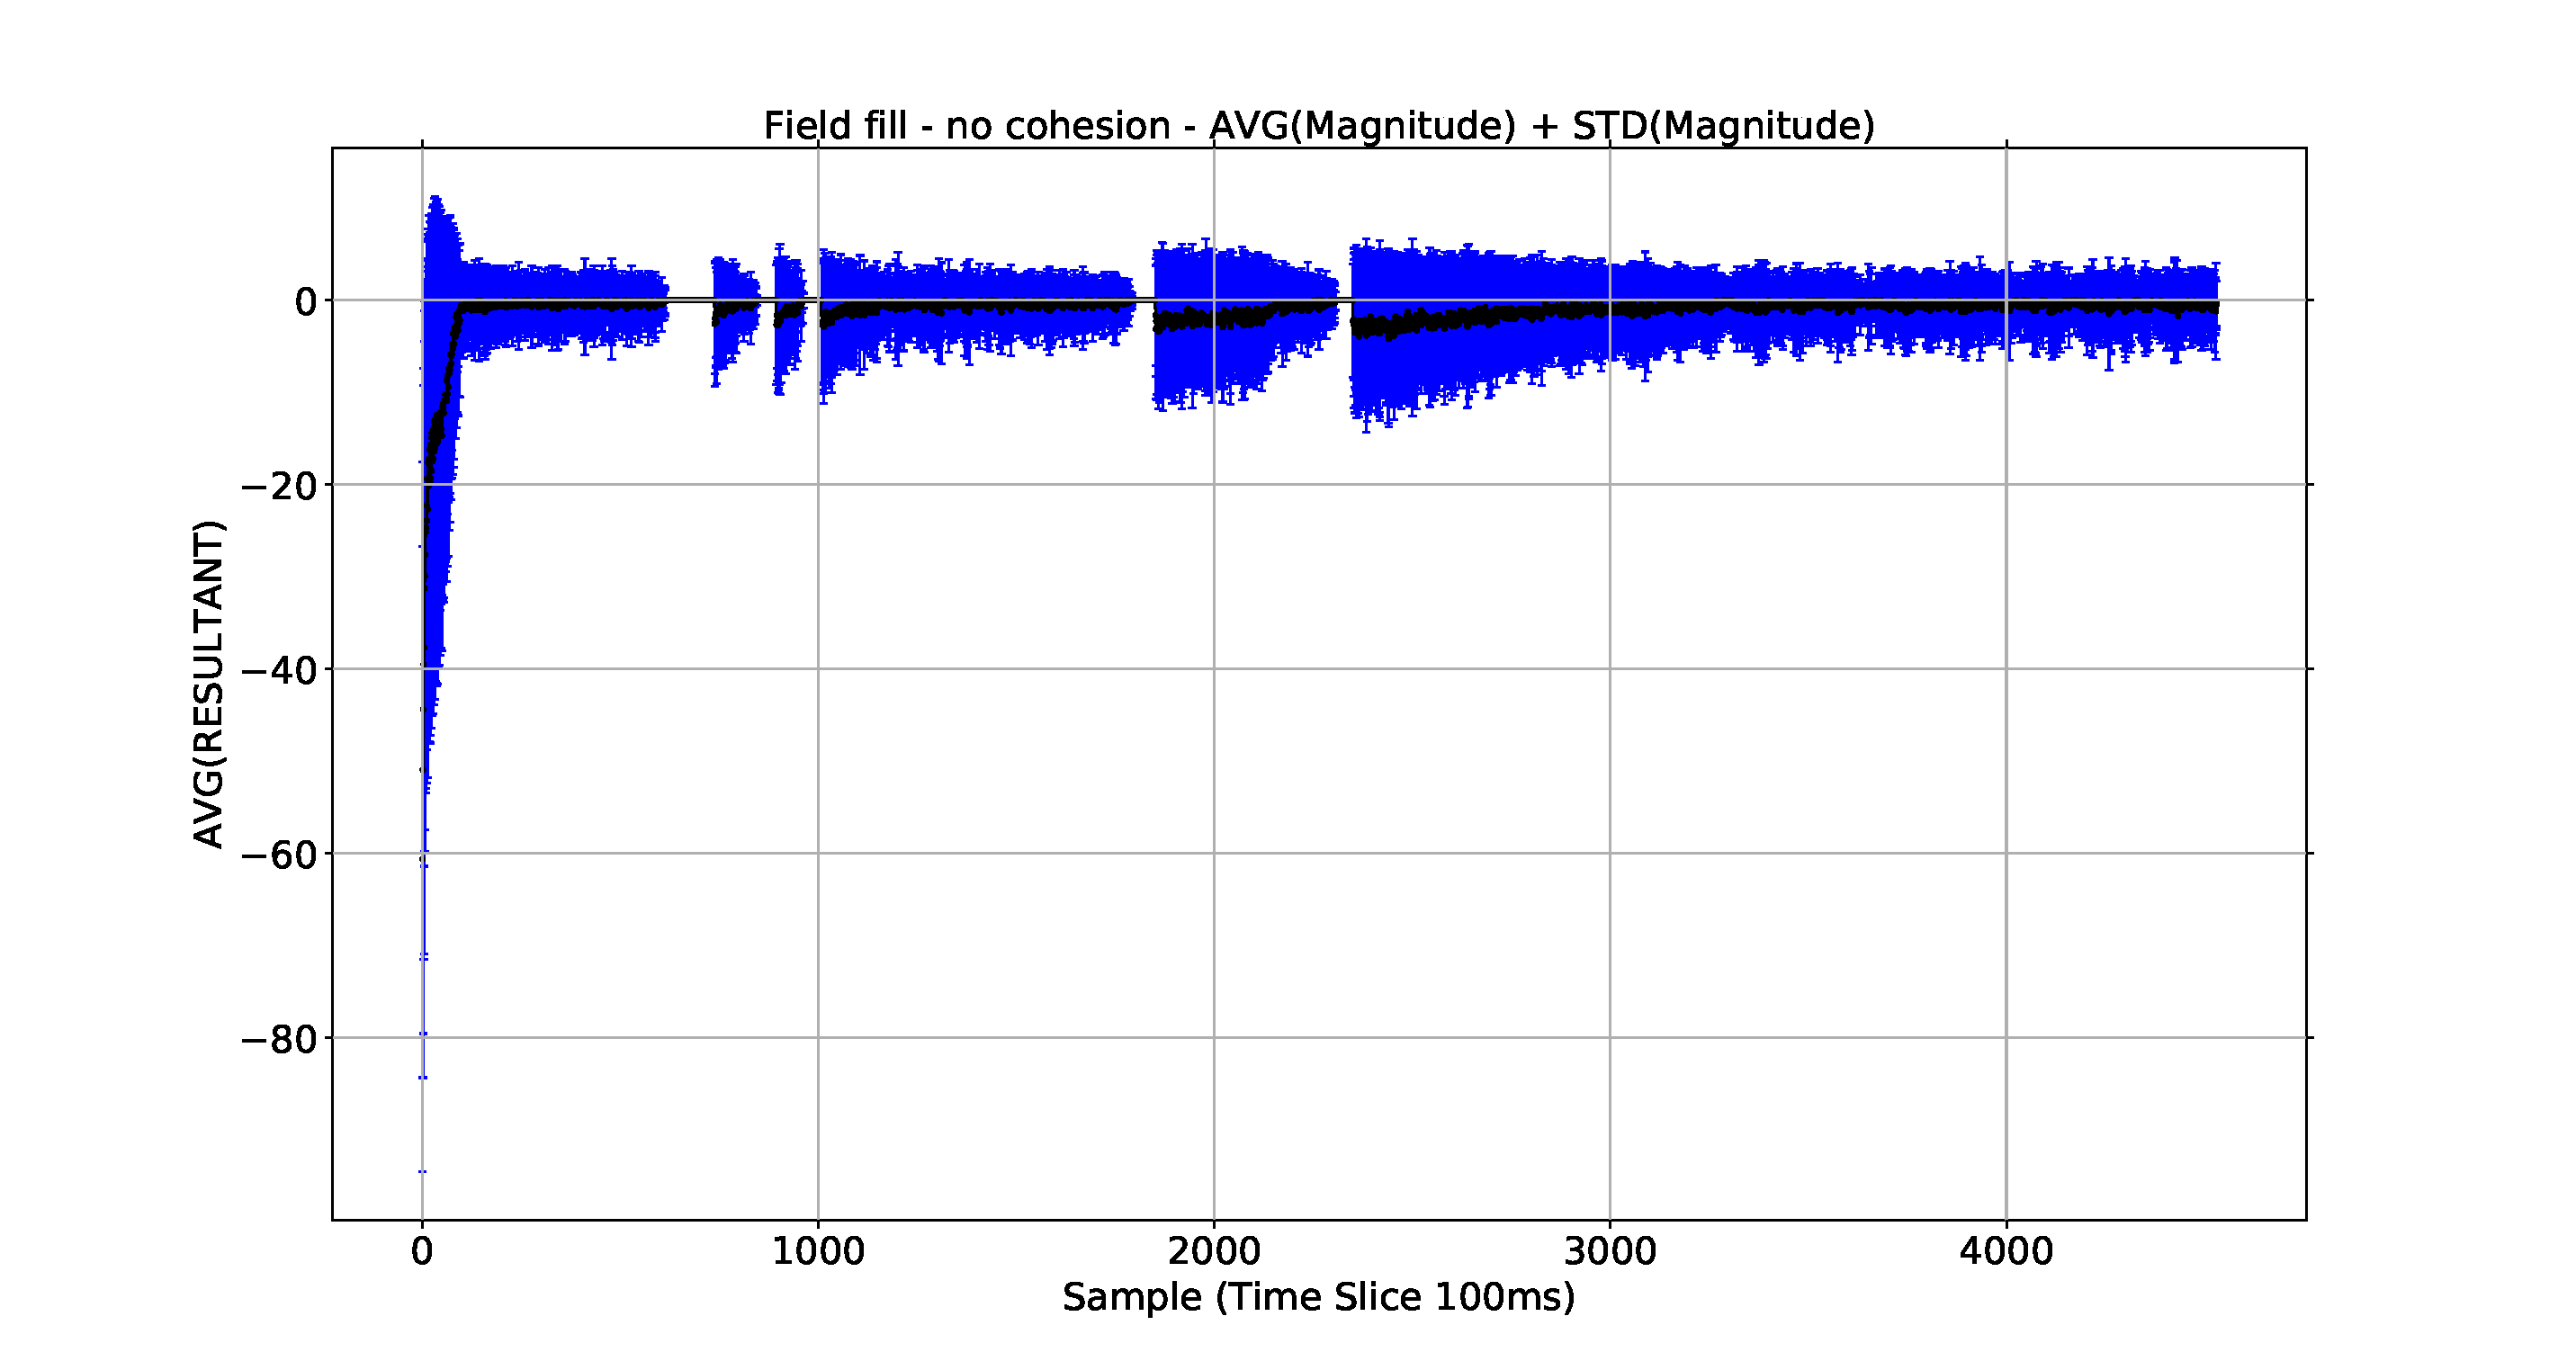
\includegraphics[width=8.5cm]{figures/REPELFILL5055-MAG}
\end{center}
\caption{Magnitude metric 0-450 seconds\label{emerge:REPELFILL5055-MAG}}
\end{figure}

Figure~\ref{emerge:REPELFILL5055-MAG-1-2} shows the initial settling period of the swarm in greater detail between 0 and 65 seconds. The graph shows that the settling period lasts for approximately 55 seconds following the initial expansion of the swarm from 0 to 10 seconds. The initial deployment of swarm has a highly negative \textit{interaction vector magnitude} causing rapid expansion. From 10 second until approx 62 seconds the agents \textit{inter-agent vectors} cause the agents to spread within the space. When the agents reach the limits of the repulsion field effect they stop moving. The \textit{inter-agent vector magnitude} stabalises to zero and all the agents stop moving.

\begin{figure}
\begin{center}
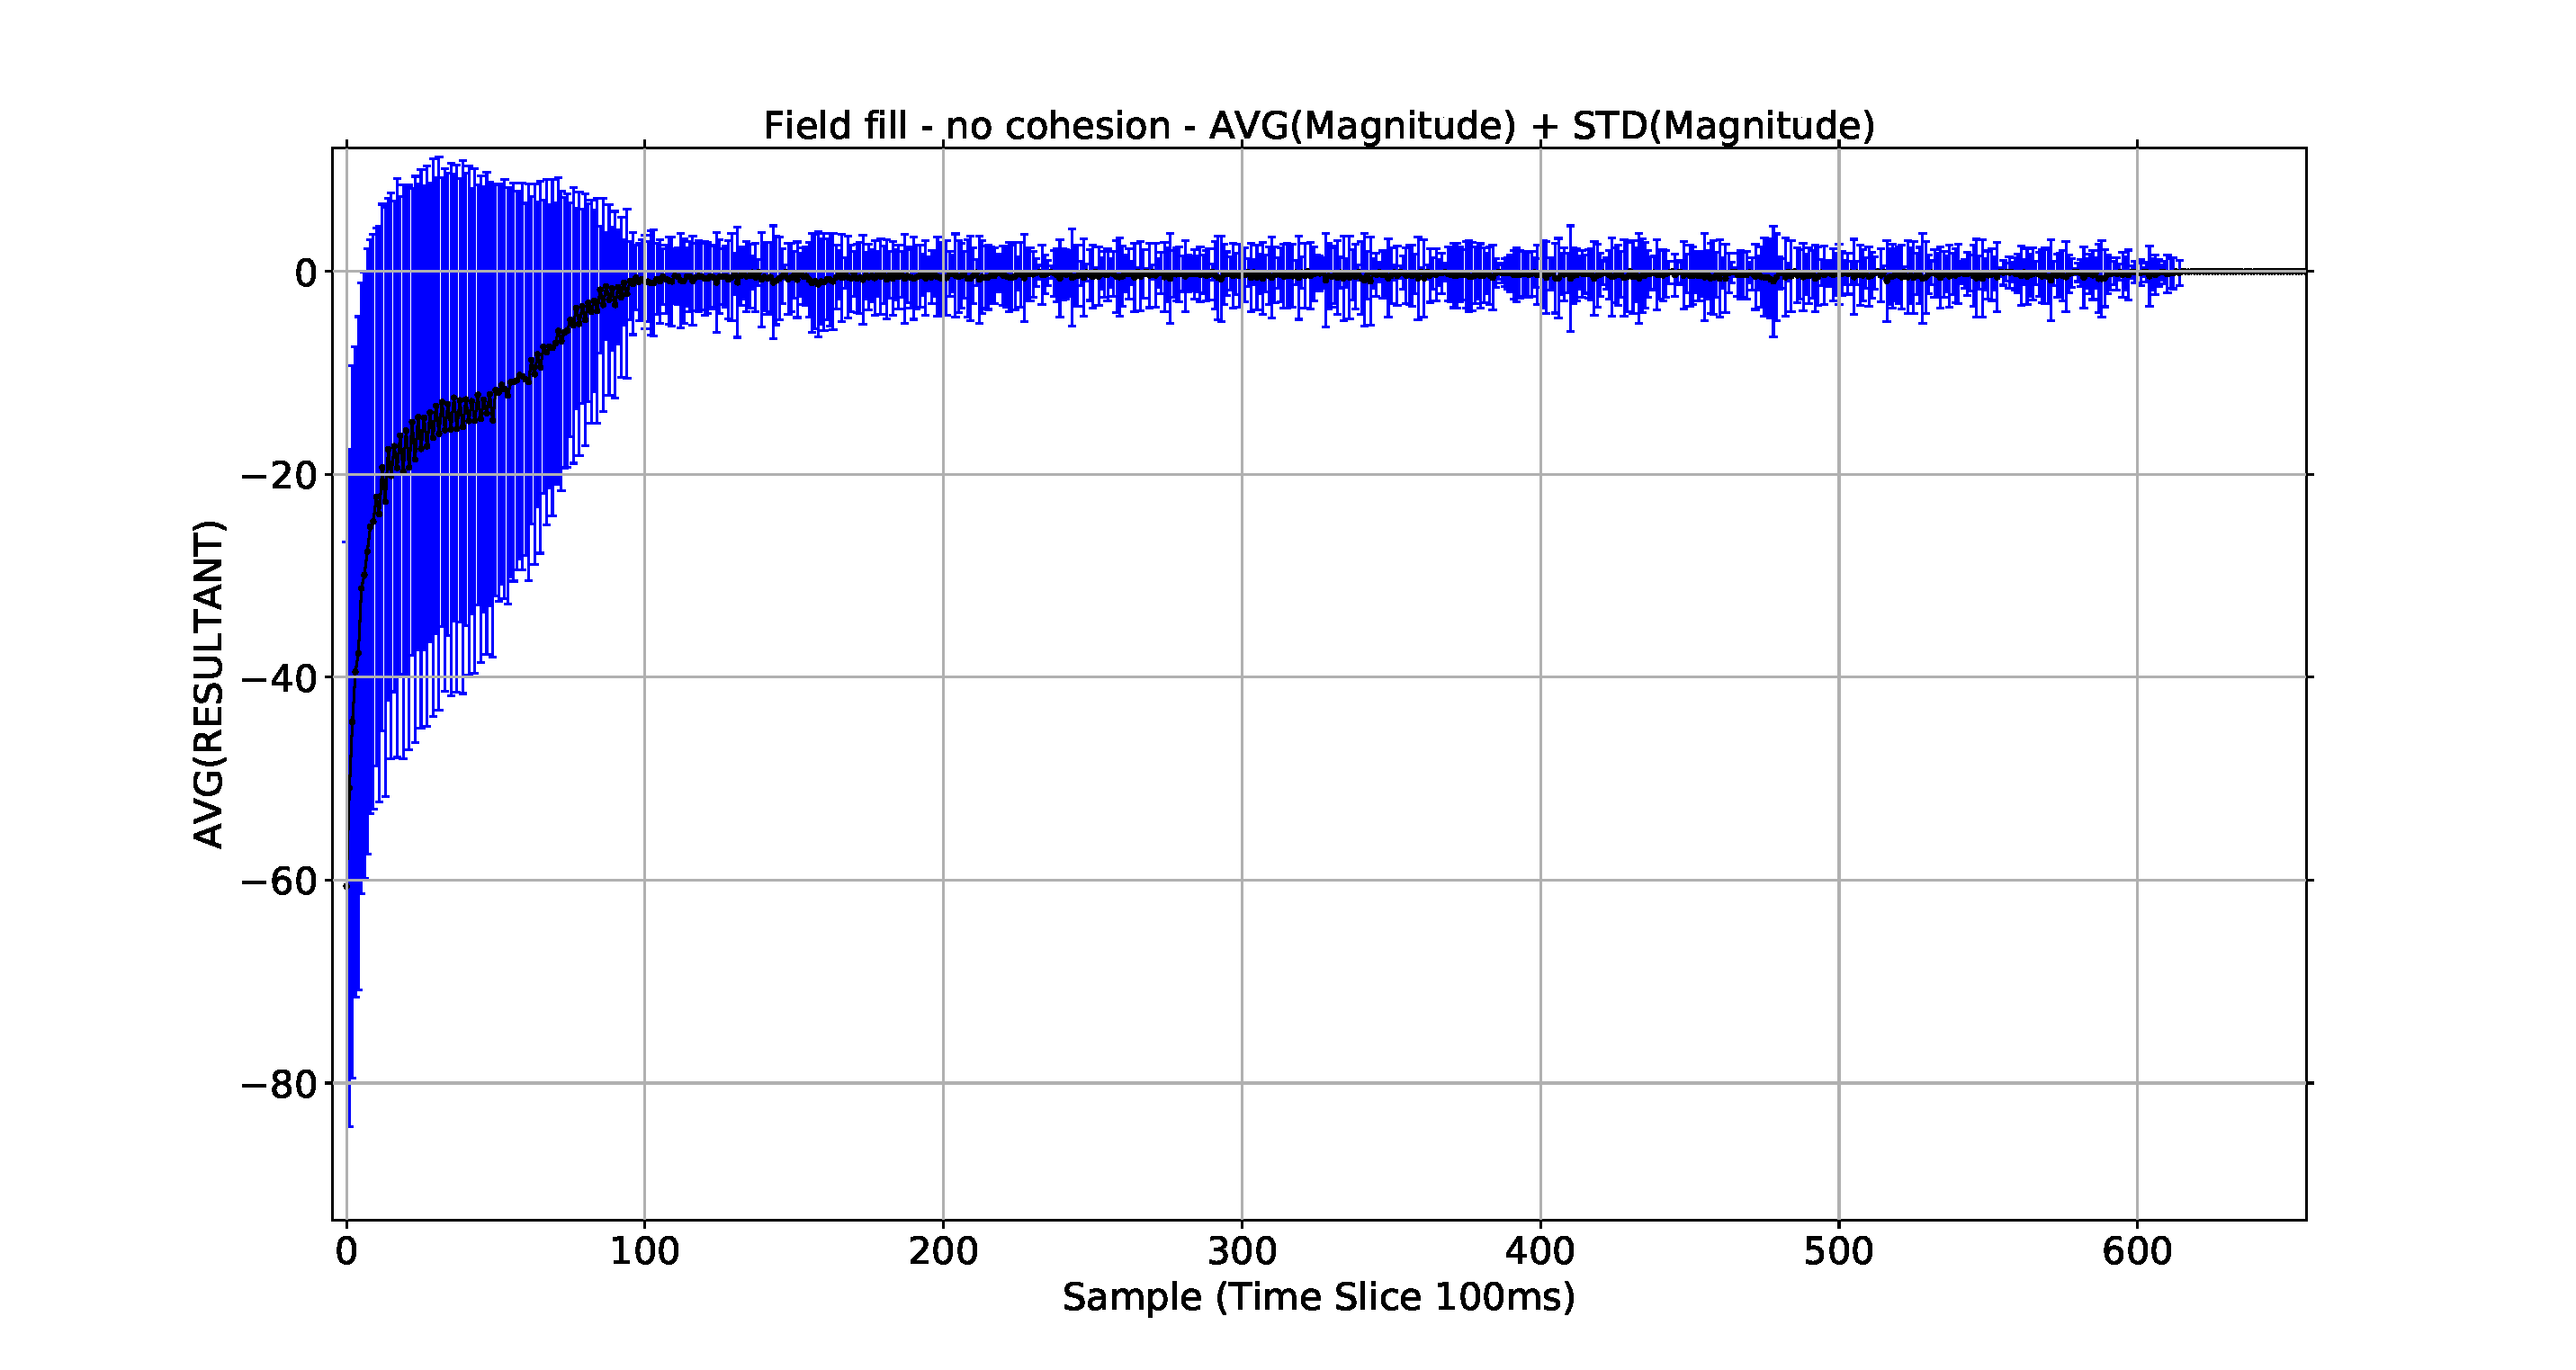
\includegraphics[width=8.5cm]{figures/REPELFILL5055-MAG-1-2}
\end{center}
\caption{Magnitude metric 0-65 seconds\label{emerge:REPELFILL5055-MAG-1-2}}
\end{figure}

Figure~\ref{emerge:REPELFILL5055-MAG-2-3} shows a detailed view of the magnitude for the swarm at the first repulsion field increment at approximately 73.5 seconds. The repulsion field effect is incremented by 1 unit. The field effect change is sufficient to allow agents to be within the neighbour field effect range. The agents are already distributed from the initial expansion so there is a `trickling' movement that occurs as the agents increase the area of the swarm within the space. The area containment is not causing any distrurbance to the swarm at this stage so the swarm settles to zero (84.5 seconds). As with the initial expansion all the agents are distributed such that they are on or beyond the limits of the repulsion field effect and the swarm stops moving. This process of incrementing the field effect and the swarm stablising continues until the field effect causes the swarm to expand to a point that it fills the area and the agents are unable to move sufficiently to stop interacting.

\begin{figure}
\begin{center}
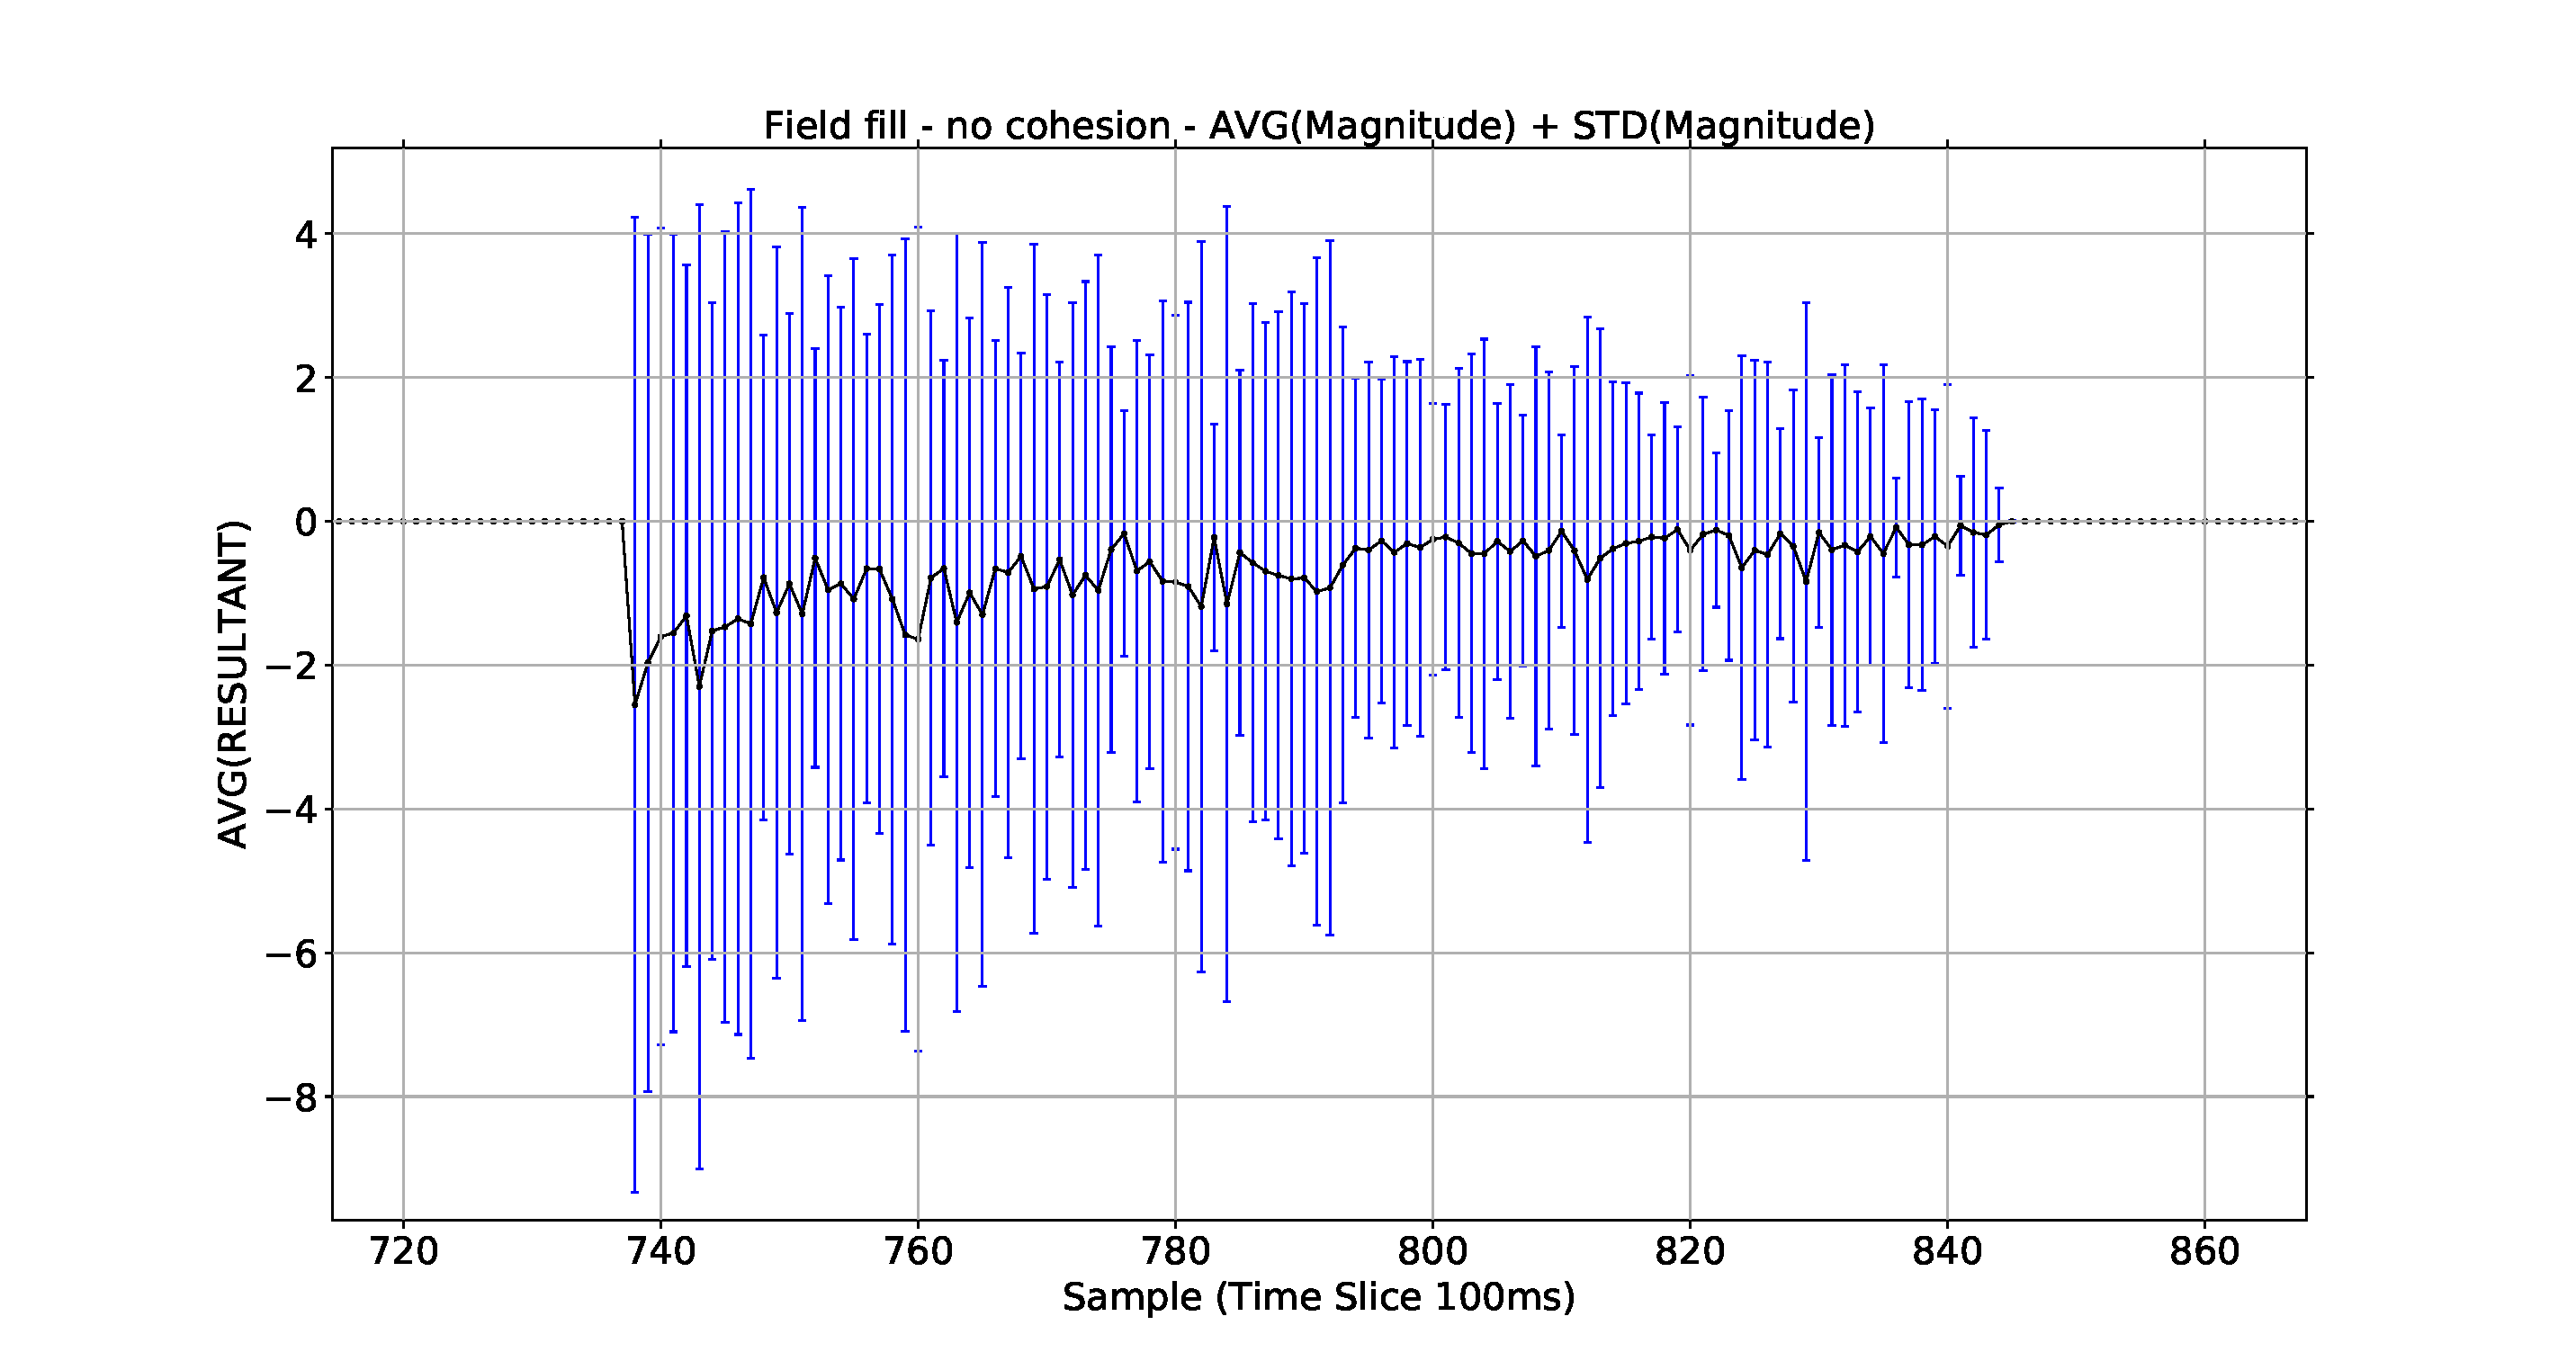
\includegraphics[width=8.5cm]{figures/REPELFILL5055-MAG-2-3}
\end{center}
\caption{Magnitude metric 70-85 seconds\label{emerge:REPELFILL5055-MAG-2-3}}
\end{figure}

Figure~\ref{emerge:REPELFILL5055-MAG-8} shows the final part of the simulation where the swarm's resultant magnitude is unable to stablise completely. The graph shows the increment at approximately 230 seconds creating swarm movement which slowly increasing towards zero as the swrm expands however the \textit{inter-agent vector magnitude} is not able to reach zero. The swarm's agents are bound by the space cannot distribute themselves to a point where the field effect overlap is overcome. The \textit{inter-agent vector magnitude} average remains below 0 indicating there is a `pressure' that cannot be overcome and the agents are in continuous movement. At this stage it is possible for all the agents to obtain a state of equilibrium and for the average magnitude to stablise but owing to their containment the average magnitude would not be able to rise to zero. The swarm has therefore expanded to fill the space.

\begin{figure}
\begin{center}
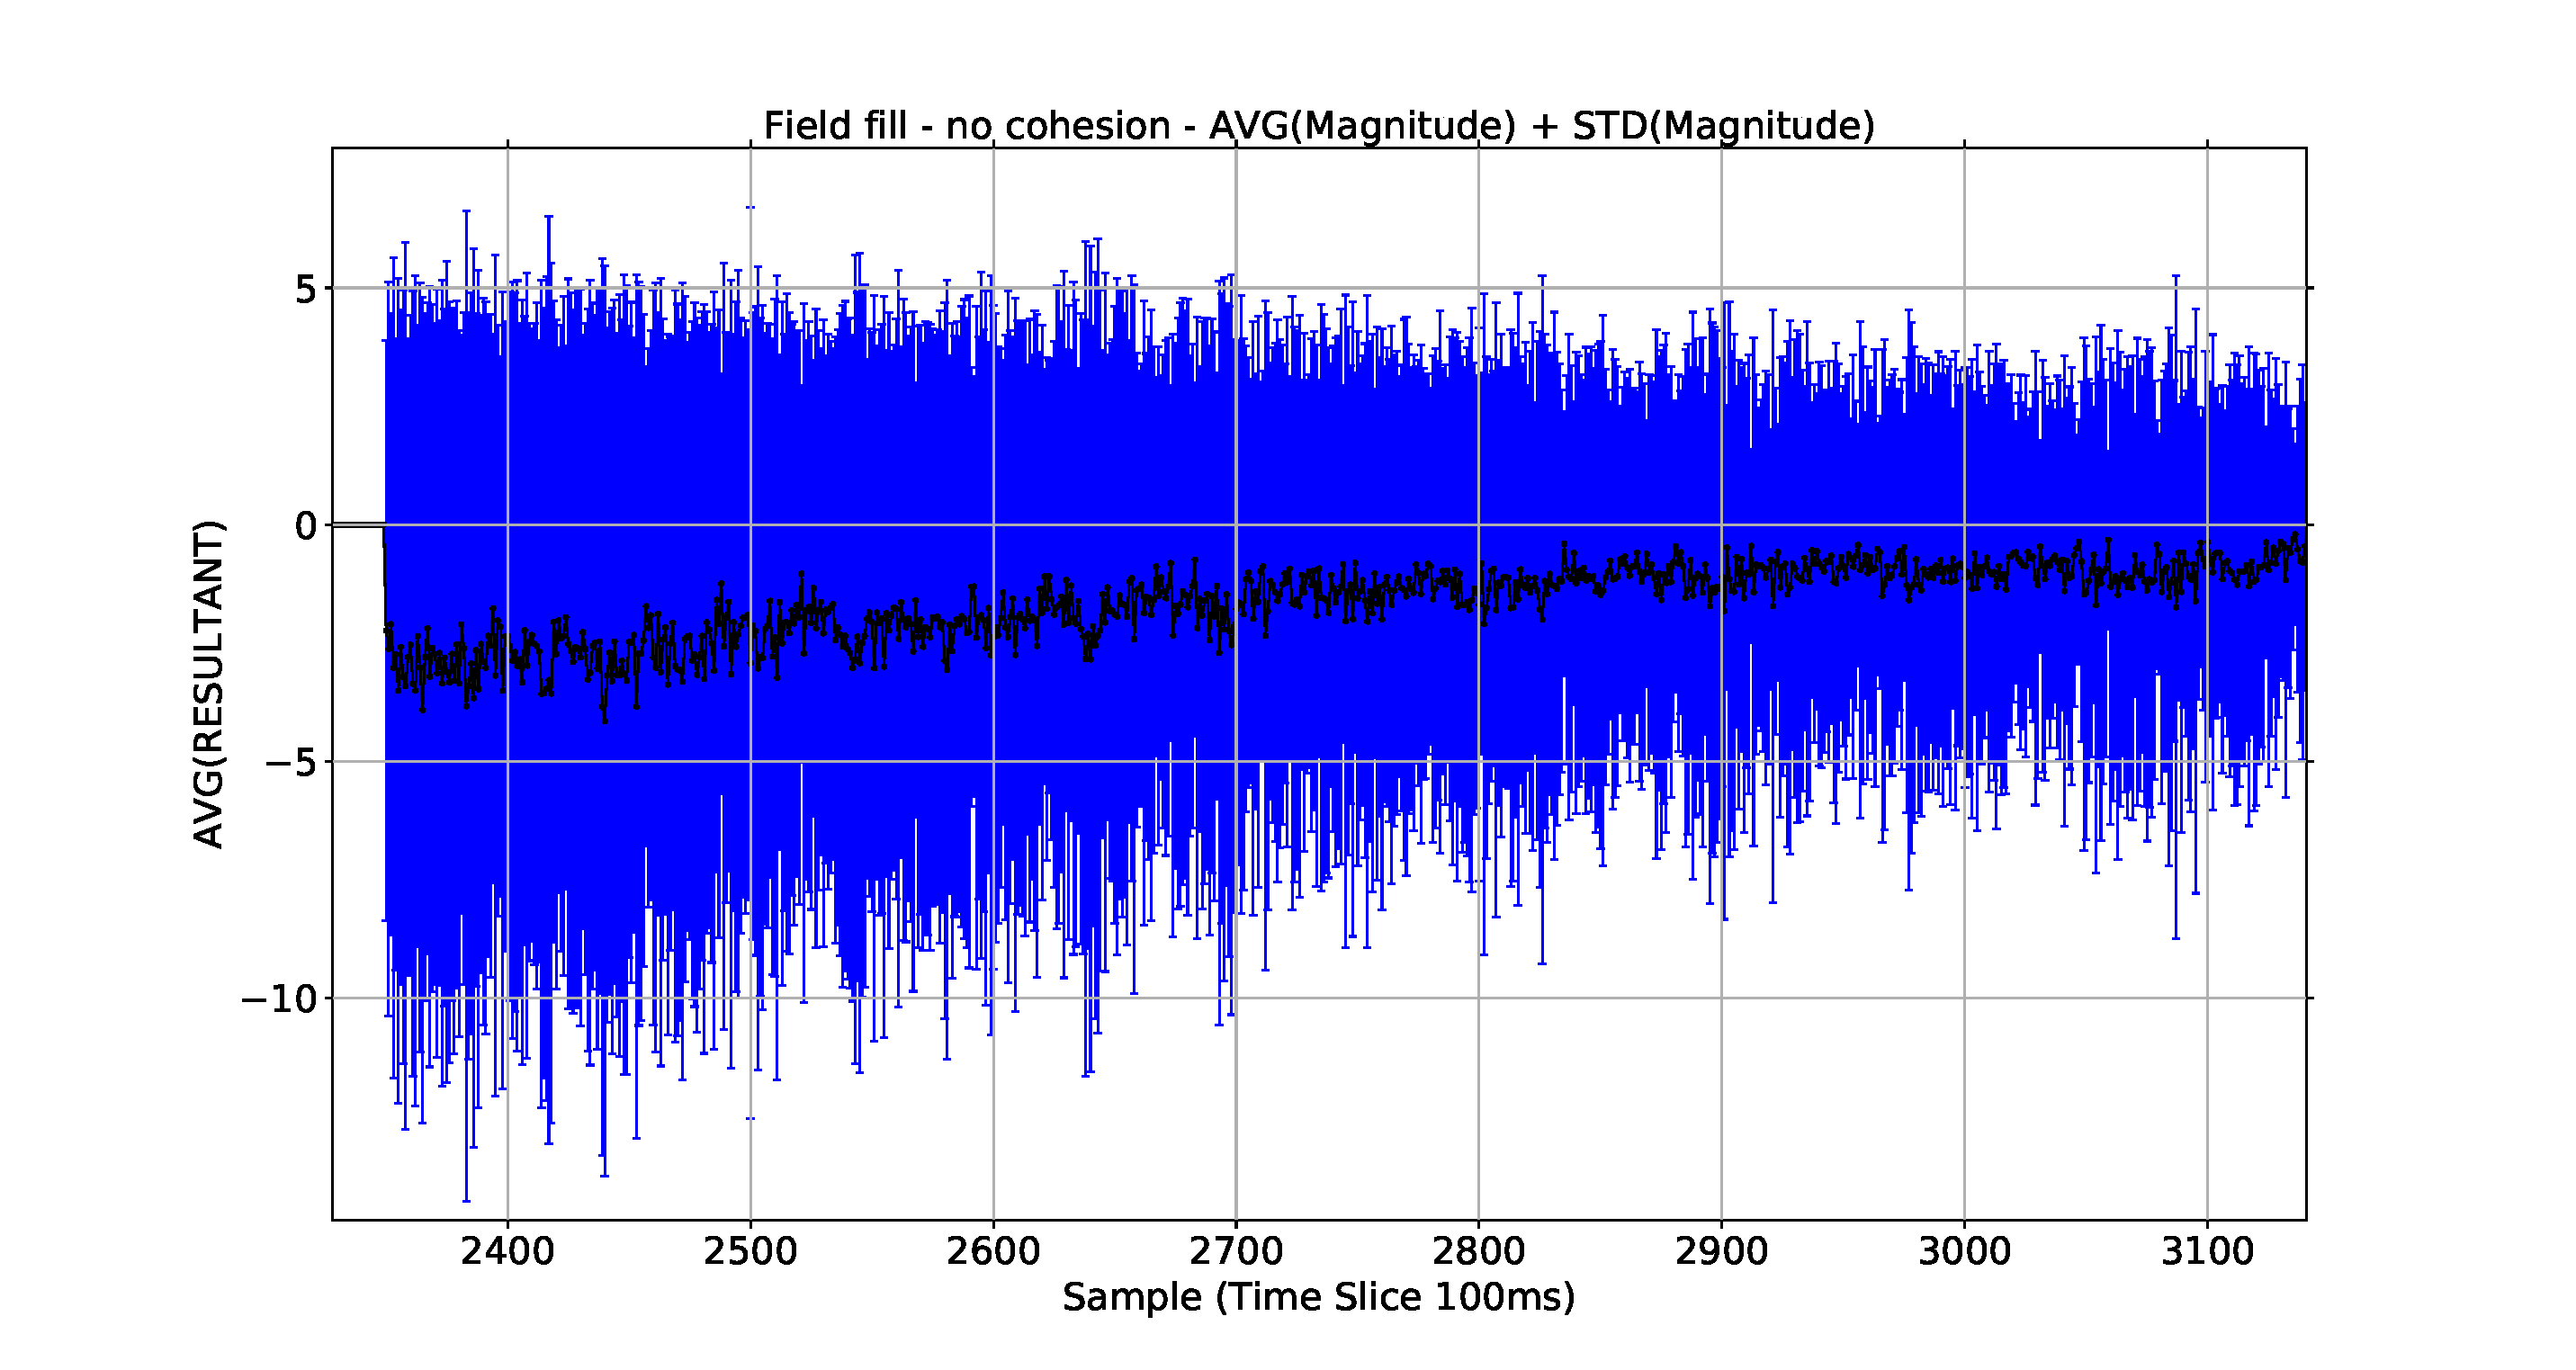
\includegraphics[width=8.5cm]{figures/REPELFILL5055-MAG-8}
\end{center}
\caption{Magnitude metric 235-315 seconds\label{emerge:REPELFILL5055-MAG-8}}
\end{figure}

\subsection{Distance analysis}
Figure~\ref{emerge:REPELFILL5055-DIST} shows the distance metric for the same simulation as above. The initial deployment shows the agents are quite close together but immediately expand, the variance reduces as the agents become more evenly distributed. 

\begin{figure}
\begin{center}
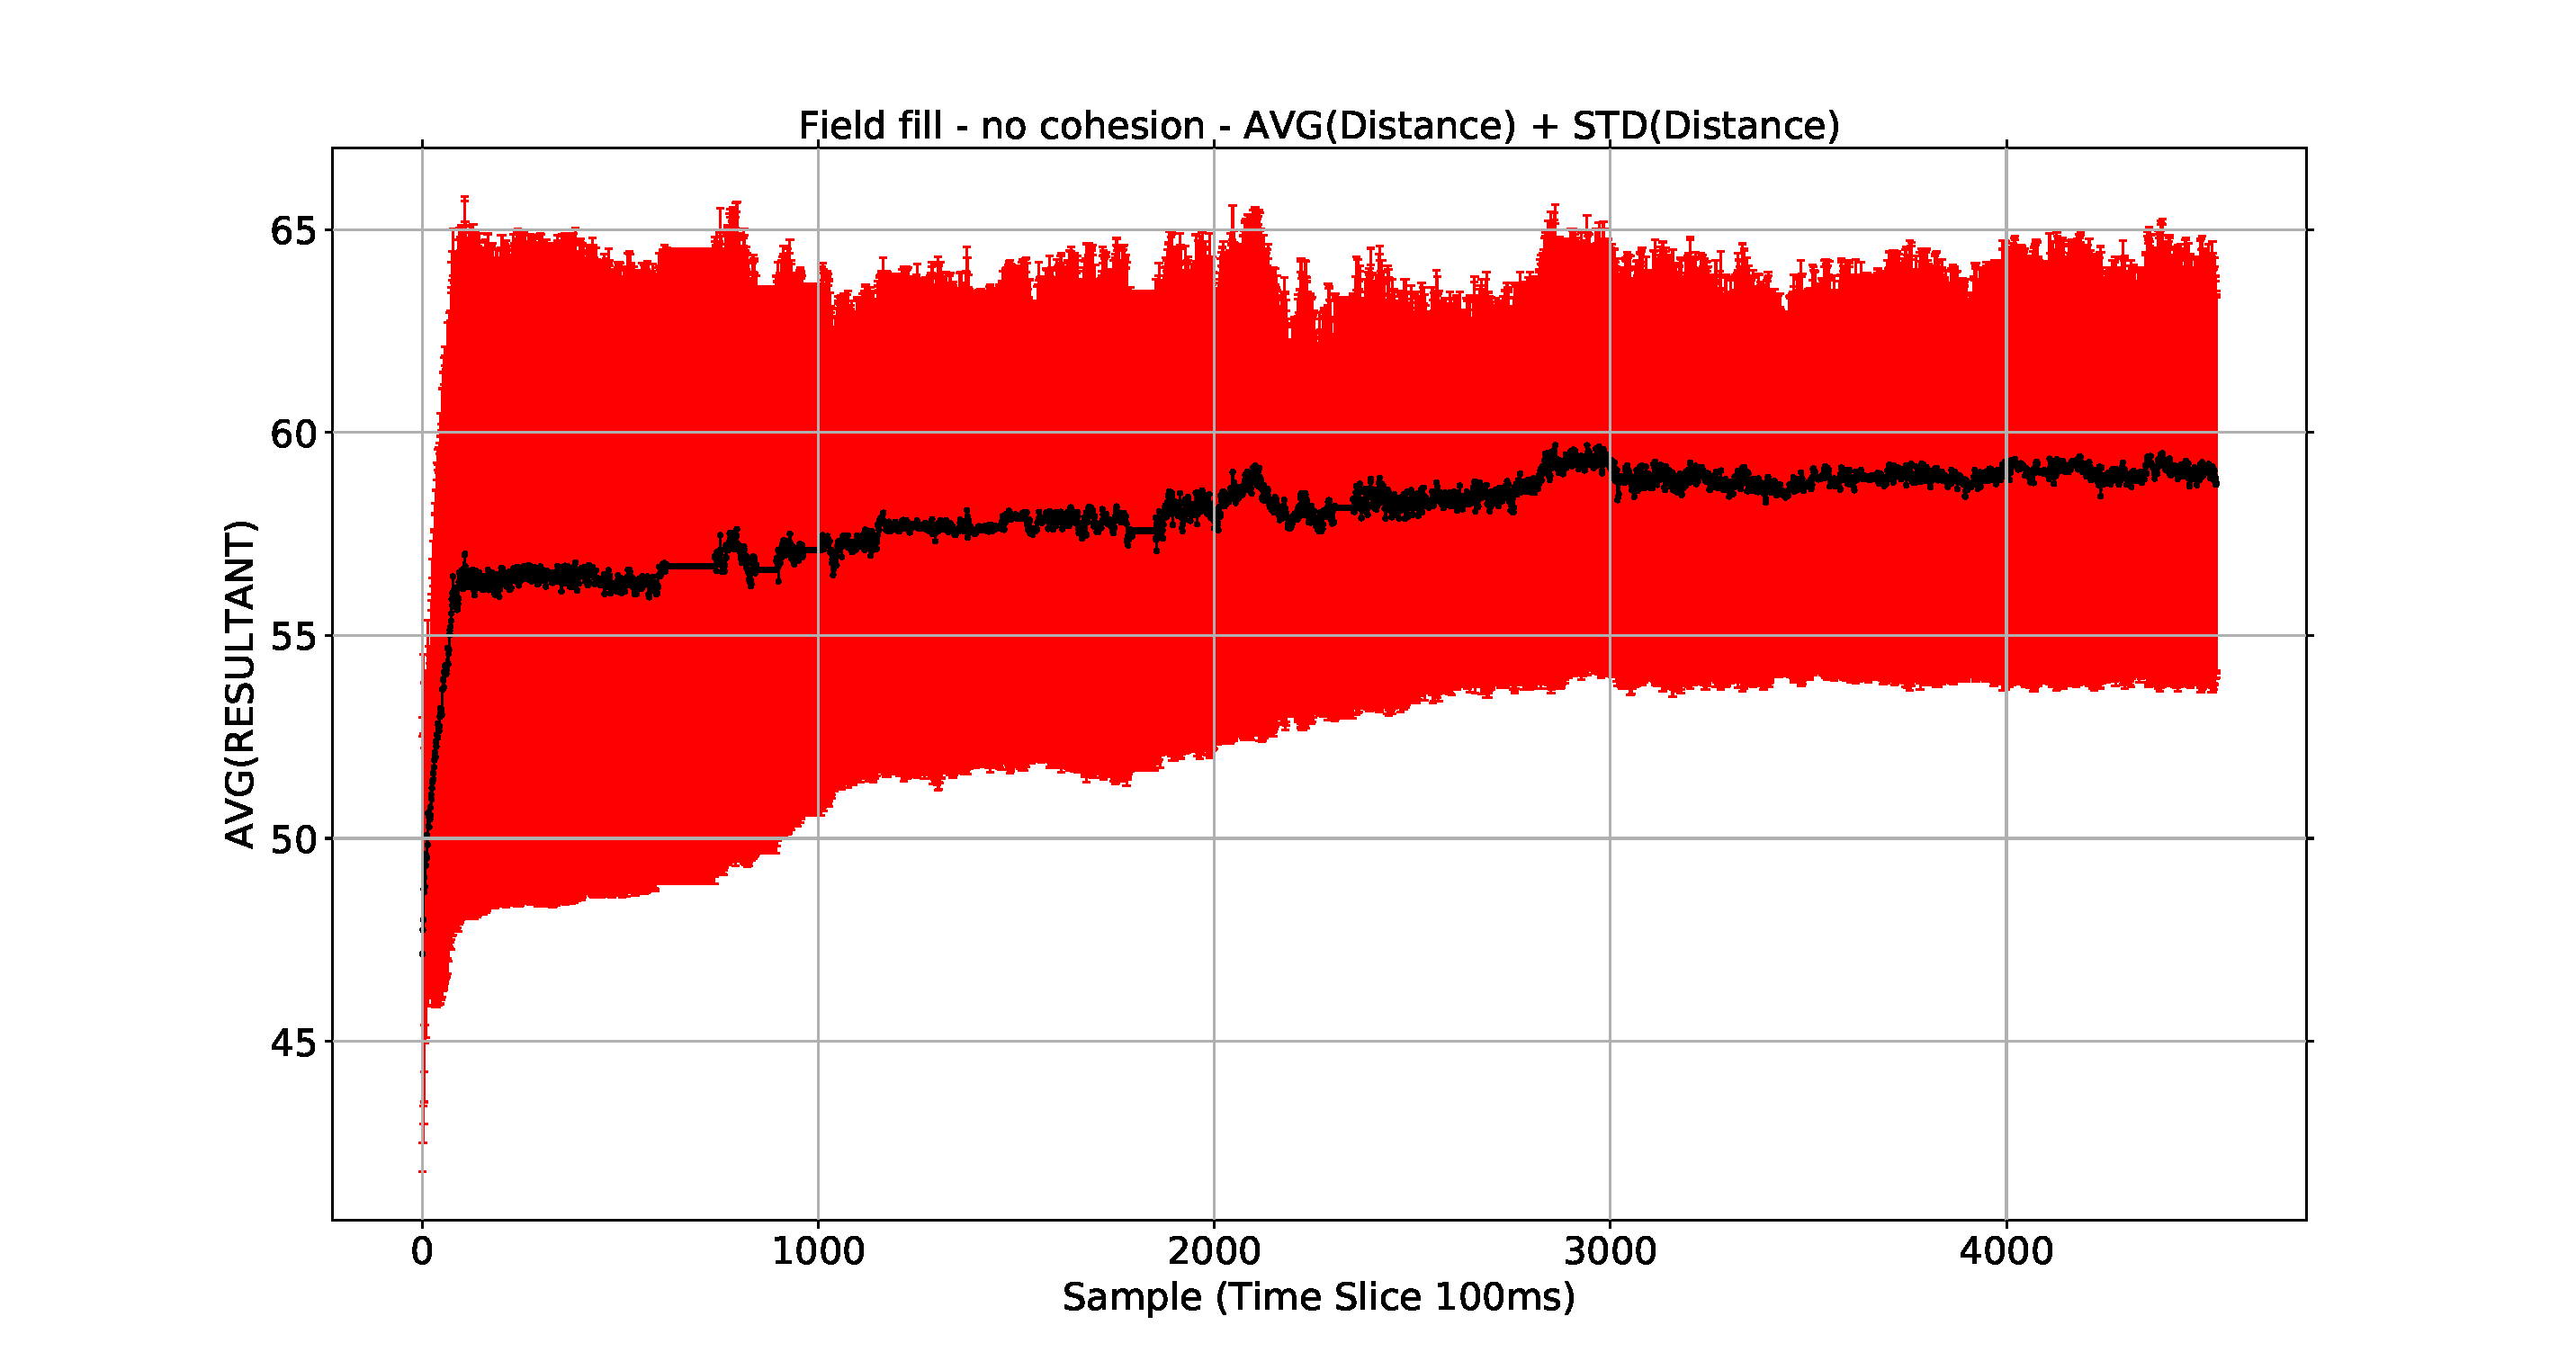
\includegraphics[width=8.5cm]{figures/REPELFILL5055-DIST}
\end{center}
\caption{Distance metric 0-450 seconds\label{emerge:REPELFILL5055-DIST}}
\end{figure}

Figure~\ref{emerge:REPELFILL5055-DIST-1} shows the period when the swarm has initially expanded to a point that the distances appear to stabilise. The stable state is shown as a constant average distance with a constant variance. It cannot be assumed that the agents have stopped moving at this point in the simulation. Agents could change positions such that the average variance is unaffected although this is unlikely. Over this same period the magnitude is zero as shown in~Figure~\ref{emerge:REPELFILL5055-MAG}. These two facts therefore allow the swarms state to be fully realised. The agents are distributed unevenly and are static.

\begin{figure}
\begin{center}
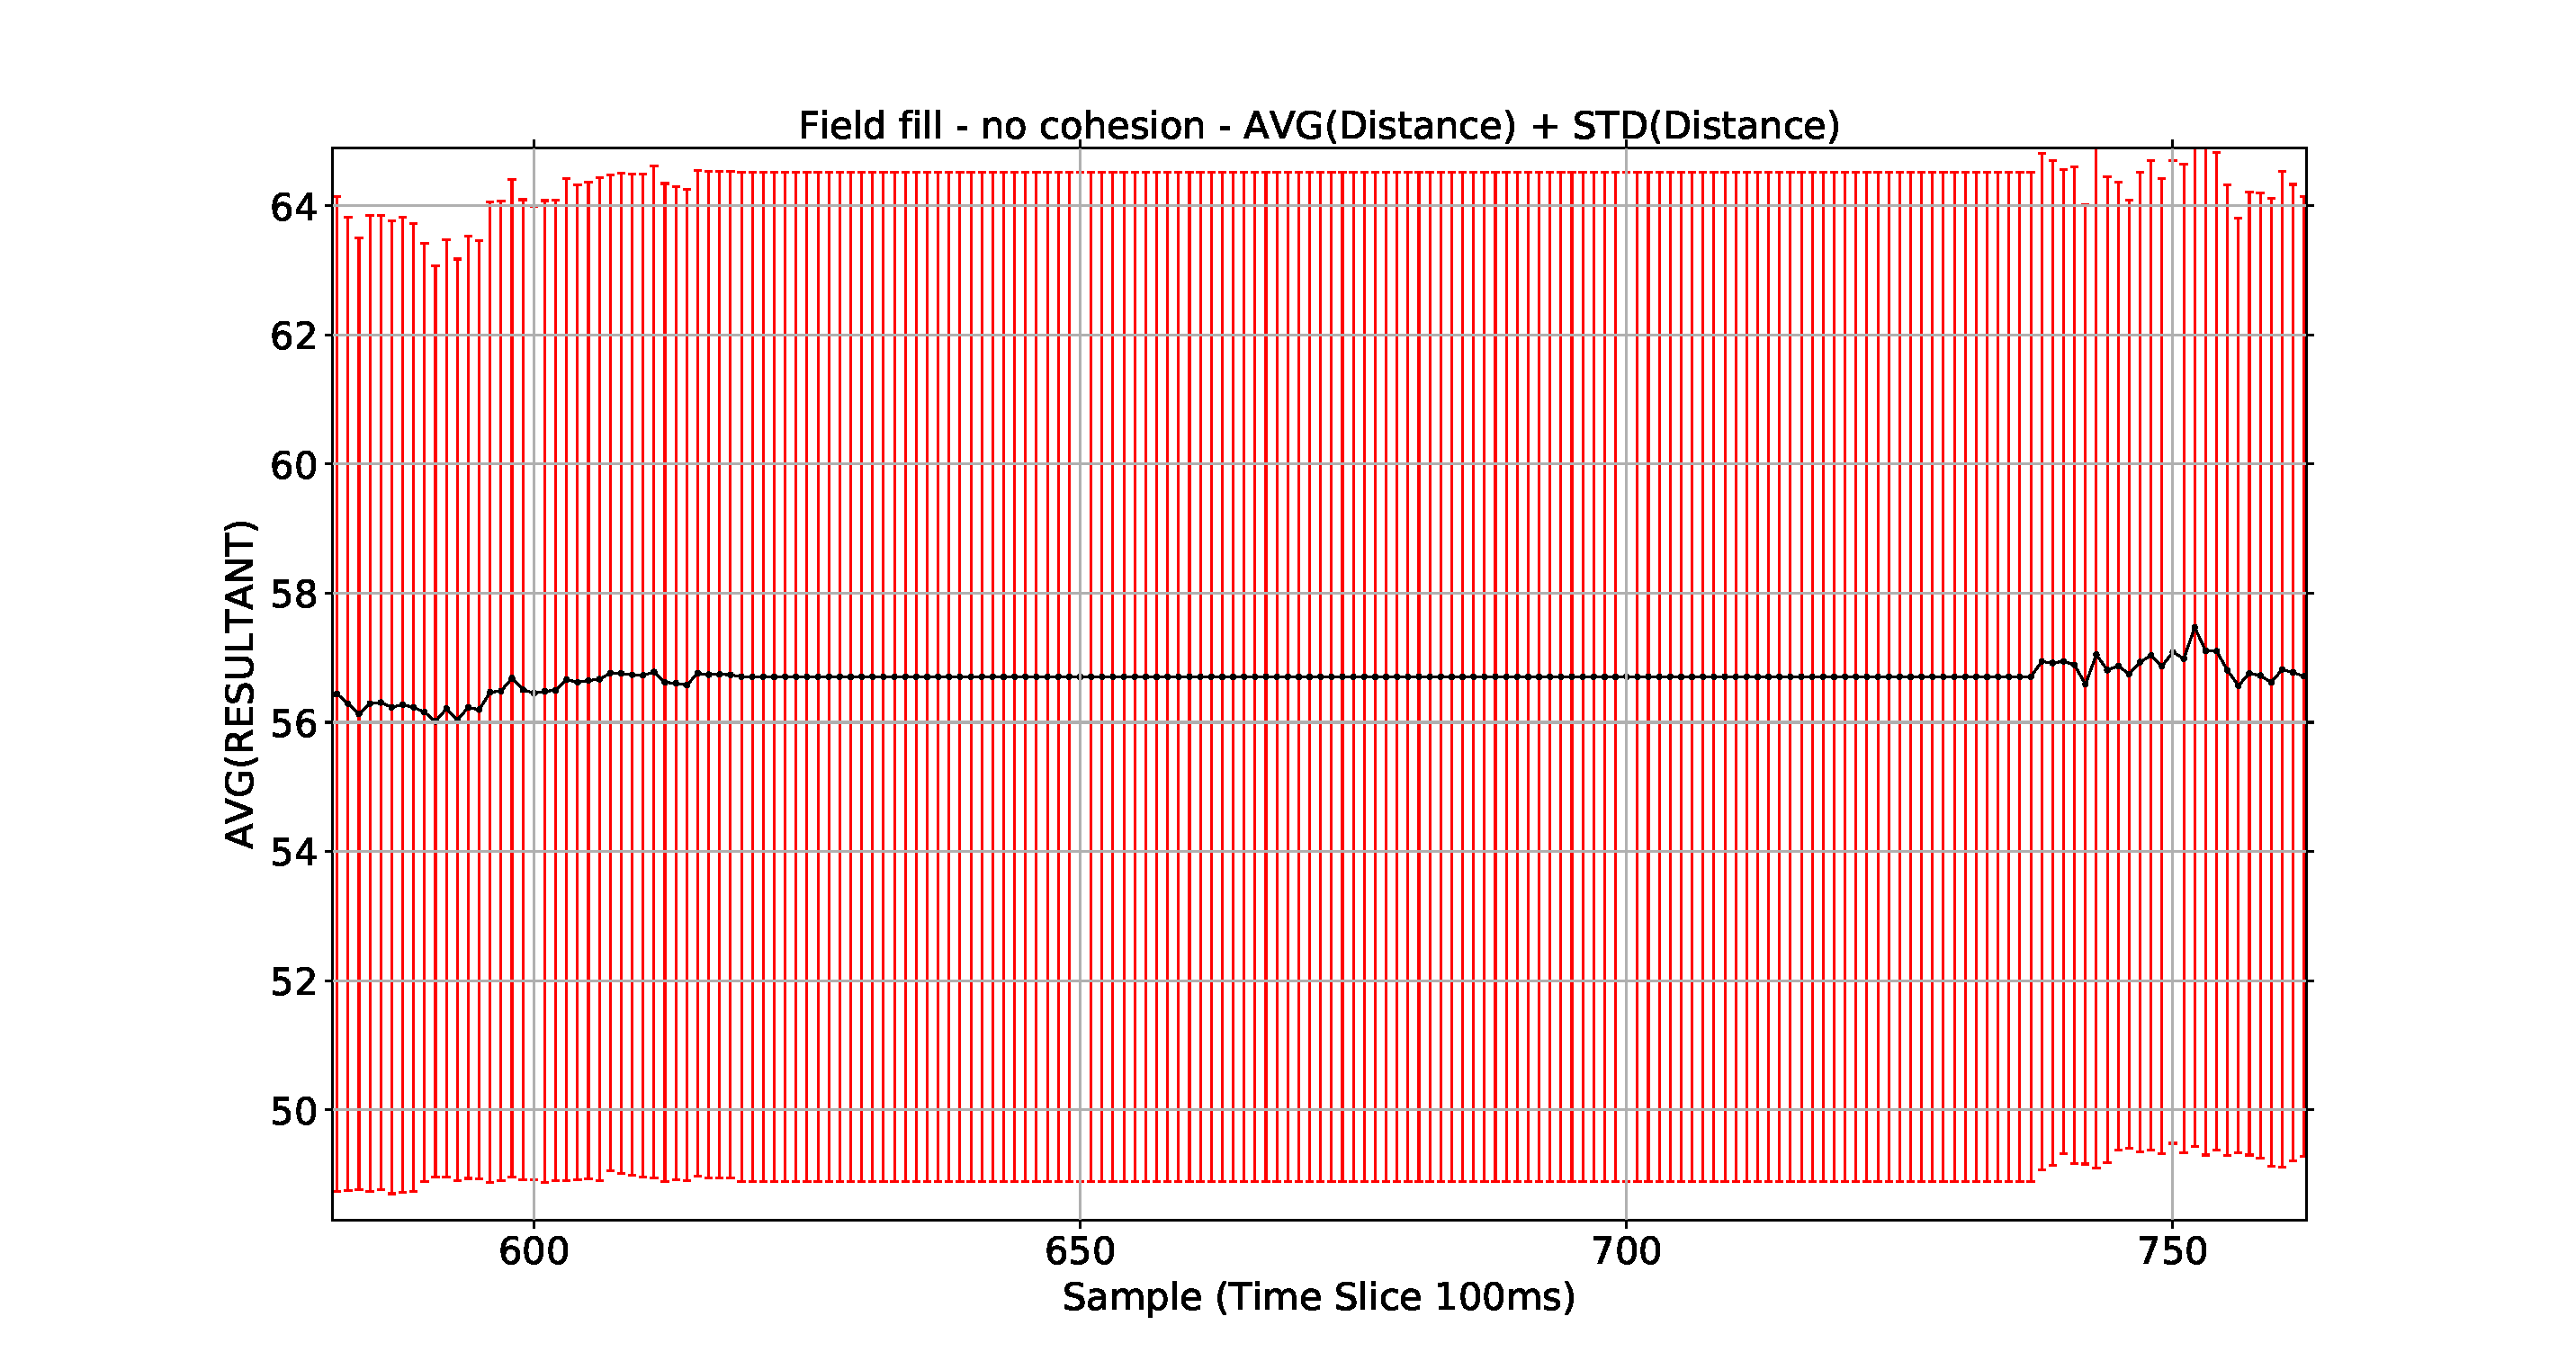
\includegraphics[width=8.5cm]{figures/REPELFILL5055-DIST-1}
\end{center}
\caption{Distance metric 60-75 seconds\label{emerge:REPELFILL5055-DIST-1}}
\end{figure}

Figure~\ref{emerge:REPELFILL5055-DIST-1-2} shows the effect of the first increment of the repulsion field effect increment (50-51 units). The swarm agents move to equalise the \textit{inter-agent vectors} by increasing the distance between the agents. The average distance changes very little due to the irregular distribution of the agents (there is no cohesion to help balance the distribution). The variance in the distance has reduced as the agents are more evenly distributed. At this stage the agents are not filling the space (\textit{inter-agent vector magnitude} has resolved to 0)~(Figure~\ref{emerge:REPELFILL5055-MAG-2-3}). The two metrics together indicate that the swarm's agent distribution is more even but the swarm is not filling the space.

\begin{figure}
\begin{center}
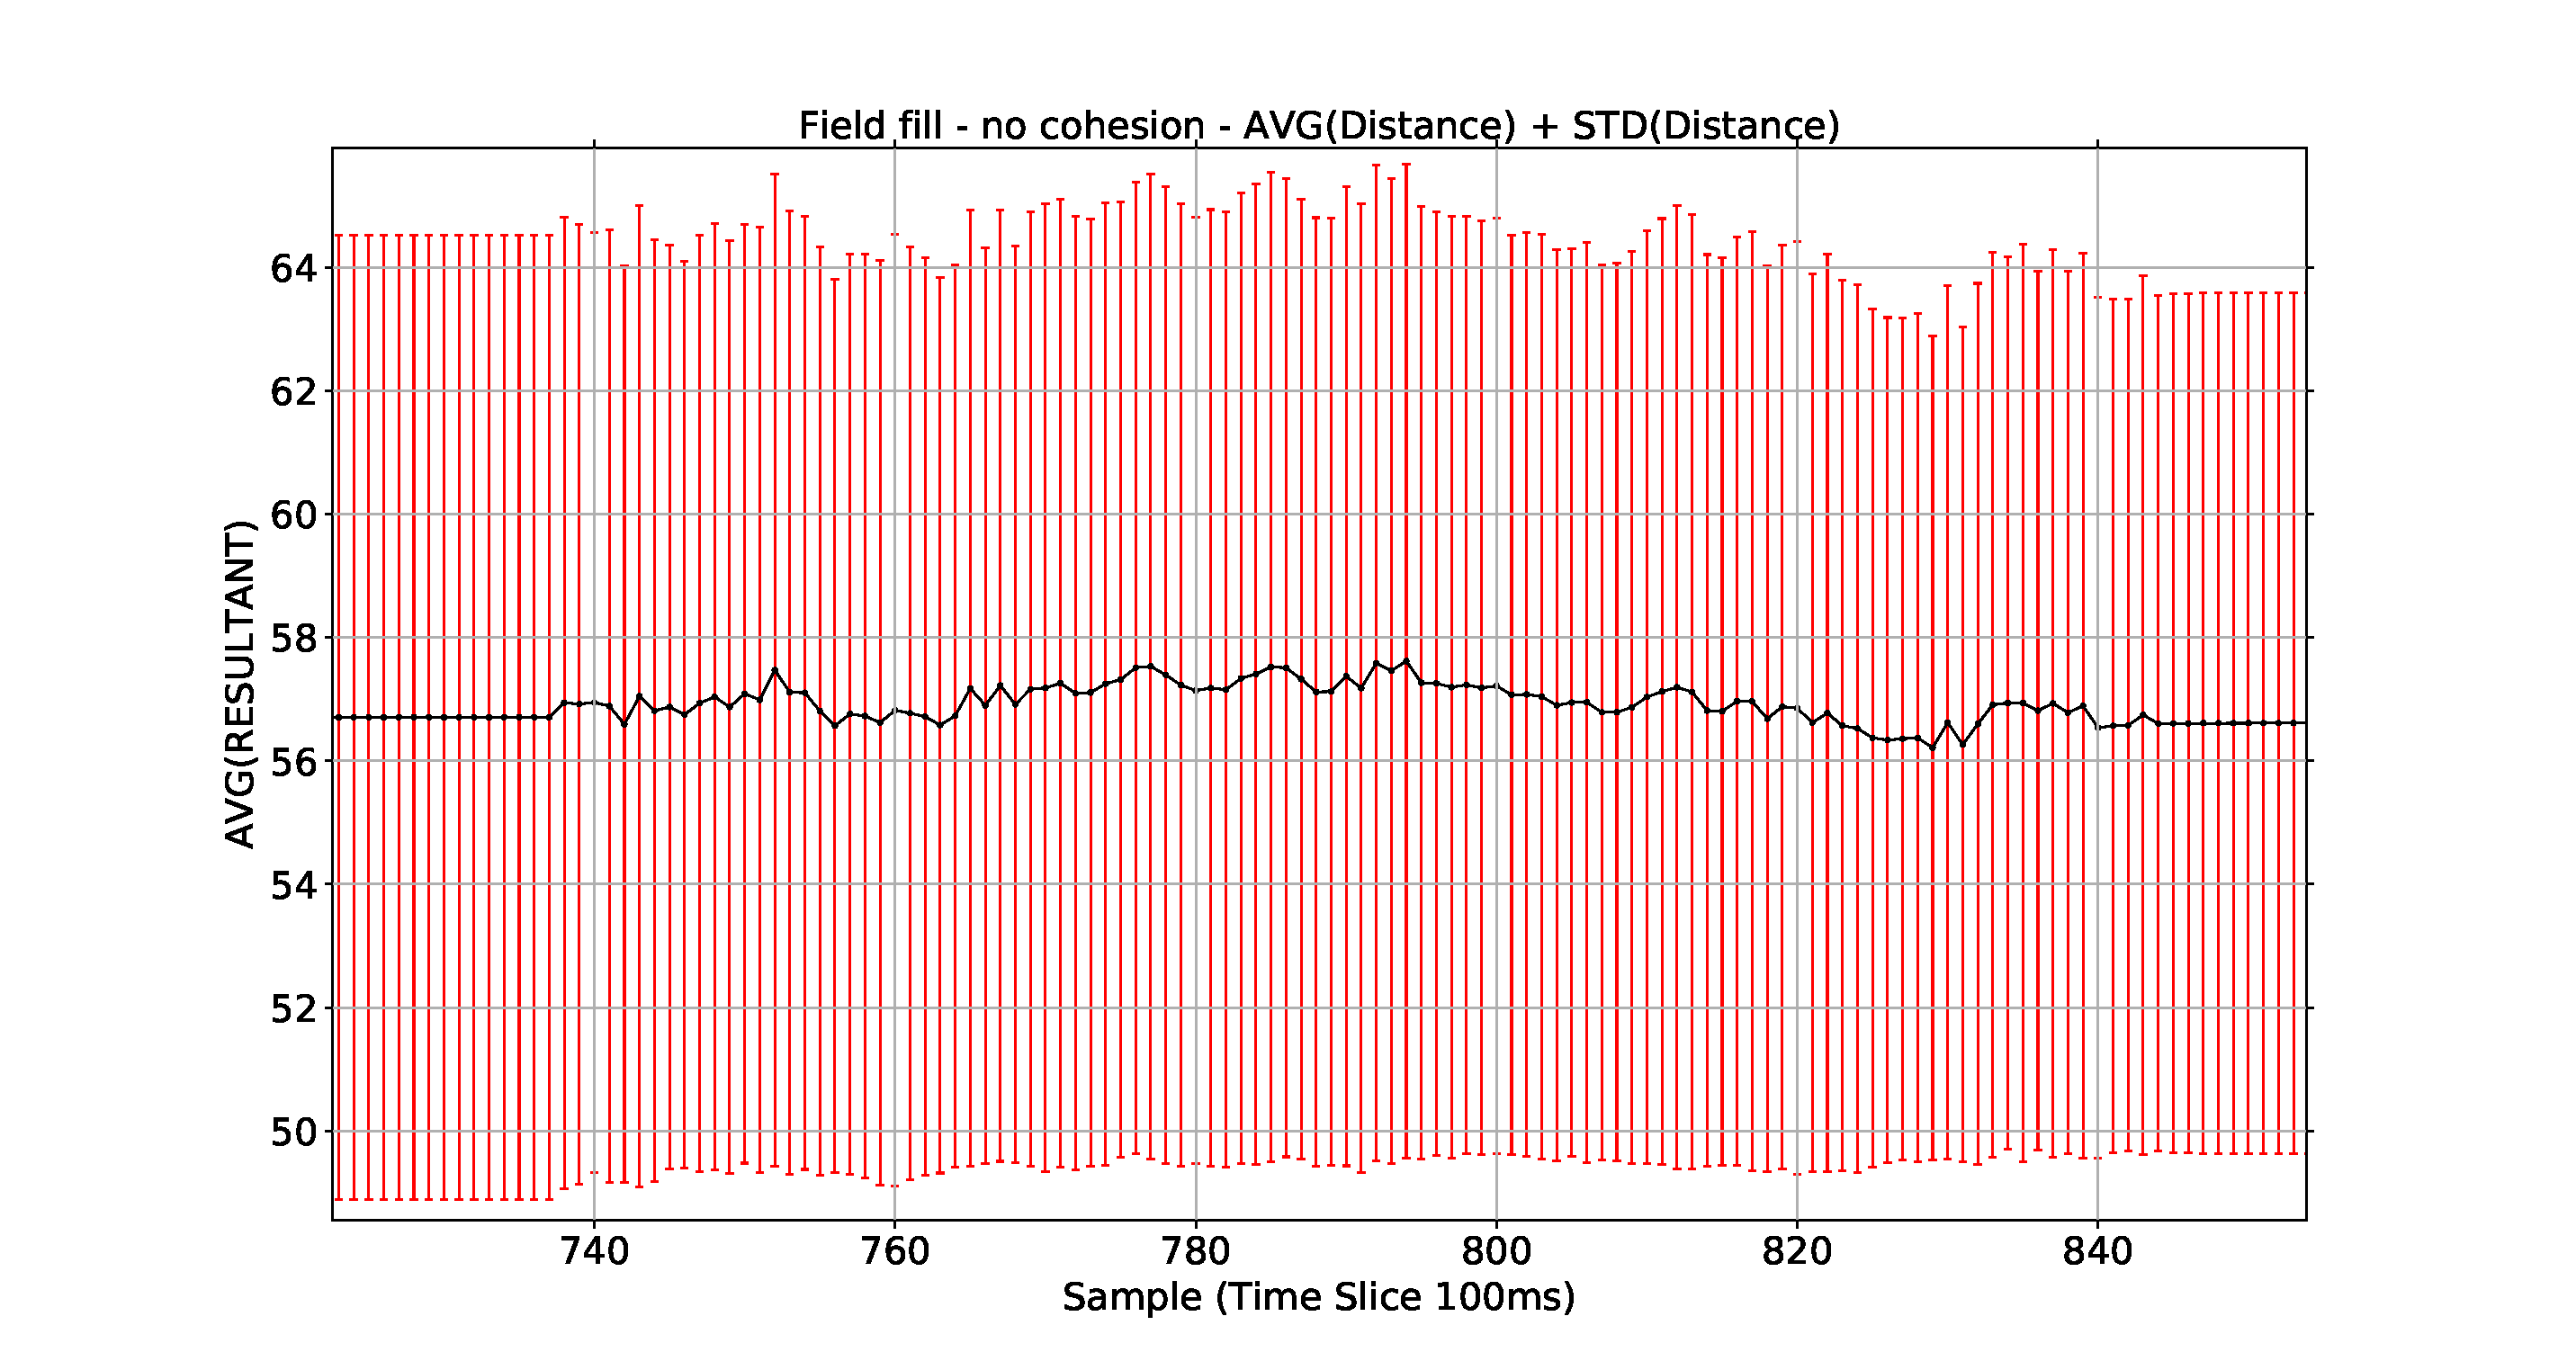
\includegraphics[width=8.5cm]{figures/REPELFILL5055-DIST-1-2}
\end{center}
\caption{Distance metric 70-85 seconds\label{emerge:REPELFILL5055-DIST-1-2}}
\end{figure}

Figure~\ref{emerge:REPELFILL5055-DIST-2-3} shows that at each increment the inter-agent average distances varies but the variance decreases as the swarm stabilises and the distribution improves. This improvement in distribution is the agents `spreading' more evenly as the swarm expands within the area. However after the last field effect increase at 230 seconds the swarm is no longer able to stabilise to a static state. 

\begin{figure}
\begin{center}
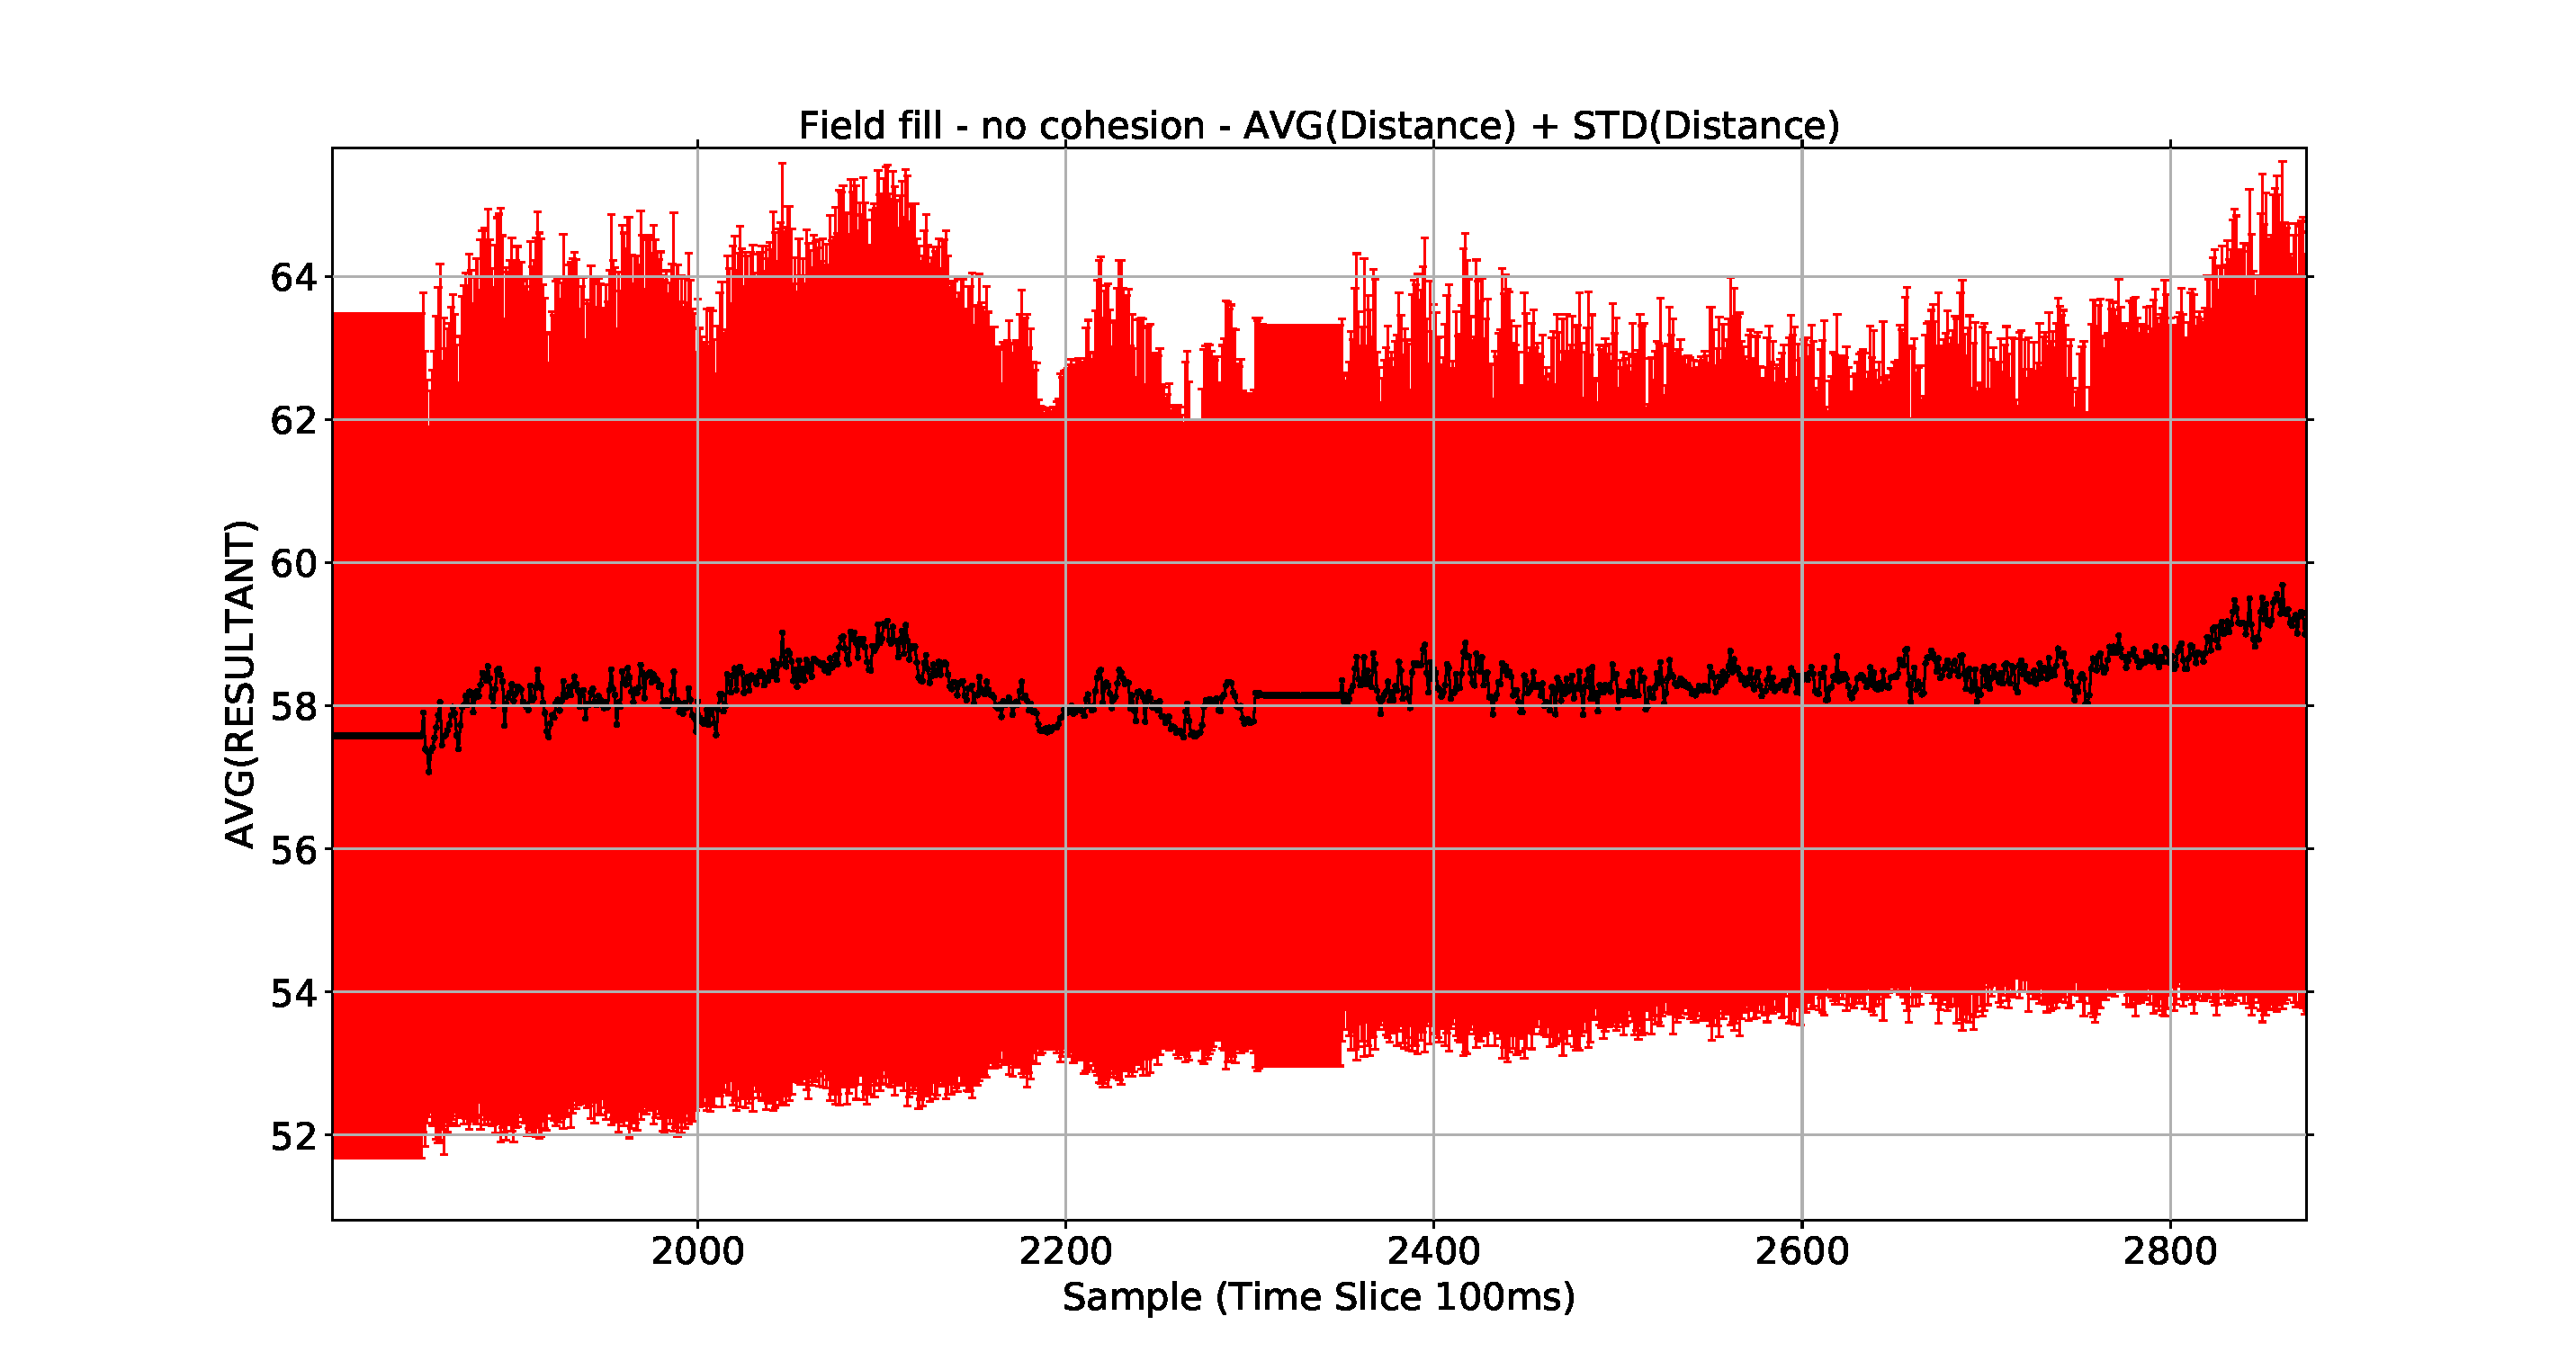
\includegraphics[width=8.5cm]{figures/REPELFILL5055-DIST-2-3}
\end{center}
\caption{Distance metric 180-280 seconds\label{emerge:REPELFILL5055-DIST-2-3}}
\end{figure}

Figure~\ref{emerge:REPELFILL5055-DIST-8} shows the effect of the final increment. The swarm expands but is unable to stabilise the system. The average distances fluctuate as the agents move to balance the \textit{inter-agent vectors} but the distances are unable to increase any further. The inter-agent distances are effected by the positioning of some of the agents preventing a regular shape to be formed this causes the distance variance to increase and the swarms structure starts to oscillate. These characteristics indicate that the area may be fully filled. The magnitude at this point is below zero~Figure~\ref{emerge:REPELFILL5055-MAG-8} which indicates expansion of the swarm is posible but not occuring. The conclusion therefore is that the swarm is fully expanded. The magnitude indicates a tendency for the swarm to expand but the distances are not increasing in line with the magnitude increase. 

\begin{figure}
\begin{center}
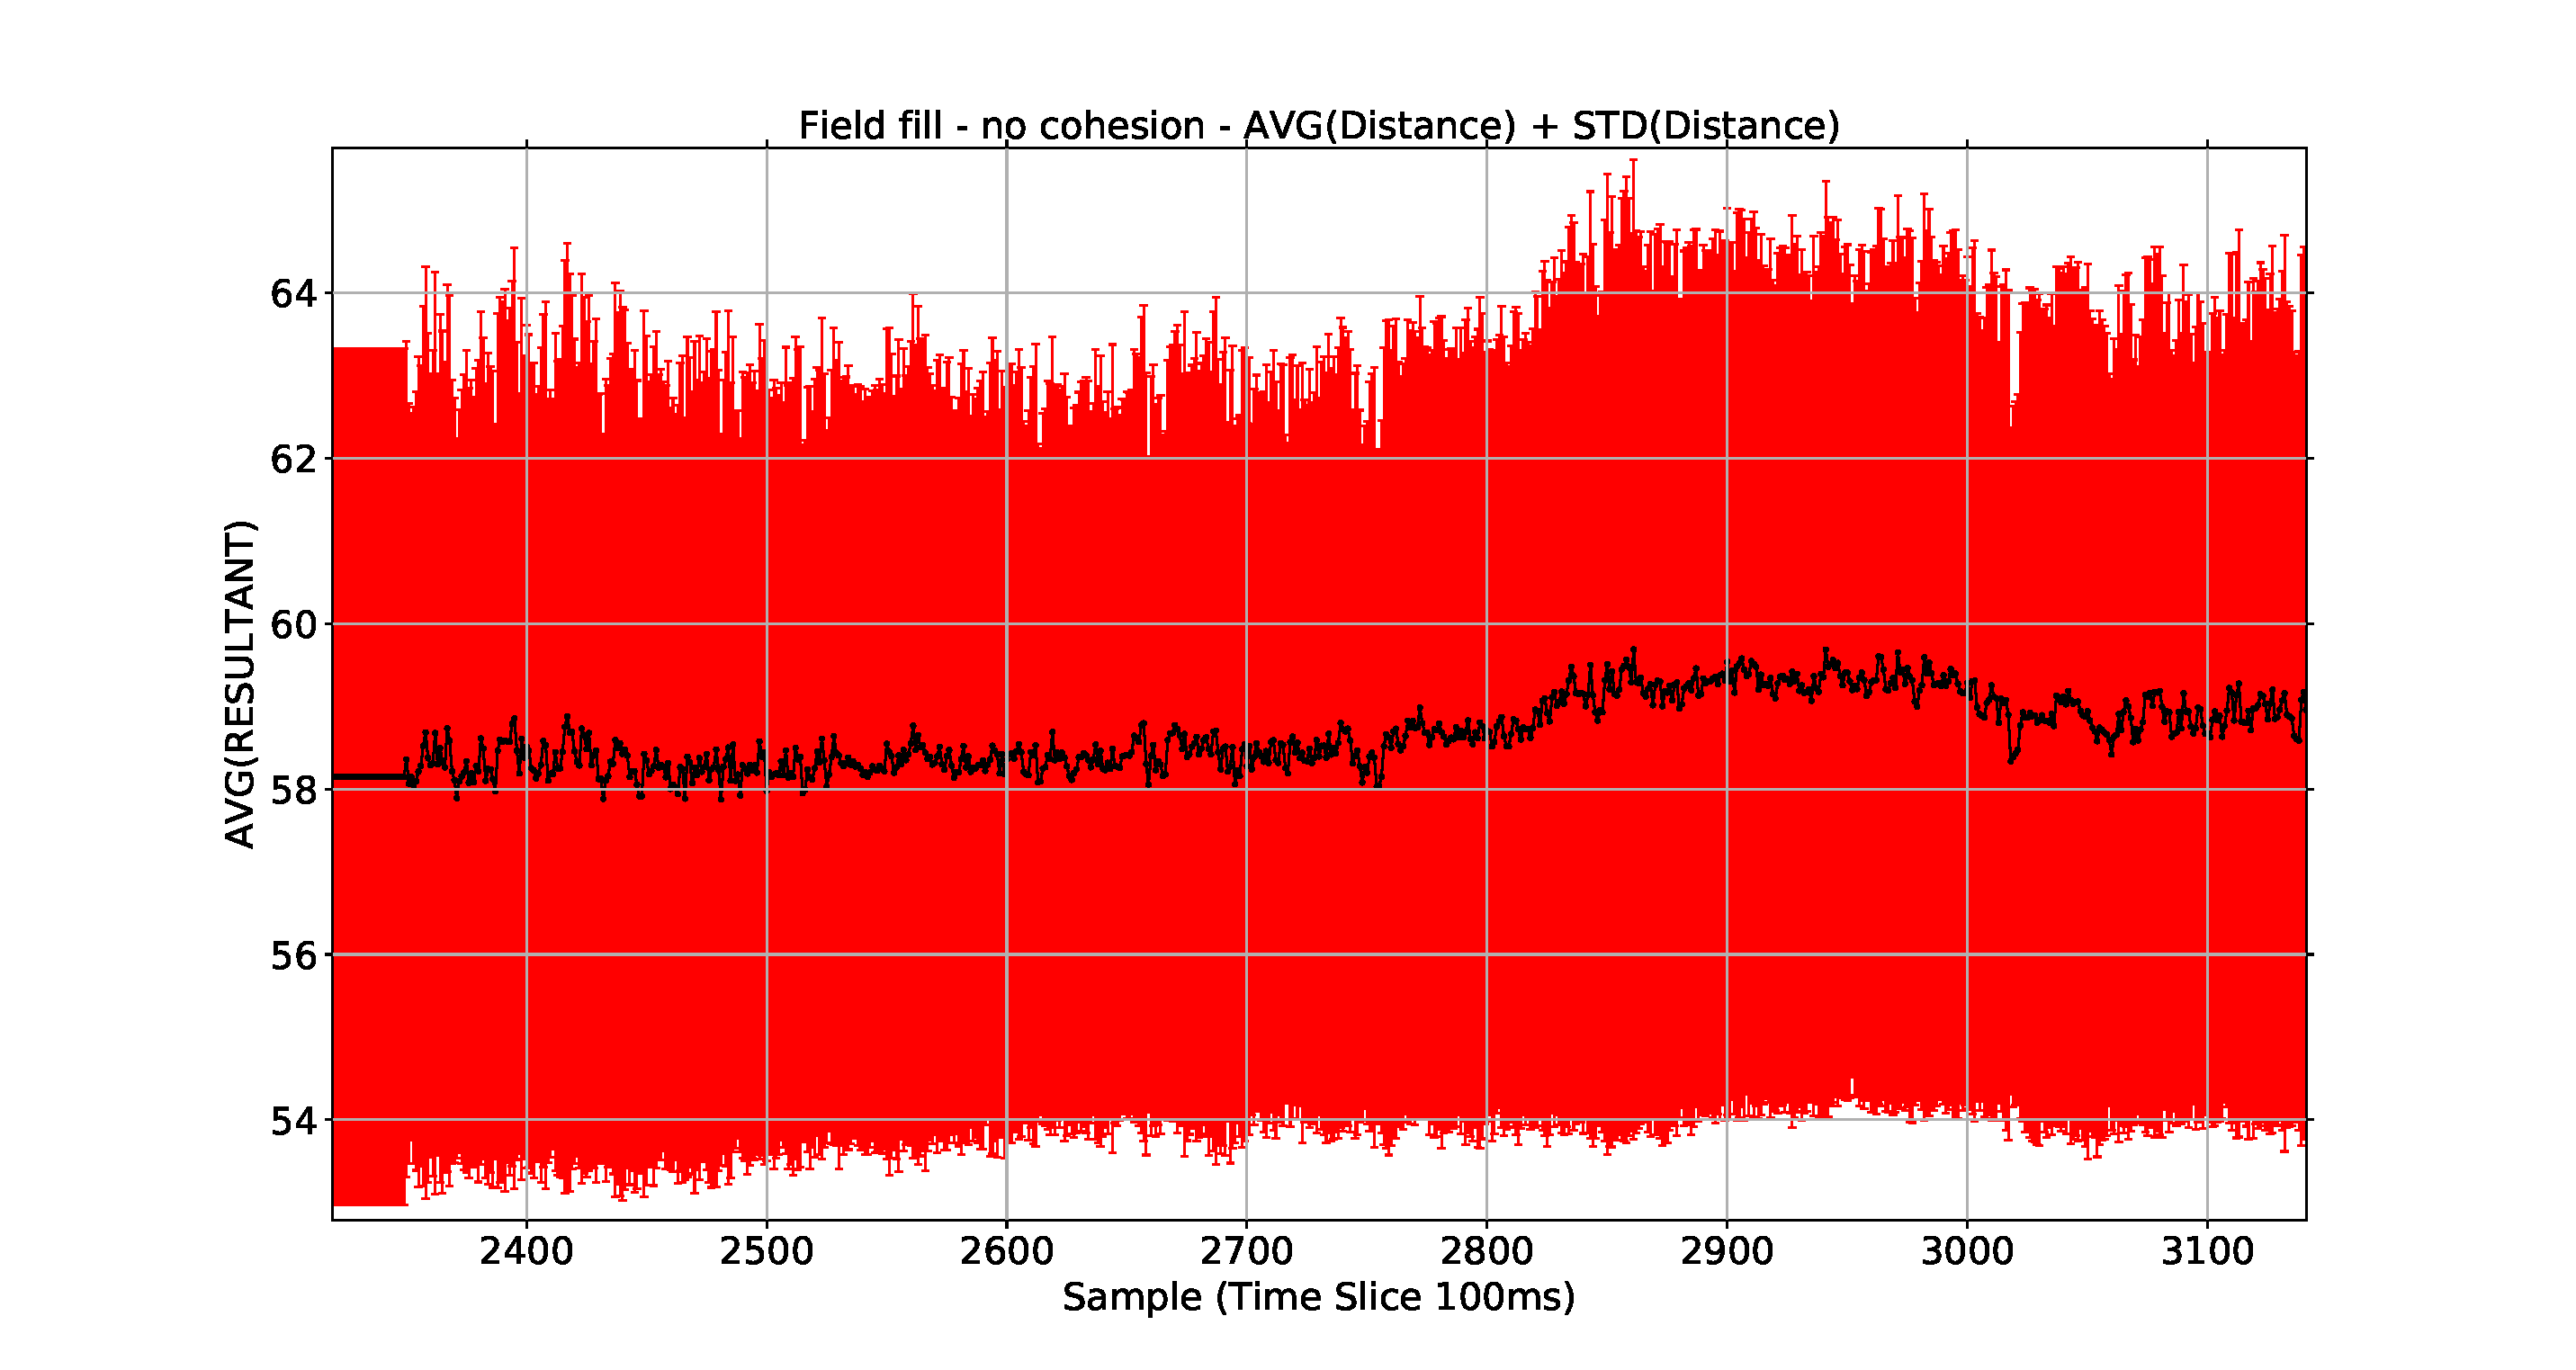
\includegraphics[width=8.5cm]{figures/REPELFILL5055-DIST-8}
\end{center}
\caption{Distance metric 235-315 seconds\label{emerge:REPELFILL5055-DIST-8}}
\end{figure}

\section{Conclusion}
Both of the flood fill techniques work successfully in filling the space. The use of the distance metric is limited in showing the full state state of a swarm due there being no indication of a static state. The \textit{inter-agent vector} metric provides an indication of the ability of the swarm to expand. Using the two metrics together allows the level of the flood filling of a space to be identified. A large distribution in distances indicates possible spaces in the distribution of the agents and ensuring the average \textit{inter-agent vector magnitude} becomes negative ensures the swarm will resolve anomalies in the distribution.

The difference in the approaches of using cohesion combined with repulsion and repulsion only provide two very different characteristics for determining the exit condition for the flood fill. The combination of repulsion and cohesion fields together result in a swarm that moves not only to fill the space but also to accommodate inter-agent relationships as a result the swarm is unable to obtain a static state. Using repulsion only provides clear indications when the space is not filling a space and allows `gaps' to occur in the swarms structure as the cohesion is not present even when agents are within visible `range'.

\bibliographystyle{plain}
\bibliography{thesis}

\end{document}
